% !TEX program = xelatex
% main.tex — 物理学家用数学方法 (Babusci et al.) 中文版
% XeLaTeX 工程主文件

\documentclass[11pt,a4paper]{book}

% ===== 中文支持 =====
\usepackage{ctex}

% ===== 英文字体 =====
\usepackage{fontspec}
\setmainfont{Times New Roman}
\setsansfont{Arial}

% ===== 数学 =====
\usepackage{amsmath,amssymb,amsfonts,amsthm}
\usepackage{bm}
\usepackage{mathtools}
\usepackage{slashed}

% ===== 图形 =====
\usepackage{graphicx}
\usepackage{float}
\usepackage{subcaption}
\usepackage[export]{adjustbox}

% ===== 列表 =====
\usepackage[shortlabels]{enumitem}

% ===== 表格 =====
\usepackage{array,booktabs}

% ===== 超链接与书签 =====
\usepackage[colorlinks=true,linkcolor=blue,citecolor=blue,urlcolor=blue]{hyperref}

% ===== 页面布局 =====
\usepackage[left=25mm,right=25mm,top=25mm,bottom=25mm]{geometry}

% ===== 目录深度 =====
\setcounter{tocdepth}{2}
\setcounter{secnumdepth}{3}

% ===== 图形搜索路径（按章节分目录） =====
\graphicspath{{figures/}}

% ===== 自定义宏 =====
\newcommand{\mat}[1]{\begin{pmatrix}#1\end{pmatrix}}
\newcommand{\vect}[1]{\bm{#1}}
\newcommand{\pauli}{\hat{\sigma}}
\newcommand{\spp}{\pauli_{+}}
\newcommand{\smm}{\pauli_{-}}
\newcommand{\sigx}{\pauli_{x}}
\newcommand{\sigy}{\pauli_{y}}
\newcommand{\sigz}{\pauli_{z}}
\newcommand{\tr}{\operatorname{Tr}}
\newcommand{\sincf}{\operatorname{sinc}}
\newcommand{\diag}[1]{\operatorname{diag}(#1)}
\newcommand{\sinc}{\operatorname{sinc}}
\newcommand{\erfi}{\operatorname{erfi}}
\newcommand{\erfc}{\operatorname{erfc}}
\newcommand{\sn}{\operatorname{sn}}
\newcommand{\cn}{\operatorname{cn}}
\newcommand{\dn}{\operatorname{dn}}
\newcommand{\sech}{\operatorname{sech}}

% ===== 定理类环境 =====
\newtheorem{theorem}{定理}[chapter]
\newtheorem{proposition}{命题}[chapter]
\newtheorem{exercise}{练习}[chapter]

% ===== 标题信息 =====
\title{物理学家用数学方法}
\author{Danilo Babusci \\ Giuseppe Dattoli \\ Silvia Licciardi \\ Elio Sabia}
\date{LaTeX 中文转写版}

\begin{document}

\frontmatter
\maketitle
\tableofcontents

\mainmatter

% ch1.tex — 第 1 章：矩阵、指数算子及其物理应用（中文版）
% 对应原书第 1–62 页（Sec. 1.1 – 1.6.7 + 参考文献）

\chapter{矩阵、指数算子及其物理应用}
\label{ch:1}

% ============================================================
\section{引言}
\label{sec:1.1}

矩阵及其相关形式体系是物理学与数学中广泛使用的工具。它们构成了处理经典与量子物理学中许多问题的支柱。因此，我们以对这些相关性质的简要回顾来开始本课程，目的是确定记号约定，并说明我们后续在求解具有物理意义的数学问题时所采用的技术细节。

我们的出发点是方程
\begin{equation}
\hat{A}\,\underline{\zeta} = \underline{b},
\label{eq:1.1.1}
\end{equation}
其中
\[
\hat{A} = \mat{\alpha_{11} & \alpha_{12} \\ \alpha_{21} & \alpha_{22}},\qquad
\underline{\zeta} = \mat{z_{1} \\ z_{2}},\qquad
\underline{b} = \mat{b_{1} \\ b_{2}},\qquad
\forall\,\alpha_{ij},z_{i},b_{i}\in\mathbb{C}.
\]
方程~\eqref{eq:1.1.1} 可以看作一次代数方程的推广。只要我们把矩阵视为普通数的推广，其解就可以写成
\begin{equation}
\underline{\zeta} = \hat{A}^{-1}\,\underline{b},
\label{eq:1.1.3}
\end{equation}
这与一次代数方程的解的形式相仿。这样的形式解只有在矩阵 $\hat{A}$ 非奇异、即可逆时才有意义。我们曾隐式地假定
\begin{equation}
\hat{A}\,\hat{A}^{-1} = \hat{1},
\label{eq:1.1.4}
\end{equation}
其中实单位矩阵为
\[
\hat{1} = \mat{1 & 0 \\ 0 & 1},
\]
它满足
\[
\hat{1}\,\hat{B} = \hat{B}\,\hat{1} = \hat{B},\qquad \hat{1}\,\underline{\zeta} = \underline{\zeta}.
\]

对于二维情形，$\hat{A}$ 的逆为
\[
\hat{A}^{-1} = \frac{1}{\Delta}\mat{\alpha_{22} & -\alpha_{12} \\ -\alpha_{21} & \alpha_{11}},\qquad
\Delta = \alpha_{11}\alpha_{22} - \alpha_{12}\alpha_{21}.
\]
若行列式为零，则矩阵是奇异（不可逆）的。

与单位矩阵一道，我们还引入\emph{虚矩阵}
\begin{equation}
\hat{i} = \mat{0 & 1 \\ -1 & 0},\qquad \hat{i}^{2} = -\hat{1}.
\label{eq:1.1.9}
\end{equation}

矩阵的函数通过其 Maclaurin 展开定义
\[
f(\hat{A}) = \sum_{n=0}^{\infty}\frac{f^{(n)}(0)}{n!}\,\hat{A}^{n}.
\]
对 $\hat{i}$ 取指数便得到矩阵形式的 Euler 公式：
\begin{align}
e^{\alpha\hat{i}}
&= \sum_{n=0}^{\infty}\frac{\alpha^{n}}{n!}\,\hat{i}^{n}
 = \cos\alpha\,\hat{1} + \sin\alpha\,\hat{i} \notag \\
&= \mat{\cos\alpha & \sin\alpha \\ -\sin\alpha & \cos\alpha}
 = \hat{R}(\alpha).
\label{eq:1.1.17}
\end{align}
因此，虚矩阵的指数化给出二维旋转矩阵。

\emph{双曲单位矩阵}
\[
\hat{h} = \mat{0 & 1 \\ 1 & 0},\qquad \hat{h}^{2} = \hat{1},
\]
给出
\[
e^{\alpha\hat{h}} = \mat{\cosh\alpha & \sinh\alpha \\ \sinh\alpha & \cosh\alpha}
= \hat{R}_{h}(\alpha).
\]

这三个单位不互相对易：
\[
[\hat{i},\hat{h}] = 2\hat{t},\qquad
\hat{t} = \mat{1 & 0 \\ 0 & -1}.
\]
任何 $2\times 2$ 矩阵都可以展开为
\[
\mat{\alpha_{11} & \alpha_{12} \\ \alpha_{21} & \alpha_{22}}
= a\,\hat{1} + b\,\hat{i} + c\,\hat{h} + d\,\hat{t}.
\]

厄米共轭定义为
\[
\hat{A}^{\dagger} = \mat{\alpha_{11}^{*} & \alpha_{21}^{*} \\ \alpha_{12}^{*} & \alpha_{22}^{*}}.
\]
我们有 $\hat{i}^{\dagger} = -\hat{i}$（反厄米），而 $\hat{h},\hat{t},\hat{1}$ 是厄米的。

% ============================================================
\section{Pauli 矩阵}
\label{sec:1.2}

定义升降算子
\[
\spp = \mat{0 & 1 \\ 0 & 0},\qquad
\smm = \mat{0 & 0 \\ 1 & 0},\qquad
\spp^{2} = \smm^{2} = \hat{0},
\]
于是
\[
\hat{i} = \spp - \smm.
\]
Pauli--$z$ 矩阵为
\[
\sigz = \frac{1}{2}\hat{t} = \mat{\tfrac{1}{2} & 0 \\ 0 & -\tfrac{1}{2}}.
\]

对易关系为
\begin{equation}
[\spp,\smm] = 2\sigz,\qquad
[\sigz,\spp] = \spp,\qquad
[\sigz,\smm] = -\smm,
\label{eq:1.2.8}
\end{equation}
它们正是 $SU(2)$ 代数。标准 Pauli 矢量是
\[
\sigx = \frac{1}{2}(\spp+\smm),\quad
\sigy = \frac{1}{2i}(\spp-\smm),\quad
\sigz = \frac{1}{2}\mat{1 & 0 \\ 0 & -1},
\]
且
\[
[\pauli_{j},\pauli_{k}] = i\,\varepsilon_{jkl}\,\pauli_{l}.
\]

对于哈密顿量 $\hat{H} = \hbar\,\vec{\Omega}\!\cdot\!\vec{\sigma}$，演化算子为
\[
\hat{U}(t) = e^{-i\Omega t\,\vec{n}\!\cdot\!\vec{\sigma}}
= \cos\!\left(\frac{\Omega t}{2}\right)\hat{1}
- 2i\sin\!\left(\frac{\Omega t}{2}\right)\vec{n}\!\cdot\!\vec{\sigma}.
\]

对于无迹反厄米 $2\times 2$ 矩阵，一个有用的解缠（disentanglement）公式为
\[
e^{\alpha(\spp-\smm)}
= e^{2h(\alpha)\sigz}\,e^{f(\alpha)\spp}\,e^{-g(\alpha)\smm},
\]
其中 $h(0)=f(0)=g(0)=0$，且（对这一特殊情形）
\[
e^{h(\alpha)} = \sec\alpha,\qquad
f(\alpha) = \tfrac{1}{2}\sin 2\alpha,\qquad
g(\alpha) = \tan\alpha.
\]

对于一般的 $\tr\hat{\alpha}\neq 0$ 的 $2\times 2$ 矩阵 $\hat{\alpha}$，
\[
e^{\hat{\alpha}} = \mat{A_{11} & A_{12} \\ A_{21} & A_{22}},
\]
其中（$\Delta = (\alpha_{11}-\alpha_{22})^{2}+4\alpha_{12}\alpha_{21}$）
\begin{align*}
A_{11} &= \left\{\frac{\alpha_{11}-\alpha_{22}}{\sqrt{\Delta}}\sinh\frac{\sqrt{\Delta}}{2}
           + \cosh\frac{\sqrt{\Delta}}{2}\right\}e^{\frac{1}{2}\tr\hat{\alpha}},\\
A_{22} &= \left\{-\frac{\alpha_{11}-\alpha_{22}}{\sqrt{\Delta}}\sinh\frac{\sqrt{\Delta}}{2}
           + \cosh\frac{\sqrt{\Delta}}{2}\right\}e^{\frac{1}{2}\tr\hat{\alpha}},\\
\frac{A_{12}}{\alpha_{12}} &= \frac{A_{21}}{\alpha_{21}}
 = \frac{2}{\sqrt{\Delta}}\sinh\frac{\sqrt{\Delta}}{2}\,e^{\frac{1}{2}\tr\hat{\alpha}}.
\end{align*}

% ============================================================
\section{\texorpdfstring{$2\times 2$}{2x2} 矩阵的应用}
\label{sec:1.3}

\subsection{经典光学：光线传播与 ABCD 定律}

近轴光线用 $\mat{r & \vartheta}^{T}$ 描述。长度为 $d$ 的自由空间：
\[
\hat{O} = \mat{1 & d \\ 0 & 1} = e^{d\spp}.
\]
焦距为 $f$ 的薄透镜：
\[
\hat{F} = \mat{1 & 0 \\ -1/f & 1} = e^{-\frac{1}{f}\smm},\qquad
\hat{D} = \mat{1 & 0 \\ 1/f & 1} = e^{\frac{1}{f}\smm}.
\]
扩束器（squeeze）：
\[
e^{b\sigz} = \mat{e^{b} & 0 \\ 0 & e^{-b}}.
\]
ABCD 定律是
\[
\mat{r \\ \vartheta}_{\mathrm{out}}
= \mat{A & B \\ C & D}
  \mat{r \\ \vartheta}_{\mathrm{in}}.
\]

\subsection{量子力学}

磁场 $\vec{B}=B\hat{y}$ 中自旋 $\tfrac{1}{2}$ 粒子的 Pauli 方程：
\[
i\hbar\,\partial_{t}\underline{\Phi}
= -\frac{q\hbar}{2m}\,\vec{\sigma}\!\cdot\!\vec{B}\,\underline{\Phi}
\;\Longrightarrow\;
\partial_{t}\underline{\Phi}
= \omega_{c}(\spp-\smm)\underline{\Phi},\qquad
\omega_{c} = \frac{qB}{4m}.
\]
解：$\underline{\Phi}(t) = \hat{R}(\omega_{c}t)\,\underline{\Phi}_{0}$。

二能级系统：
\[
i\hbar\,\partial_{t}\mat{a_{+} \\ a_{-}}
= \bigl(\omega\sigz + 2\Omega\sigy\bigr)\mat{a_{+} \\ a_{-}},
\]
其中演化矩阵即上文给出的 $SU(2)$ 旋转矩阵。

\subsection{粒子物理：Kaon 混合}

中性 Kaon 态：
\[
|K^{0}\rangle = |\bar{s}d\rangle,\qquad
|\bar{K}^{0}\rangle = |\bar{d}s\rangle.
\]
CP 本征态：
\[
|K_{S}\rangle = \frac{1}{\sqrt{2}}\bigl(|K^{0}\rangle + |\bar{K}^{0}\rangle\bigr),\qquad
|K_{L}\rangle = \frac{1}{\sqrt{2}}\bigl(|K^{0}\rangle - |\bar{K}^{0}\rangle\bigr).
\]
用非厄米哈密顿量
\[
\hat{H} = \mat{E_{S}-i\Gamma_{S}/2 & 0 \\ 0 & E_{L}-i\Gamma_{L}/2}
\]
进行演化，得到振荡的跃迁几率
\[
\bigl|\langle\bar{K}^{0}\mid\Psi_{K}(t)\rangle\bigr|^{2}
= \frac{1}{4}\Bigl(e^{-t/\tau_{S}} + e^{-t/\tau_{L}}
- 2e^{-t/\tau^{*}}\cos\bigl((\omega_{S}-\omega_{L})t\bigr)\Bigr).
\]

% ============================================================
\section{Cabibbo 角与跷跷板机制}
\label{sec:1.4}

$s$--$d$ 扇区中的味混合：
\[
\mat{d' \\ s'} = e^{\vartheta\hat{i}}\mat{d \\ s}
= \mat{\cos\vartheta & \sin\vartheta \\ -\sin\vartheta & \cos\vartheta}\mat{d \\ s}.
\]
跷跷板中微子质量矩阵：
\[
\hat{m}_{\nu} = \mat{0 & m_{D} \\ m_{D} & M_{NHL}},\qquad M_{NHL}\gg m_{D}.
\]

% ============================================================
\section{Gell-Mann 矩阵与 Pauli 矩阵}
\label{sec:1.5}

\subsection{自旋合成}

\[
\tfrac{1}{2}\otimes\tfrac{1}{2} = 0\oplus 1,\qquad
\tfrac{1}{2}\otimes\tfrac{1}{2}\otimes\tfrac{1}{2}
= \tfrac{1}{2}\oplus\tfrac{1}{2}\oplus\tfrac{3}{2}.
\]

\subsection{Gell-Mann 矩阵}

八个 $3\times 3$ 的 Gell-Mann 矩阵 $\hat{\lambda}_{\alpha}$（$\alpha=1,\dots,8$）满足
\[
[\hat{\lambda}_{\alpha},\hat{\lambda}_{\beta}] = i\,f_{\alpha\beta\gamma}\,\hat{\lambda}_{\gamma},\qquad
\tr(\hat{\lambda}_{\alpha}\hat{\lambda}_{\beta}) = 2\delta_{\alpha\beta}.
\]
具体地，
\begin{align*}
\hat{\lambda}_{1}&=\mat{0&1&0\\1&0&0\\0&0&0},&
\hat{\lambda}_{2}&=\mat{0&-i&0\\i&0&0\\0&0&0},&
\hat{\lambda}_{3}&=\mat{1&0&0\\0&-1&0\\0&0&0},\\
\hat{\lambda}_{4}&=\mat{0&0&1\\0&0&0\\1&0&0},&
\hat{\lambda}_{5}&=\mat{0&0&-i\\0&0&0\\i&0&0},&
\hat{\lambda}_{6}&=\mat{0&0&0\\0&0&1\\0&1&0},\\
\hat{\lambda}_{7}&=\mat{0&0&0\\0&0&-i\\0&i&0},&
\hat{\lambda}_{8}&=\frac{1}{\sqrt{3}}\mat{1&0&0\\0&1&0\\0&0&-2}.
\end{align*}

\subsection{味与自旋}

介子：$3\otimes\bar{3} = 1\oplus 8$。\\
重子：$3\otimes 3\otimes 3 = 1\oplus 8\oplus 8\oplus 10$。

质子波函数（味 $\times$ 自旋）：
\[
|p\rangle = \frac{1}{2\sqrt{3}}\,
(duu\;\;udu\;\;uud)\,
\mat{2&-1&-1\\-1&2&-1\\-1&-1&2}\,
\mat{\downarrow\uparrow\uparrow \\ \uparrow\downarrow\uparrow \\ \uparrow\uparrow\downarrow}.
\]

\subsection{色与 QCD}

色三重态 $R,G,B$ 使重子在色指标下为反对称：
\[
|\Omega^{-}\rangle = \frac{1}{\sqrt{6}}\sum_{ijk}\varepsilon_{ijk}\,|s_{i}s_{j}s_{k}\rangle.
\]
胶子属于 $SU(3)$ 色八重态。

% ============================================================
\section{结语}
\label{sec:1.6}

\subsection{矢量微分方程与矩阵}
\label{sec:1.6.1}

Pauli 矢量的类 Heisenberg 方程：
\[
\frac{d}{dt}\vec{\sigma} = \vec{\Omega}\times\vec{\sigma}.
\]
解（Rodrigues 旋转）：
\begin{align}
\vec{\sigma}(t)
&= \cos(\Omega t)\,\vec{\sigma}_{0}
 + \sin(\Omega t)\,(\vec{n}\times\vec{\sigma}_{0}) \notag \\
&\quad + \bigl[1-\cos(\Omega t)\bigr]\,(\vec{n}\!\cdot\!\vec{\sigma}_{0})\,\vec{n}.
\label{eq:rodrigues}
\end{align}
非齐次情形：
\[
\frac{d}{dt}\vec{\sigma} = \vec{\Omega}\times\vec{\sigma} + \vec{\gamma}
\;\Longrightarrow\;
\vec{\sigma}(t) = e^{t[\vec{\Omega}]}\vec{\sigma}_{0}
+ \int_{0}^{t} e^{(t-t')[\vec{\Omega}]}\,\vec{\gamma}\,dt'.
\]

\subsection{矩阵、矢量方程与旋转}
\label{sec:1.6.2}

对于 $\vec{S} = (S_{1},S_{2},S_{3})^{T}$，
\[
\frac{d}{dt}\mat{S_{1}\\S_{2}\\S_{3}}
= \mat{0&-\Omega_{3}&\Omega_{2}\\
        \Omega_{3}&0&-\Omega_{1}\\
       -\Omega_{2}&\Omega_{1}&0}
  \mat{S_{1}\\S_{2}\\S_{3}}.
\]
演化算子 $\hat{U}(t)$ 即 Rodrigues 旋转矩阵
\[
\hat{U}(t) = \hat{1} + \frac{\sin\Omega t}{\Omega}\,\hat{\Omega}
+ \frac{1-\cos\Omega t}{\Omega^{2}}\,\hat{\Omega}^{2},
\]
其中 $\Omega = \sqrt{\Omega_{1}^{2}+\Omega_{2}^{2}+\Omega_{3}^{2}}$。

\subsection{Cabibbo--Kobayashi--Maskawa 矩阵}
\label{sec:1.6.3}

对三代夸克的推广：
\[
\mat{d'\\s'\\b'} = e^{\hat{\Omega}}\mat{d\\s\\b},
\]
其中 $\Omega_{3}=\vartheta_{c}$，$\Omega_{2}=x\vartheta_{c}^{2}$，$\Omega_{1}=y\vartheta_{c}^{3}$，且 $\vartheta_{c}\simeq 0.22$ rad。

\subsection{Frenet--Serret 方程}
\label{sec:1.6.4}

\[
\frac{d}{ds}\mat{T\\N\\B}
= \mat{0&\kappa&0\\-\kappa&0&\tau\\0&-\tau&0}
  \mat{T\\N\\B}.
\]

\subsection{矩阵、旋转与 Euler 角}
\label{sec:1.6.5}

Euler 角分解：
\begin{align*}
\hat{R}
&= e^{\alpha\hat{J}_{z}}\,e^{\beta\hat{J}_{y}}\,e^{\gamma\hat{J}_{z}} \\
&= \mat{\cos\alpha&-\sin\alpha&0\\\sin\alpha&\cos\alpha&0\\0&0&1}
   \mat{1&0&0\\0&\cos\beta&-\sin\beta\\0&\sin\beta&\cos\beta}
   \mat{\cos\gamma&-\sin\gamma&0\\\sin\gamma&\cos\gamma&0\\0&0&1}.
\end{align*}

\subsection{四矢量与 Lorentz 变换}
\label{sec:1.6.6}

Minkowski 度规：
\[
\eta_{\mu\nu} = \mat{-1&0&0&0\\0&1&0&0\\0&0&1&0\\0&0&0&1}.
\]
沿 $x$ 方向的 Lorentz boost：
\[
\mat{ct'\\x'\\y'\\z'}
= \mat{\gamma&-\gamma\beta&0&0\\-\gamma\beta&\gamma&0&0\\0&0&1&0\\0&0&0&1}
  \mat{ct\\x\\y\\z},
\qquad \gamma = \frac{1}{\sqrt{1-\beta^{2}}}.
\]

\subsection{Dirac 矩阵}
\label{sec:1.6.7}

分块形式（用 $2\times 2$ 块 $\hat{1},\hat{i},\hat{h},\hat{t}$）：
\[
\gamma^{0} = \mat{\hat{1}&\hat{0}\\\hat{0}&-\hat{1}},\quad
\gamma^{1} = \mat{\hat{0}&\hat{h}\\-\hat{h}&\hat{0}},\quad
\gamma^{2} = -i\mat{\hat{0}&\hat{i}\\-\hat{i}&\hat{0}},\quad
\gamma^{3} = \mat{\hat{0}&\hat{t}\\-\hat{t}&\hat{0}}.
\]
以及
\[
\gamma^{5} = i\gamma^{0}\gamma^{1}\gamma^{2}\gamma^{3}
= \mat{\hat{0}&\hat{1}\\\hat{1}&\hat{0}}.
\]

Dirac 方程：
\[
i\hbar\,\partial_{t}\Psi = \vec{\alpha}\!\cdot\!\vec{p}\,\Psi + \beta\,mc^{2}\Psi.
\]

Foldy--Wouthuysen 变换：
\[
\hat{U} = e^{\beta\vec{\alpha}\!\cdot\!\vec{p}\,\vartheta}
= \cos\theta + \beta\,\vec{\alpha}\!\cdot\!\vec{n}_{p}\sin\theta,\qquad
\vec{n}_{p} = \frac{\vec{p}}{p},
\]
其中 $\tan(2\vartheta) = p/(mc)$。

% ============================================================
\section*{第 1 章参考文献}
\addcontentsline{toc}{section}{第 1 章参考文献}

\begin{thebibliography}{99}

\bibitem{gantmaker} F.~R.\ Gantmaker, \emph{The Theory of Matrices}, Chelsea, New York, 1959.

\bibitem{lancaster} P.~Lancaster, M.~Tismenetsky, \emph{The Theory of Matrices with Applications}, Academic Press, 1985.

\bibitem{bronson1} R.~Bronson, \emph{Matrix Methods: An Introduction}, Academic Press, 1970.

\bibitem{bronson2} R.~Bronson, \emph{Schaum's Outline of Theory and Problems of Matrix Operations}, McGraw-Hill, 1989.

\bibitem{brown} W.~Brown, \emph{Matrices and Vector Spaces}, Marcel Dekker, 1991.

\bibitem{leonhardt} U.~Leonhardt, \emph{Essential Quantum Optics}, Cambridge University Press, 2000.

\bibitem{gasiorowicz} S.~Gasiorowicz, \emph{Quantum Physics}, Wiley, 1974.

\bibitem{goldstein} H.~Goldstein, \emph{Classical Mechanics}, 2nd ed., Addison-Wesley, 1980.

\bibitem{dattoli1990} G.~Dattoli, M.~Richetta, G.~Schettini, A.~Torre,
``Lie algebraic methods and solutions of linear partial differential equations'', \emph{J.\ Math.\ Phys.}\ \textbf{31}, 2856 (1990).

\bibitem{wei1963} J.~Wei, E.~Norman,
``Lie algebraic solution of linear differential equations'', \emph{J.\ Math.\ Phys.}\ \textbf{4}, 575 (1963).

\bibitem{vanderlugt} A.~Vander Lugt,
``Operational Notation for the Analysis and Synthesis of Optical Data Processing Systems'', \emph{Proc.\ IEEE} \textbf{54}, 1055 (1966).

\bibitem{stoler} D.~Stoler, ``Operator Methods in Physical Optics'', \emph{J.\ Opt.\ Soc.\ Am.}\ \textbf{71}, 334 (1981).

\bibitem{bacry} H.~Bacry, M.~Cadilhac, ``Metaplectic Group and Fourier Optics'', \emph{Phys.\ Rev.\ A} \textbf{23}, 2533 (1981).

\bibitem{sanchez} J.~Sanchez-Mandragon, K.~B.~Wolf, \emph{Lie Methods in Optics}, Springer, 1986.

\bibitem{dattoli1988} G.~Dattoli, A.~Torre, J.~C.~Gallardo,
``Operatorial methods in Optics'', \emph{Riv.\ Nuovo Cimento} \textbf{11}, 1 (1988).

\bibitem{torre2005} A.~Torre, \emph{Linear Ray and Wave Optics in Phase Space}, Elsevier, 2005.

\bibitem{feynman1957} R.~P.~Feynman, L.~P.~Vernon, R.~W.~Hellwarth,
``Geometrical Representation of the Schrodinger Equation to Solve Maser Problems'', \emph{J.\ Appl.\ Phys.}\ \textbf{28}, 49 (1957).

\bibitem{wu1957} C.~S.~Wu \emph{et al.}, ``Experimental Test of Parity Conservation in Beta Decay'', \emph{Phys.\ Rev.}\ \textbf{105}, 1413 (1957).

\bibitem{yariv} A.~Yariv, \emph{Quantum Electronics}, Wiley, 1985.

\bibitem{hallen} L.~Hallen, J.~H.~Eberly, \emph{Optical Resonance and Two-Level Atoms}, Wiley, 1975.

\bibitem{baym} G.~Baym, \emph{Lectures on Quantum Mechanics}, Benjamin, 1969.

\bibitem{cabibbo} N.~Cabibbo, ``Unitary Symmetry and Leptonic Decays'', \emph{Phys.\ Rev.\ Lett.}\ \textbf{10}, 531 (1963).

\bibitem{kobayashi} M.~Kobayashi, T.~Maskawa,
``CP Violation in the Renormalizable Theory of Weak Interaction'', \emph{Prog.\ Theor.\ Phys.}\ \textbf{49}, 652 (1973).

\bibitem{wolfenstein} L.~Wolfenstein, ``Parametrization of the Kobayashi-Maskawa Matrix'', \emph{Phys.\ Rev.\ Lett.}\ \textbf{51}, 1945 (1983).

\bibitem{dattoli1994} G.~Dattoli, ``Weak mixing angles, CP-violating phase and exponential parametrization of the Cabibbo-Kobayashi-Maskawa matrix'', \emph{Nuovo Cim.\ A} \textbf{107}, 1243 (1994).

\bibitem{mohapatra} R.~N.~Mohapatra, ``Physics of Neutrino Masses'', SLAC Summer Institute (SSI04), 2004.

\bibitem{gellmann} M.~Gell-Mann, \emph{The Eightfold Way}, Benjamin, 1964.

\bibitem{lichtenberg} D.~B.~Lichtenberg, \emph{Unitary Symmetry and Elementary Particles}, Academic Press, 1978.

\bibitem{peskin} M.~E.~Peskin, D.~V.~Schroeder, \emph{An Introduction to Quantum Field Theory}, Addison Wesley, 1995.

\bibitem{mangano} M.~L.~Mangano, ``Introduction to QCD'', in \emph{Proc.\ 1998 European School of High-Energy Physics}.

\bibitem{babusci2011} D.~Babusci, G.~Dattoli, E.~Sabia,
``Operational Methods and Lorentz Type Equations'', \emph{J.\ Phys.\ Math.}\ \textbf{3}, P110601 (2011).

\bibitem{varshalovich} D.~A.~Varshalovich, A.~N.~Moskalev, V.~K.~Khersonskii,
\emph{Quantum Theory of Angular Momentum}, World Scientific, 1988.

\bibitem{morin} D.~Morin, \emph{Relativity (Kinematics)}, Ch.~11, Harvard University, 2007.

\bibitem{good} R.~H.~Good Jr., ``Properties of Dirac Matrices'', \emph{Rev.\ Mod.\ Phys.}\ \textbf{27}, 187 (1955).

\bibitem{bjorken} S.~D.~Bjorken, S.~D.~Drell, \emph{Relativistic Quantum Mechanics}, McGraw-Hill, 1964.

\end{thebibliography}

% ch2.tex — 第 2 章（中文版）
% 常微分与偏微分方程、演化算子方法及其应用

\chapter{常微分与偏微分方程、演化算子方法及其应用}

% ============================================================
\section{常微分方程、矩阵与指数算子}
% ============================================================

在上一章中，我们利用演化算子技术这种非常简单的方法研究了常微分方程（ODE）。在本章中，我们将强调：演化算子技术是一种范式性的工具，可用于处理各类 Cauchy 初值问题。特别地，我们将考虑偏微分方程（PDE）的情形。

我们首先考虑第 1 章中已遇到过的一阶 ODE，写成如下形式
\begin{equation}
\begin{cases}
y'(x)+\alpha(x)\,y(x)=\beta(x),\\[2mm]
y(0)=y_{0}.
\end{cases}
\label{eq:2.1.1}
\end{equation}
它代表一个基本的非齐次 Cauchy 问题，其通解为
\begin{equation}
y(x)=e^{-\int_{0}^{x}\alpha(\xi)\,d\xi}\,y_{0}+N(x),
\label{eq:2.1.2}
\end{equation}
其中
\begin{equation}
N(x)=e^{-\int_{0}^{x}\alpha(\xi)\,d\xi}
\int_{0}^{x} e^{\int_{0}^{\eta}\alpha(\chi)\,d\chi}\,\beta(\eta)\,d\eta.
\label{eq:2.1.3}
\end{equation}

在第 1 章中我们处理了一个更简单的版本，其中 $\alpha$ 和 $\beta$ 为常数。此时解取简单形式
\begin{equation}
y(x)=e^{-\alpha x}y_{0}+\int_{0}^{x}e^{-\alpha(x-x')}\beta\,dx'
=e^{-\alpha x}y_{0}+\frac{1-e^{-\alpha x}}{\alpha}\,\beta.
\label{eq:2.1.4}
\end{equation}

众所周知，有许多物理现象可以用上述方程描述，例如物体在黏性介质中的下落，或电容器通过电阻放电。我们可以把上面的解的形式作为参考示例来研究更复杂的情形。我们将沿用解~\eqref{eq:2.1.2}--\eqref{eq:2.1.4} 的同样的形式``结构''来处理下述一阶 ODE
\begin{equation}
\begin{cases}
\dfrac{d}{d\tau}\,\underline{x}=-\omega\hat{A}\,\underline{x}+\underline{b},\\[2mm]
\underline{x}\big|_{\tau=0}=\underline{x}_{0}.
\end{cases}
\label{eq:2.1.5}
\end{equation}

这里的未知函数由 $n$ 分量列矢量 $\underline{x}(\tau)$ 及相应的初始条件给出。此外，$\omega$ 是标量，$\hat{A}$ 和 $\underline{b}$ 分别是矩阵和列矢量，且假定它们与积分变量无关。根据式~\eqref{eq:2.1.2}--\eqref{eq:2.1.4}，解可以写成
\begin{equation}
\underline{x}(\tau)=\hat{U}(\tau)\,\underline{x}_{0}+\hat{B}(\tau)\,\underline{b},
\label{eq:2.1.6}
\end{equation}
其中
\begin{equation}
\hat{U}(\tau)=e^{-\omega\hat{A}\tau},\qquad
\hat{B}(\tau)=e^{-\omega\hat{A}\tau}\int_{0}^{\tau}e^{\omega\hat{A}\tau'}\,d\tau'
=\int_{0}^{\tau}\hat{U}(\tau-\tau')\,d\tau'.
\label{eq:2.1.7}
\end{equation}

值得强调的是，与式~\eqref{eq:2.1.2}--\eqref{eq:2.1.4} 不同，这里次序很重要，解~\eqref{eq:2.1.6} 应理解为算子 $\hat{U}$ 和 $\hat{B}$ 分别作用于初始条件与非齐次项的结果。例如，若矩阵 $\hat{A}$ 是虚矩阵 $\hat{i}$，则解~\eqref{eq:2.1.6} 可写为
\begin{equation}
\underline{x}(\tau)=\hat{R}(-\omega\tau)\,\underline{x}_{0}
+\frac{\hat{1}-\hat{R}(-\omega\tau)}{\omega}\,\hat{i}^{-1}\underline{b},
\label{eq:2.1.8}
\end{equation}
这本质上就是式~\eqref{eq:2.1.4} 的推广，很容易验证。此外，通过直接的代数运算得到
\begin{equation}
\underline{x}(\tau)=\hat{R}(-\omega\tau)\,\underline{x}_{0}
+\tau\,\sincf\!\left(\frac{\omega\tau}{2}\right)
\hat{R}\!\left(-\frac{\omega\tau}{2}\right)\underline{b},
\qquad \sincf x=\frac{\sin x}{x}.
\label{eq:2.1.9}
\end{equation}

在继续之前，我们在此指出：要使解具有式~\eqref{eq:2.1.6} 这样的直接形式，关键在于矩阵 $\hat{A}$ 不显式依赖积分变量。否则，求解会被所谓的时间排序（time ordering）问题所困扰，这一点将在本书后续部分讨论。

现在考虑一个二阶非齐次 ODE（为简洁起见，以下记 $y(x)=y$）
\begin{equation}
\begin{cases}
y''=-\omega^{2}(x)\,y+\beta(x),\\[1mm]
y'(0)=y_{0}',\\
y(0)=y_{0}.
\end{cases}
\label{eq:2.1.10}
\end{equation}

我们令
\begin{equation}
y'=\eta,
\label{eq:2.1.11}
\end{equation}
即可把上述方程化为矩阵形式，从而式~\eqref{eq:2.1.10} 可写成
\begin{equation}
\underline{z}'=\hat{M}(x)\,\underline{z}+\underline{\phi}(x),
\label{eq:2.1.12}
\end{equation}
其中
\begin{equation}
\underline{z}=\mat{\eta\\y},\qquad
\hat{M}=\mat{0&-\omega^{2}(x)\\1&0},\qquad
\underline{\phi}(x)=\mat{\beta(x)\\0}.
\label{eq:2.1.13}
\end{equation}

虽然我们将在后续课程中更仔细地讨论这些结果的用途，但这里要指出：把二阶微分方程化为矩阵方程的好处在于我们可以使用矩阵形式体系，它甚至在数值实现中也非常简便。

我们现在引出上文讨论的几个基本推论，它们构成我们未来发展的基础。假定 $\omega$、$\beta$ 与 $x$ 无关，则式~\eqref{eq:2.1.12} 的解可以写成
\begin{equation}
\underline{z}(x)=e^{\hat{M}x}\,\underline{z}_{0}
+\int_{0}^{x}e^{-\hat{M}(x'-x)}\,\underline{\phi}\,dx',
\label{eq:2.1.14}
\end{equation}
又因
\begin{equation}
\hat{M}=\spp-\omega^{2}\smm,
\label{eq:2.1.15}
\end{equation}
我们可以应用第 1 章讨论的方法，把式~\eqref{eq:2.1.14} 中出现的指数矩阵写成
\begin{equation}
e^{\hat{M}x}=
\mat{\cos(\omega x)&-\omega\sin(\omega x)\\[1mm]
\dfrac{1}{\omega}\sin(\omega x)&\cos(\omega x)}.
\label{eq:2.1.16}
\end{equation}

因此，式~\eqref{eq:2.1.12} 的解最终可用圆函数显式表示为
\begin{align}
\underline{z}(x)&=
\mat{\cos(\omega x)&-\omega\sin(\omega x)\\[1mm]
\dfrac{1}{\omega}\sin(\omega x)&\cos(\omega x)}
\mat{y_{0}\\y_{0}'}\notag\\[2mm]
&\quad+x\,\sincf\!\left(\frac{\omega x}{2}\right)
\mat{\cos\left(\dfrac{\omega x}{2}\right)&-\omega\sin\left(\dfrac{\omega x}{2}\right)\\[1mm]
\dfrac{1}{\omega}\sin\left(\dfrac{\omega x}{2}\right)&\cos\left(\dfrac{\omega x}{2}\right)}
\mat{\beta\\0}.
\label{eq:2.1.17}
\end{align}

在接下来的几节中，我们将改进这一基本形式体系，以处理不太直接的微分方程。

% ============================================================
\section{偏微分方程与指数算子，I}
% ============================================================

本节伊始，我们先回顾一些关于 Gauss 积分的内容。恒等式
\begin{equation}
I=\int_{-\infty}^{\infty}e^{-x^{2}}\,dx=\sqrt{\pi}
\label{eq:2.2.1}
\end{equation}
是微积分的里程碑之一，可如下证明。将式~\eqref{eq:2.2.1} 两边平方，得
\begin{equation}
I^{2}=\int_{-\infty}^{\infty}\int_{-\infty}^{\infty}
e^{-(x^{2}+y^{2})}\,dx\,dy,
\label{eq:2.2.2}
\end{equation}
变换为极坐标后得到
\begin{equation}
I^{2}=\int_{0}^{2\pi}d\vartheta\int_{0}^{\infty}\rho\,e^{-\rho^{2}}\,d\rho=\pi.
\label{eq:2.2.3}
\end{equation}

利用上述关系可以推出下列恒等式（其证明留作练习）
\begin{equation}
\int_{-\infty}^{\infty}e^{-a x^{2}+b x}\,dx
=\sqrt{\frac{\pi}{a}}\;e^{\frac{b^{2}}{4a}},
\label{eq:2.2.4}
\end{equation}
该式对我们的目的至关重要，应当予以高度重视。

\begin{exercise}
证明式~\eqref{eq:2.2.4}。\\
\textit{提示：}注意 $a\!\left(x^{2}-\frac{b}{a}x\right)=a\!\left(x-\frac{b}{2a}\right)^{2}-\frac{b^{2}}{4a}$。
\end{exercise}

在第 2.1 节中我们看到，矩阵形式体系与矩阵指数为处理各类问题提供了高效的工具。为与上一节衔接，我们给出一个结合了~\eqref{eq:2.1.1} 型一阶 ODE 与非常规 Gauss 积分计算的应用。我们提出的问题是计算积分
\begin{equation}
I(b)=\int_{0}^{\infty}e^{-a^{2}x^{2}-\frac{b^{2}}{x^{2}}}\,dx,
\label{eq:2.2.5}
\end{equation}
其中把 $b$ 看作变量、$a$ 看作参数。对式~\eqref{eq:2.2.5} 两边关于 $b$ 求导，可得基本微分方程
\begin{equation}
\partial_{b}I(b)+2a\,I(b)=0.
\label{eq:2.2.6}
\end{equation}

\begin{exercise}
推导式~\eqref{eq:2.2.6}。\\
\textit{提示：}注意
$-2\int_{0}^{\infty}\frac{b}{x^{2}}\,e^{-a^{2}x^{2}-b^{2}/x^{2}}\,dx
=2a\int_{0}^{\infty}e^{-a^{2}x^{2}-b^{2}/x^{2}}\,d\!\left(\frac{b}{ax}\right)$。
\end{exercise}

式~\eqref{eq:2.2.6} 的解给出积分~\eqref{eq:2.2.5}。我们得到
\begin{equation}
I(b)=I(0)\,e^{-2ab},\qquad
I(0)=\int_{0}^{\infty}e^{-a^{2}x^{2}}\,dx=\frac{1}{2}\,\frac{\sqrt{\pi}}{a}.
\label{eq:2.2.7}
\end{equation}

现在我们已经具备足够的能力来证明：以普通微分算子为自变量的指数算子，是如何为处理若干线性 PDE 族提供强大工具的。作为入门示例，考虑方程
\begin{equation}
\begin{cases}
\partial_{t}F(x,t)=a\,\partial_{x}F(x,t),\\[1mm]
F(x,0)=g(x),
\end{cases}
\label{eq:2.2.8}
\end{equation}
其中 $a$ 为常数。上述方程只是关于变量 $t$（通常称为时间变量）的初值问题。它与式~\eqref{eq:2.1.1} 有一些相似之处。事实上，若建立对应关系
\begin{equation}
\partial_{t}F(x,t)\rightarrow y',\qquad
a\,\partial_{x}\rightarrow -\alpha,\qquad
g(x)\rightarrow y_{0},
\label{eq:2.2.9}
\end{equation}
则式~\eqref{eq:2.2.8} 的``形式''解为
\begin{equation}
F(x,t)=e^{a t\partial_{x}}\,g(x),
\label{eq:2.2.10}
\end{equation}
它应理解为含一阶导数的指数算子作用于``初始条件''（一个依赖 $x$ 的函数）的结果。这里同样需要注意次序：``演化''算子应出现在初始条件的左侧。与前几节一样，我们可以通过展开指数而得到一个有意义的有效解：
\begin{align}
F(x,t)&=e^{a t\partial_{x}}\,g(x)
=\sum_{n=0}^{\infty}\frac{(a t)^{n}}{n!}\,\partial_{x}^{n}g(x)\notag\\
&=g(x+at).
\label{eq:2.2.11}
\end{align}
上述算子作用于函数 $g(x)$（默认其无限次可微）的效果不过是坐标平移。正因如此，这样的指数算子被称为平移的生成元。

演化算子方法可以相当直接地推广，但通常面临的问题是恰当地定义该算子对初始函数的作用。众所周知，扩散方程（通常称为热传导方程）可写为
\begin{equation}
\begin{cases}
\partial_{t}F(x,t)=a\,\partial_{x}^{2}F(x,t),\\[1mm]
F(x,0)=g(x).
\end{cases}
\label{eq:2.2.12}
\end{equation}

除了右边出现的是二阶导数而非一阶导数之外，我们可以沿用与之前相同的步骤得到形式解
\begin{equation}
F(x,t)=e^{a t\partial_{x}^{2}}\,g(x).
\label{eq:2.2.13}
\end{equation}

尽管二阶导数的出现并不妨碍形式解的推导，但它对获得有效解却产生了很大差别。式~\eqref{eq:2.2.13} 右端的算子通常称为扩散算子，它对初始条件的作用导致解需要一些巧妙猜测。

下面我们使用一个本书中经常用到的技巧。我们将某个算子的指数算子``变换''成包含其平方根的指数。这可以通过下列由 Gauss 积分（见式~\eqref{eq:2.2.4}）得到的恒等式完成：
\begin{equation}
e^{b^{2}}=\frac{1}{\sqrt{\pi}}\int_{-\infty}^{\infty}e^{-\xi^{2}+2b\xi}\,d\xi.
\label{eq:2.2.14}
\end{equation}

如果我们假定该恒等式对算子也成立，就可以写出
\begin{equation}
F(x,t)=e^{a t\partial_{x}^{2}}\,g(x)
=\frac{1}{\sqrt{\pi}}\int_{-\infty}^{\infty}
e^{-\xi^{2}+2\xi\sqrt{a t}\,\partial_{x}}\,g(x)\,d\xi,
\label{eq:2.2.15}
\end{equation}
再利用平移（位移）算子的性质（式~\eqref{eq:2.2.11}）得到
\begin{equation}
F(x,t)=\frac{1}{\sqrt{\pi}}\int_{-\infty}^{\infty}
e^{-\xi^{2}}\,g(x+2\sqrt{a t}\,\xi)\,d\xi,
\label{eq:2.2.16}
\end{equation}
经过适当的变量代换，可改写为更``流行''的形式
\begin{equation}
F(x,t)=\frac{1}{2\sqrt{\pi a t}}
\int_{-\infty}^{\infty}e^{-\frac{(\sigma-x)^{2}}{4 a t}}\,g(\sigma)\,d\sigma.
\label{eq:2.2.17}
\end{equation}

这个解是初始条件与一个核（称为热方程核）的卷积，通常称为 Gauss--Weierstrass 变换。它仅在式~\eqref{eq:2.2.17} 中的积分存在时成立。

\begin{exercise}[Glaisher 恒等式]
证明：对于 $g(x)=e^{-x^{2}}$，式~\eqref{eq:2.2.12} 的解可写为
\begin{equation}
F(x,t)=e^{a t\partial_{x}^{2}}\,e^{-x^{2}}
=\frac{1}{\sqrt{1+4 a t}}\;e^{-\frac{x^{2}}{1+4 a t}}.
\label{eq:2.2.18}
\end{equation}
该关系将在后续应用中大量使用，应当予以高度重视。
\end{exercise}

\begin{exercise}[Hermite / 热多项式]
证明：对于 $g(x)=x^{n}$，$n\in\mathbb{Z}$，式~\eqref{eq:2.2.12} 的解可写为
\begin{equation}
F(x,t)=H_{n}(x,a t),\qquad
H_{n}(x,y)=n!\sum_{r=0}^{\lfloor n/2\rfloor}
\frac{x^{\,n-2r}\,y^{r}}{(n-2r)!\,r!},
\label{eq:2.2.19}
\end{equation}
其中 $\lfloor k\rfloor$ 表示数 $k$ 的下整数部分，$H_{n}(x,y)$ 是 Hermite 多项式，有时也称为热多项式。
\end{exercise}

\begin{exercise}[扩散 $+$ 平移]
证明方程
\begin{equation}
\begin{cases}
\partial_{t}F(x,t)=a\,\partial_{x}^{2}F(x,t)+b\,\partial_{x}F(x,t),\\[1mm]
F(x,0)=g(x),
\end{cases}
\label{eq:2.2.20}
\end{equation}
（描述扩散与平移同时进行的过程）的解为
\begin{equation}
F(x,t)=\frac{1}{2\sqrt{\pi a t}}
\int_{-\infty}^{\infty}
e^{-\frac{(\sigma-x-bt)^{2}}{4 a t}}\,g(\sigma)\,d\sigma.
\label{eq:2.2.21}
\end{equation}
\textit{提示：}注意 $F(x,t)=e^{b t\partial_{x}}\!\left(e^{a t\partial_{x}^{2}}g(x)\right)$。
\end{exercise}

在结束本节之前，我们回到带非齐次项的式~\eqref{eq:2.2.8}，即
\begin{equation}
\begin{cases}
\partial_{t}F(x,t)=a\,\partial_{x}F(x,t)+s(x),\\[1mm]
F(x,0)=g(x),
\end{cases}
\label{eq:2.2.22}
\end{equation}
其解为（证明留作练习）
\begin{equation}
F(x,t)=g(x+a t)+\int_{0}^{t}s\!\bigl(x+a(t-\tau)\bigr)\,d\tau.
\label{eq:2.2.23}
\end{equation}

% ============================================================
\section{偏微分方程与指数算子，II}
% ============================================================

在第 2.2 节中，我们使用了非常朴素但有效的方法来处理演化型 PDE。在本节中，我们说明这一技术如何推广到对时间含更高阶导数的方程。一个很自然的例子是 D'Alembert 方程
\begin{equation}
\begin{cases}
\partial_{t}^{2}F(x,t)-v^{2}\partial_{x}^{2}F(x,t)=0,\\[1mm]
F(x,0)=g(x),\\
\partial_{t}F(x,t)\big|_{t=0}=h(x).
\end{cases}
\label{eq:2.3.1}
\end{equation}

上述方程对时间是二阶的，因此有两个初始条件，由函数 $g(x)$ 和 $h(x)$ 给出。利用与二阶常微分方程（见式~\eqref{eq:2.1.10}）的类比，可以把上述问题的解写成如下形式（显式推导留作练习）
\begin{equation}
\mat{F(x,t)\\\Phi(x,t)}=\hat{U}(t)\mat{g(x)\\h(x)},
\label{eq:2.3.2}
\end{equation}
其中，令 $\hat{\omega}=v\,\partial_{x}$，
\begin{equation}
\Phi(x,t)=\partial_{t}F(x,t),\qquad
\hat{U}(t)=
\mat{\cosh(\hat{\omega}t)&\hat{\omega}^{-1}\sinh(\hat{\omega}t)\\[1mm]
\hat{\omega}\sinh(\hat{\omega}t)&\cosh(\hat{\omega}t)}.
\label{eq:2.3.3}
\end{equation}

由上述关系，我们得到 D'Alembert 方程的形式解
\begin{equation}
F(x,t)=\cosh(\hat{\omega}t)\,g(x)
+\hat{\omega}^{-1}\sinh(\hat{\omega}t)\,h(x).
\label{eq:2.3.4}
\end{equation}

该方程包含一个令人困惑的元素：算子 $\hat{\omega}^{-1}$。虽然我们将在后续更深入地分析算子逆的定义，但这里我们指出：由于它本质上是导数的逆，我们可以写出
\begin{equation}
\hat{\omega}^{-1}h(x)=\sigma(x)=v^{-1}\int^{x}h(\xi)\,d\xi,
\label{eq:2.3.5}
\end{equation}
再考虑到式~\eqref{eq:2.2.11}，便得到
\begin{equation}
F(x,t)=\frac{1}{2}\bigl[g(x+v t)+g(x-v t)\bigr]
+\frac{1}{2}\bigl[\sigma(x+v t)-\sigma(x-v t)\bigr],
\label{eq:2.3.6}
\end{equation}
这就是 D'Alembert 方程解的经典形式。非齐次项的引入是直接的，留作练习。

在结束本节之前，我们想强调一个与指数算子有关的进一步问题，并讨论 $\hat{\omega}=b\,x\partial_{x}$ 情形下的上述例子。与此例相关的演化算子有时称为 Euler 算子，它既不代表平移也不代表扩散，而代表膨胀（dilatation）。与扩散算子的情形一样，我们采用把 $e^{a x\partial_{x}}f(x)$ 化为平移的策略：作变量代换 $x=e^{\vartheta}\rightarrow\partial_{x}=e^{-\vartheta}\partial_{\vartheta}$，得到
\begin{equation}
e^{a x\partial_{x}}f(x)=e^{a\partial_{\vartheta}}f(e^{\vartheta})
=f(e^{\vartheta+a})=f(e^{a}e^{\vartheta}),
\label{eq:2.3.7}
\end{equation}
因此
\begin{equation}
e^{a x\partial_{x}}f(x)=f(e^{a}x).
\label{eq:2.3.8}
\end{equation}

牢记这个恒等式，就可以在 $\hat{\omega}=b\,x\partial_{x}$ 的情形下求解式~\eqref{eq:2.3.1}。

显然，Euler 算子是扩束器的微分表示，其矩阵形式已在上一节描述。这一评注是各种算子表示之间存在某种等价性的第一个提示。问题的这一方面将在后续更仔细地讨论。

% ============================================================
\section{算子排序（Operator Ordering）}
% ============================================================

在前几节中，我们学会了如何使用指数算子求解 PDE 和 ODE。我们或许给人留下了这样的印象：只要把微分算子当作普通代数量来处理，就能解决所有涉及 PDE 的问题。然而问题往往因下述事实而复杂化：与数不同，算子是更一般的实体，彼此不互相对易。我们将讨论在出现排序问题时应当如何谨慎行事。

为了恰当地界定我们要处理的问题，我们提醒：这是量子力学形式体系的关键方面，因此我们从一个看似不太熟悉的例子入手。我们注意到方程
\begin{equation}
\begin{cases}
\dfrac{d}{dt}\hat{O}=[\hat{B},\hat{O}],\\[2mm]
\hat{O}(0)=\hat{O}_{0},
\end{cases}
\label{eq:2.4.1}
\end{equation}
（涉及非对易量之间的对易子 $[a,b]=ab-ba$）的解可以写成
\begin{equation}
\hat{O}(t)=e^{t\hat{B}}\,\hat{O}_{0}\,e^{-t\hat{B}}.
\label{eq:2.4.2}
\end{equation}

尽管并不明显，式~\eqref{eq:2.4.1} 是一个初值问题。事实上，该方程可以写成
\begin{equation}
\frac{d}{dt}\hat{O}=(\hat{B}\circ)\hat{O},
\label{eq:2.4.3}
\end{equation}
其中我们定义了新算子 $\hat{B}\circ$，使得
\begin{align}
(\hat{B}\circ)\hat{O}&=[\hat{B},\hat{O}],\\
(\hat{B}\circ)^{2}\hat{O}&=[\hat{B},[\hat{B},\hat{O}]],\\
(\hat{B}\circ)^{3}\hat{O}&=[\hat{B},[\hat{B},[\hat{B},\hat{O}]]],\;\ldots
\label{eq:2.4.4}
\end{align}

我们把式~\eqref{eq:2.4.3} 的解写成
\begin{equation}
\hat{O}(t)=e^{(\hat{B}\circ)t}\hat{O}_{0}
=\sum_{n=0}^{\infty}\frac{t^{n}}{n!}\,(\hat{B}\circ)^{n}\hat{O}_{0}
=\sum_{n=0}^{\infty}\frac{t^{n}}{n!}\,
\bigl[\hat{B},\ldots[\hat{B},[\hat{B},\hat{O}_{0}]]\bigr],
\label{eq:2.4.5}
\end{equation}
最后一步用到了 Baker--Campbell--Hausdorff 关系。

这个展开为什么对我们重要？首先，考虑一个指数算子作用于另一个算子，即
\begin{equation}
\hat{C}=e^{\xi\hat{A}}\hat{B}.
\label{eq:2.4.6}
\end{equation}

由于 $e^{\xi\hat{A}}e^{-\xi\hat{A}}=e^{-\xi\hat{A}}e^{\xi\hat{A}}=\hat{1}$，我们得到
\begin{equation}
\hat{C}=\bigl(e^{\xi\hat{A}}\hat{B}e^{-\xi\hat{A}}\bigr)e^{\xi\hat{A}}
=\sum_{n=0}^{\infty}\frac{\xi^{n}}{n!}\,(\hat{A}\circ)^{n}\hat{B}\;e^{\xi\hat{A}}.
\label{eq:2.4.7}
\end{equation}

同样地，可以证明下列恒等式
\begin{equation}
e^{\xi\hat{A}}\hat{B}^{n}
=\bigl(e^{\xi\hat{A}}\hat{B}e^{-\xi\hat{A}}\bigr)^{n}e^{\xi\hat{A}},\qquad
e^{\xi\hat{A}}f(\hat{B})
=f\!\left(e^{\xi\hat{A}}\hat{B}e^{-\xi\hat{A}}\right)e^{\xi\hat{A}},
\label{eq:2.4.8}
\end{equation}
它们初步表明处理算子代数时应当保持的谨慎程度。同样不难看出，对于
\begin{equation}
[\hat{A},\hat{B}]=k\,\hat{1},
\label{eq:2.4.9}
\end{equation}
展开式~\eqref{eq:2.4.7} 化为
\begin{equation}
e^{\xi\hat{A}}\hat{B}=(\hat{B}+k\xi\hat{1})\,e^{\xi\hat{A}}.
\label{eq:2.4.10}
\end{equation}

此外，容易论证在假设~\eqref{eq:2.4.9} 下
\begin{equation}
e^{\xi\hat{A}}f(\hat{B})
=f(\hat{B}+k\xi\hat{1})\,e^{\xi\hat{A}},
\label{eq:2.4.11}
\end{equation}
以及（提醒 $[\hat{A}^{m},\hat{B}]=km\hat{A}^{m-1}$）
\begin{equation}
e^{\xi\hat{A}^{m}}f(\hat{B})
=f\!\left(\hat{B}+k\xi m\hat{A}^{m-1}\right)e^{\xi\hat{A}}.
\label{eq:2.4.12}
\end{equation}
式~\eqref{eq:2.4.12} 称为 Crofton 恒等式。它特别有趣：把 $\hat{A}$ 等同于求导算子后，可以把~\eqref{eq:2.4.12} 理解为平移算子作用的推广，得到
\begin{equation}
e^{y\partial_{x}^{m}}f(x)
=f\!\left(x+my\partial_{x}^{m-1}\right)e^{y\partial_{x}^{m}},
\label{eq:2.4.13}
\end{equation}
因为
\begin{equation}
[\partial_{x},x]=\hat{1}.
\label{eq:2.4.14}
\end{equation}

我们提到排序问题是算子不对易的后果，因此可以预期
\begin{equation}
e^{a\partial_{x}+b x}\neq e^{a\partial_{x}}\,e^{b x}
\neq e^{b x}\,e^{a\partial_{x}}.
\label{eq:2.4.15}
\end{equation}

我们可以利用结果~\eqref{eq:2.4.13} 得到~\eqref{eq:2.4.15} 型指数算子的有序解缠形式。结果是
\begin{equation}
\hat{Q}=e^{c\partial_{x}^{2}}\,e^{a x}
=e^{a x+b\partial_{x}}\,e^{c\partial_{x}^{2}},\qquad b=2ac.
\label{eq:2.4.16}
\end{equation}

现在把算子 $\hat{Q}$ 作用于函数 $f(x)$。考虑到式~\eqref{eq:2.2.15}，我们得到
\begin{align}
\hat{Q}f(x)&=e^{c\partial_{x}^{2}}e^{a x}f(x)\notag\\
&=\frac{1}{\sqrt{\pi}}\int_{-\infty}^{\infty}e^{-\xi^{2}}
e^{2\sqrt{c}\,\xi\partial_{x}}\!\left(e^{a x}f(x)\right)d\xi\notag\\
&=\frac{1}{\sqrt{\pi}}\int_{-\infty}^{\infty}e^{-\xi^{2}}
\Bigl(e^{a[x+2\sqrt{c}\xi]}f(x+2\sqrt{c}\xi)\Bigr)d\xi\notag\\
&=e^{a x+\frac{a b}{2}}\,
\frac{1}{\sqrt{\pi}}\int_{-\infty}^{\infty}e^{-(\xi-a\sqrt{c})^{2}}
f(x+2\sqrt{c}\xi)\,d\xi\notag\\
&=e^{a x+\frac{a b}{2}}\,e^{b\partial_{x}}\,e^{c\partial_{x}^{2}}f(x),
\label{eq:2.4.17}
\end{align}
与式~\eqref{eq:2.4.16} 比较，得到
\begin{equation}
e^{a x+b\partial_{x}}=e^{\frac{a b}{2}}\,e^{a x}\,e^{b\partial_{x}}.
\label{eq:2.4.18}
\end{equation}

令
\begin{equation}
\hat{A}=a x,\qquad \hat{B}=b\partial_{x},
\label{eq:2.4.19}
\end{equation}
我们得到
\begin{equation}
[\hat{A},\hat{B}]=-ab\,\hat{1},
\label{eq:2.4.20}
\end{equation}
于是恒等式~\eqref{eq:2.4.18} 可以改写为 Weyl 恒等式
\begin{equation}
e^{\hat{A}+\hat{B}}=e^{\hat{A}}\,e^{\hat{B}}\,e^{-\frac{1}{2}[\hat{A},\hat{B}]},
\label{eq:2.4.21}
\end{equation}
条件是 $[\hat{A},\hat{B}]=k\hat{1}$，$k\in\mathbb{C}$。值得强调的是，上述恒等式在下列情形也成立
\begin{equation}
[\hat{A},\hat{B}]=\hat{O},\qquad
[\hat{O},\hat{A}]=[\hat{O},\hat{B}]=0,
\label{eq:2.4.22}
\end{equation}
即 $\hat{A}$ 与 $\hat{B}$ 的对易子是另一个算子（不必是单位算子），但它与 $\hat{A}$ 和 $\hat{B}$ 都对易。

\begin{exercise}
证明恒等式
\begin{equation}
e^{a x+b\partial_{x}}=e^{-\frac{a b}{2}}\,e^{b\partial_{x}}\,e^{a x}
\label{eq:2.4.23}
\end{equation}
并说明由上述恒等式可立即推出式~\eqref{eq:2.4.18}。\\
\textit{提示：}注意 $e^{-ab/2}e^{b\partial_{x}}e^{ax}
=e^{-ab/2}e^{ba}e^{ax}e^{b\partial_{x}}$。
\end{exercise}

解缠公式~\eqref{eq:2.4.21} 与算子方法可以应用于如下问题
\begin{equation}
\begin{cases}
\partial_{t}F(x,t)=b\,\partial_{x}F(x,t)+a x\,F(x,t),\\[1mm]
F(x,0)=g(x),
\end{cases}
\label{eq:2.4.24}
\end{equation}
根据上述算子技术，其解为
\begin{equation}
F(x,t)=e^{t(b\partial_{x}+a x)}g(x)
=e^{\frac{a b}{2}t^{2}}\,e^{a t x}\,g(x+b t).
\label{eq:2.4.25}
\end{equation}

Weyl 恒等式应用的另一个例子是研究下列 PDE 的解
\begin{equation}
\begin{cases}
\partial_{t}F(x,y,t)=a\,\partial_{x,y}F(x,y,t)+b x\,F(x,y,t),\\[1mm]
F(x,y,0)=g(x,y),
\end{cases}
\label{eq:2.4.26}
\end{equation}
其解可写为
\begin{align}
F(x,y,t)&=e^{t(a\partial_{x,y}+b x)}g(x,y)\notag\\
&=e^{\frac{a b}{2}t^{2}\partial_{y}}\,e^{b t x}\,g(x+a t,y)\notag\\
&=e^{b t x}\,g\!\left(x+a t,\;y+\frac{a b}{2}t^{2}\right).
\label{eq:2.4.27}
\end{align}

鉴于 Weyl 公式的重要性，我们给出另一种或许更简单的证明。引入指数算子
\begin{equation}
\hat{E}(\xi)=e^{\xi(\hat{A}+\hat{B})},\qquad \hat{E}(0)=\hat{1},
\label{eq:2.4.28}
\end{equation}
其中 $[\hat{A},\hat{B}]=k\hat{1}$。对上述方程两边关于 $\xi$ 求导，得
\begin{equation}
\partial_{\xi}\hat{E}(\xi)=(\hat{A}+\hat{B})\hat{E}(\xi).
\label{eq:2.4.29}
\end{equation}

现在令
\begin{equation}
\hat{E}(\xi)=e^{\xi\hat{A}}\hat{F}(\xi),
\label{eq:2.4.30}
\end{equation}
代入式~\eqref{eq:2.4.29} 并考虑到式~\eqref{eq:2.4.10}，得到
\begin{equation}
\partial_{\xi}\hat{F}(\xi)
=e^{-\xi\hat{A}}\hat{B}e^{\xi\hat{A}}\hat{F}(\xi)
=(\hat{B}-k\xi\hat{1})\hat{F}(\xi).
\label{eq:2.4.31}
\end{equation}

上述方程的积分是直接的，得到
\begin{equation}
\hat{E}(\xi)=e^{\hat{A}\xi}\,e^{\hat{B}\xi}\,e^{-\frac{1}{2}k\xi^{2}},
\label{eq:2.4.32}
\end{equation}
取 $\xi=1$ 即得式~\eqref{eq:2.4.21}。

现在我们可以应用迄今概述的方法来推导更复杂的解缠恒等式，如下所示。

\begin{enumerate}[(a)]
\item 若 $[\hat{A},\hat{B}]=k\hat{1}$，
\begin{equation}
e^{\hat{A}^{2}+a\hat{B}}
=e^{a\hat{B}}\,e^{\hat{A}^{2}-a k\hat{A}+\frac{1}{3}(a k)^{2}}.
\label{eq:2.4.33}
\end{equation}
（\textit{提示：}令 $\hat{E}(\xi)=e^{a\xi\hat{B}}\hat{F}(\xi)$，注意
$\partial_{\xi}\hat{F}(\xi)=(\hat{A}-ak\xi)^{2}\hat{F}(\xi)$。）

\item 若 $[\hat{A},\hat{B}]=m\hat{A}$，
\begin{equation}
e^{\hat{A}+\hat{B}}
=e^{\frac{1-e^{-m}}{m}\hat{A}}\,e^{\hat{B}}.
\label{eq:2.4.34}
\end{equation}

\item 若 $[\hat{A},\hat{B}]=m\hat{A}^{1/2}$，
\begin{equation}
e^{\hat{A}+\hat{B}}
=e^{\hat{B}}\,e^{\hat{A}+\frac{m}{2}\hat{A}^{-1/2}+\cdots}.
\end{equation}
\end{enumerate}

% ============================================================
\section{Schr\"odinger 方程与经典光学的近轴波动方程}
% ============================================================

量子力学 Schr\"odinger 方程与经典光学近轴波动方程之间的形式类比，是不同物理分支中数学方法统一性的最引人注目的例子之一。

质量为 $m$ 的粒子在势 $V(\vect{r})$ 中的含时 Schr\"odinger 方程为
\begin{equation}
i\hbar\,\partial_{t}\Psi(\vect{r},t)
=\left[-\frac{\hbar^{2}}{2m}\nabla^{2}+V(\vect{r})\right]\Psi(\vect{r},t).
\label{eq:2.5.1}
\end{equation}

在经典光学的近轴近似中，单色激光束沿 $z$ 轴的传播由下式描述
\begin{equation}
2ik\,\partial_{z}u(x,y,z)+\partial_{x}^{2}u+\partial_{y}^{2}u=0,
\label{eq:2.5.2}
\end{equation}
其中 $k=n\omega/c$ 是介质中的波数，$u(x,y,z)$ 是电场的缓变包络。

引入形式代换
\begin{equation}
t\rightarrow z,\qquad
\frac{\hbar^{2}}{2m}\rightarrow\frac{1}{2k},\qquad
V\rightarrow 0,
\label{eq:2.5.3}
\end{equation}
可以看出式~\eqref{eq:2.5.2} 与二维横向自由粒子 Schr\"odinger 方程在数学上完全相同。这一类比使我们能够把前几节发展的整个演化算子机制移植到光学领域。

特别地，光学中的自由空间传播核（Green 函数）不过就是量子力学自由粒子传播子的对应物。对于传播距离 $L$，光场按
\begin{equation}
u(x,y,L)=e^{-i\frac{L}{2k}(\partial_{x}^{2}+\partial_{y}^{2})}\,u(x,y,0),
\label{eq:2.5.4}
\end{equation}
变换，这正是量子力学自由演化算子
\begin{equation}
\hat{U}(t)=e^{-i\frac{t}{2m}\hat{p}^{2}},\qquad \hat{p}=-i\hbar\nabla.
\label{eq:2.5.5}
\end{equation}
的直接对应物。

第 1 章讨论的光线传播 ABCD 定律，在波光学中的对应物是 Collins 积分（或广义 Huygens--Fresnel 积分），它描述场振幅穿过由 $ABCD$ 矩阵表征的任意近轴光学系统的变换。

这种形式等价是序言所述论断的有力例证：同一套数学工具可以用来刻画物理的不同侧面，从量子力学到激光束传播。

% ============================================================
\section{Fokker--Planck、Schr\"odinger 与 Liouville 方程示例}
% ============================================================

本节我们给出几个分属不同物理领域的演化方程示例，它们都可以用迄今发展的算子形式体系处理。

\paragraph{Fokker--Planck 方程。}
一维原型 Fokker--Planck 方程为
\begin{equation}
\partial_{t}P(x,t)=\partial_{x}\!\left[D_{1}(x)P(x,t)\right]
+\partial_{x}^{2}\!\left[D_{2}(x)P(x,t)\right],
\label{eq:2.6.1}
\end{equation}
其中 $D_{1}(x)$ 是漂移系数，$D_{2}(x)$ 是扩散系数。对于常数系数 $D_{1}=v$、$D_{2}=D$，式~\eqref{eq:2.6.1} 化为
\begin{equation}
\partial_{t}P=v\,\partial_{x}P+D\,\partial_{x}^{2}P,
\label{eq:2.6.2}
\end{equation}
给定初始分布 $P(x,0)=P_{0}(x)$，其解为
\begin{equation}
P(x,t)=\frac{1}{2\sqrt{\pi D t}}
\int_{-\infty}^{\infty}
e^{-\frac{(\sigma-x-vt)^{2}}{4Dt}}\,P_{0}(\sigma)\,d\sigma,
\label{eq:2.6.3}
\end{equation}
这是扩散+平移结果（式~\eqref{eq:2.2.21}）的直接应用。

\paragraph{Liouville 方程。}
在经典统计力学中，相空间密度 $\rho(q,p,t)$ 的时间演化由 Liouville 方程
\begin{equation}
\partial_{t}\rho=\{H,\rho\},
\label{eq:2.6.4}
\end{equation}
支配，其中 $\{H,\rho\}$ 是 Poisson 括号。对于一维哈密顿量 $H=\frac{p^{2}}{2m}+V(q)$，该方程变为
\begin{equation}
\partial_{t}\rho+p\,\partial_{q}\rho-\partial_{q}V(q)\,\partial_{p}\rho=0.
\label{eq:2.6.5}
\end{equation}
形式解可以用经典演化算子写出
\begin{equation}
\rho(q,p,t)=e^{t(\partial_{q}H\,\partial_{p}-\partial_{p}H\,\partial_{q})}\,\rho(q,p,0),
\label{eq:2.6.6}
\end{equation}
它生成相空间中的哈密顿流。

\paragraph{哈密顿量为 $\hat{H}=\hbar\Omega\,\vec{n}\cdot\vec{\sigma}$ 的 Schr\"odinger 方程。}
由第 1 章，二能级系统的演化算子为
\begin{equation}
\hat{U}(t)=e^{-i\Omega t\,\vec{n}\cdot\vec{\sigma}}
=\cos\!\left(\frac{\Omega t}{2}\right)\hat{1}
-2i\sin\!\left(\frac{\Omega t}{2}\right)\vec{n}\cdot\vec{\sigma}.
\label{eq:2.6.7}
\end{equation}
初始处于态 $\chi(0)=\mat{a_{+}(0)\\a_{-}(0)}$ 的系统，其几率振幅按
\begin{equation}
\chi(t)=\hat{U}(t)\,\chi(0).
\label{eq:2.6.8}
\end{equation}
演化。

% ============================================================
\section{结语}
% ============================================================

在本章中，我们把演化算子方法发展为处理物理学中出现的常微分与偏微分方程的统一范式。核心思想可概括如下：

\begin{enumerate}
\item \textbf{矩阵 ODE：}一阶 ODE 组总可以写成 $\underline{z}'=\hat{M}\underline{z}+\underline{\phi}$ 的形式，其解形式上是 $\underline{z}(t)=e^{\hat{M}t}\underline{z}_{0}+\int e^{\hat{M}(t-\tau)}\underline{\phi}(\tau)\,d\tau$。

\item \textbf{平移算子：}$e^{a\partial_{x}}$ 起平移作用：$e^{a\partial_{x}}f(x)=f(x+a)$。这个简单恒等式是处理输运方程和扩散方程的基石。

\item \textbf{扩散/热方程：}算子 $e^{a t\partial_{x}^{2}}$ 生成 Gaussian 卷积（Gauss--Weierstrass 变换），给出任意初始数据下热方程的解。

\item \textbf{D'Alembert 方程：}二阶波动方程可以改写为矩阵形式，并通过算子 $\hat{\omega}=v\partial_{x}$ 的双曲函数求解。

\item \textbf{算子排序：}算子的不对易性要求对指数进行仔细的解缠。Weyl 恒等式
\[
e^{\hat{A}+\hat{B}}=e^{\hat{A}}e^{\hat{B}}e^{-\frac{1}{2}[\hat{A},\hat{B}]}
\]
（当 $[\hat{A},\hat{B}]=k\hat{1}$ 时）是处理此类问题的基本工具。

\item \textbf{方法的统一性：}同一套算子形式体系适用于 Schr\"odinger 方程、光学近轴波动方程、Fokker--Planck 方程和 Liouville 方程，体现了数学方法在物理学中的``不可思议的有效性''。
\end{enumerate}

在接下来的章节中，我们将把这些技术应用到若干具体的特殊函数族（Hermite、Laguerre、Legendre 多项式），并探讨它们在量子力学、经典光学等领域的物理应用。

% ============================================================
\begin{thebibliography}{99}
\addcontentsline{toc}{section}{参考文献}

\bibitem{Gantmaker}
F.~R.\ Gantmaker, \emph{The Theory of Matrices}, Chelsea, New York, 1959.

\bibitem{Lancaster}
P.~Lancaster, M.~Tismenetsky, \emph{The Theory of Matrices with Applications}, Elsevier, 1985.

\bibitem{Bronson1}
R.~Bronson, \emph{Matrix Methods: An Introduction}, Academic Press, 1970.

\bibitem{Bronson2}
R.~Bronson, \emph{Schaum's Outline of Theory and Problems of Matrix Operations}, McGraw-Hill, 1989.

\bibitem{Brown}
W.~Brown, \emph{Matrices and Vector Spaces}, Marcel Dekker, 1991.

\bibitem{Leonhardt}
U.~Leonhardt, \emph{Essential Quantum Optics}, Cambridge University Press, 2000.

\bibitem{Gasiorowicz}
S.~Gasiorowicz, \emph{Quantum Physics}, Wiley, 1974.

\bibitem{Goldstein}
H.~Goldstein, \emph{Classical Mechanics}, 2nd ed., Addison-Wesley, 1980.

\bibitem{Dattoli1990}
G.~Dattoli, M.~Richetta, G.~Schettini, A.~Torre,
``Lie algebraic methods and solutions of linear partial differential equations,''
\emph{J.\ Math.\ Phys.}, \textbf{31}, 2856 (1990).

\bibitem{WeiNorman}
J.~Wei, E.~Norman,
``Lie algebraic solution of linear differential equations,''
\emph{J.\ Math.\ Phys.}, \textbf{4}(4), 575--581 (1963).

\bibitem{Dattoli1987}
G.~Dattoli, P.~Di Lazzaro, A.~Torre,
``SU(1,1), SU(2) and SU(3) coherence-preserving Hamiltonians and time-ordering techniques,''
\emph{Phys.\ Rev.\ A}, \textbf{35}, 1582 (1987).

\bibitem{VanderLugt}
A.~Vander Lugt,
``Operational Notation for the Analysis and Synthesis of Optical Data Processing Systems,''
\emph{Proc.\ IEEE}, \textbf{54}, 1055 (1966).

\bibitem{Stoler}
D.~Stoler,
``Operator Methods in Physical Optics,''
\emph{J.\ Opt.\ Soc.\ Am.}, \textbf{71}(3), 334 (1981).

\bibitem{Bacry}
H.~Bacry, M.~Cadilhac,
``Metaplectic Group and Fourier Optics,''
\emph{Phys.\ Rev.\ A}, \textbf{23}, 2533 (1981).

\bibitem{Sanchez}
J.~Sanchez-Mandragon, K.~B.~Wolf,
\emph{Lie Methods in Optics}, Springer-Verlag, 1986.

\bibitem{Dattoli1988}
G.~Dattoli, A.~Torre, J.~C.~Gallardo,
``Operatorial methods in Optics,''
\emph{Riv.\ Nuovo Cimento}, \textbf{11}, 1 (1988).

\bibitem{Dattoli1987b}
G.~Dattoli, S.~Solimeno, A.~Torre,
``Algebraic view of the optical propagation in a nonhomogeneous medium,''
\emph{Phys.\ Rev.\ A}, \textbf{35}, 1668 (1987).

\bibitem{Torre}
A.~Torre, \emph{Linear Ray and Wave Optics in Phase Space}, Elsevier, 2005.

\bibitem{Dattoli1990b}
G.~Dattoli, P.~Di Lazzaro, A.~Torre,
``A Spinor Approach to the Propagation in Self-Focusing Fibers,''
\emph{Nuovo Cimento}, \textbf{105B}, 165 (1990).

\bibitem{Feynman1957}
R.~P.~Feynman, L.~P.~Vernon, R.~W.~Hellwarth,
``Geometrical Representation of the Schr\"odinger Equation to Solve Maser Problems,''
\emph{J.\ Appl.\ Phys.}, \textbf{28}, 49 (1957).

\bibitem{Wu1957}
C.~S.~Wu \emph{et al.},
``Experimental Test of Parity Conservation in Beta Decay,''
\emph{Phys.\ Rev.}, \textbf{105}(4), 1413 (1957).

\bibitem{Yariv}
A.~Yariv, \emph{Quantum Electronics}, Wiley, 1985.

\bibitem{Hallen}
L.~Hallen, J.~H.~Eberly, \emph{Optical Resonance and Two-Level Atoms}, Wiley, 1975.

\bibitem{Baym}
G.~Baym, \emph{Lectures on Quantum Mechanics}, W.~A.~Benjamin, 1969.

\bibitem{Cabibbo}
N.~Cabibbo,
``Unitary Symmetry and Leptonic Decays,''
\emph{Phys.\ Rev.\ Lett.}, \textbf{10}, 531 (1963).

\bibitem{Kobayashi}
M.~Kobayashi, T.~Maskawa,
``CP Violation in the Renormalizable Theory of Weak Interaction,''
\emph{Prog.\ Theor.\ Phys.}, \textbf{49}, 652 (1973).

\bibitem{Wolfenstein}
L.~Wolfenstein,
``Parametrization of the Kobayashi-Maskawa Matrix,''
\emph{Phys.\ Rev.\ Lett.}, \textbf{51}, 1945 (1983).

\bibitem{Dattoli1994}
G.~Dattoli,
``Weak mixing angles, CP-violating phase and exponential parametrization of the Cabibbo-Kobayashi-Maskawa matrix,''
\emph{Nuovo Cim.\ A}, \textbf{107}, 1243 (1994).

\bibitem{Mohapatra}
R.~N.~Mohapatra, \emph{Physics of Neutrino Masses}, SLAC Summer Institute, 2004.

\bibitem{GellMann}
M.~Gell-Mann, \emph{The Eightfold Way}, W.~A.~Benjamin, 1964.

\bibitem{Lichtenberg}
D.~B.~Lichtenberg, \emph{Unitary Symmetry and Elementary Particles}, Academic Press, 1978.

\bibitem{Peskin}
M.~E.~Peskin, D.~V.~Schroeder, \emph{An Introduction to Quantum Field Theory}, Addison Wesley, 1995.

\bibitem{Mangano}
M.~L.~Mangano, \emph{Introduction to QCD}, European School of Conference, 1998.

\bibitem{Babusci2011}
D.~Babusci, G.~Dattoli, E.~Sabia,
``Operational Methods and Lorentz Type Equations,''
\emph{J.\ Phys.\ Math.}, \textbf{3}, P110601 (2011).

\bibitem{Varshalovich}
D.~A.~Varshalovich, A.~N.~Moskalev, V.~K.~Khersonskii,
\emph{Quantum Theory of Angular Momentum}, World Scientific, 1988.

\bibitem{Morin}
D.~Morin, \emph{Relativity (Kinematics)}, Ch.~11, Harvard, 2007.

\bibitem{Good}
R.~H.~Good Jr.,
``Properties of Dirac Matrices,''
\emph{Rev.\ Mod.\ Phys.}, \textbf{27}, 187 (1955).

\bibitem{Bjorken}
S.~D.~Bjorken, S.~D.~Drell, \emph{Relativistic Quantum Mechanics}, McGraw-Hill, 1964.

\end{thebibliography}

% ch3.tex — Hermite 多项式及其应用（中文版）
% 对应原书第 3 章（书页 101–132）

\chapter{Hermite 多项式及其应用}

\section{引言}
\label{sec:3.1}

在本章及下一章中，我们将讨论正交多项式理论及其在物理若干问题中的应用。我们主要讨论 Hermite 与 Laguerre 多项式（分别记作 HP、LP），并略及其他族。

在前几章中，我们已经多次``召唤''过 Hermite 型多项式，并表明它们可以通过算子恒等式（见式~(2.2.19)）定义
\begin{equation}
H_n(x,y)=e^{y\partial_x^2}(x^n).
\label{eq:3.1.1}
\end{equation}
尽管 $H_n(x,y)$ 的显式推导已经留作练习，但鉴于它们对本书的重要性，此处为完整起见我们把它给出。

展开指数算子，得
\begin{equation}
H_n(x,y)=\sum_{s=0}^{\infty}\frac{y^s}{s!}\,\partial_x^{2s}(x^n).
\label{eq:3.1.2}
\end{equation}

\noindent{\itshape 注记.} 多项式 $H_n(x,y)$ 不是规范形式的 Hermite 多项式。它们有时被称为热多项式、Kamp\'e de F\'eriet 多项式、Gould--Hopper 多项式……在以下行文中，我们将称之为 Hermite 或热多项式。

利用恒等式
\[
\partial_x^m(x^n)=
\begin{cases}
\dfrac{n!}{(n-m)!}\,x^{n-m}, & n>m,\\[6pt]
0, & n<m,
\end{cases}
\label{eq:3.1.3}
\]
我们得到
\begin{equation}
H_n(x,y)=n!\sum_{s=0}^{\lfloor n/2\rfloor}
\frac{x^{\,n-2s}\,y^s}{(n-2s)!\,s!},
\qquad H_n(x,0)=x^n.
\label{eq:3.1.4}
\end{equation}

上述多项式族不是规范形式的 HP，而是属于 Hermite 型多项式族。如已提到的，它们被称为\emph{热多项式}，因为它们自然地给出热方程的解，并且，我们将在后文证明，它们并非对所有 $y$ 值都正交。

在图~\ref{fig:3.1} 中，我们给出了前四个热多项式~\eqref{eq:3.1.4} 关于变量 $x$（$y$ 起参数作用）在 $y$ 取两个不同值时的图形。

\begin{figure}[H]
\centering
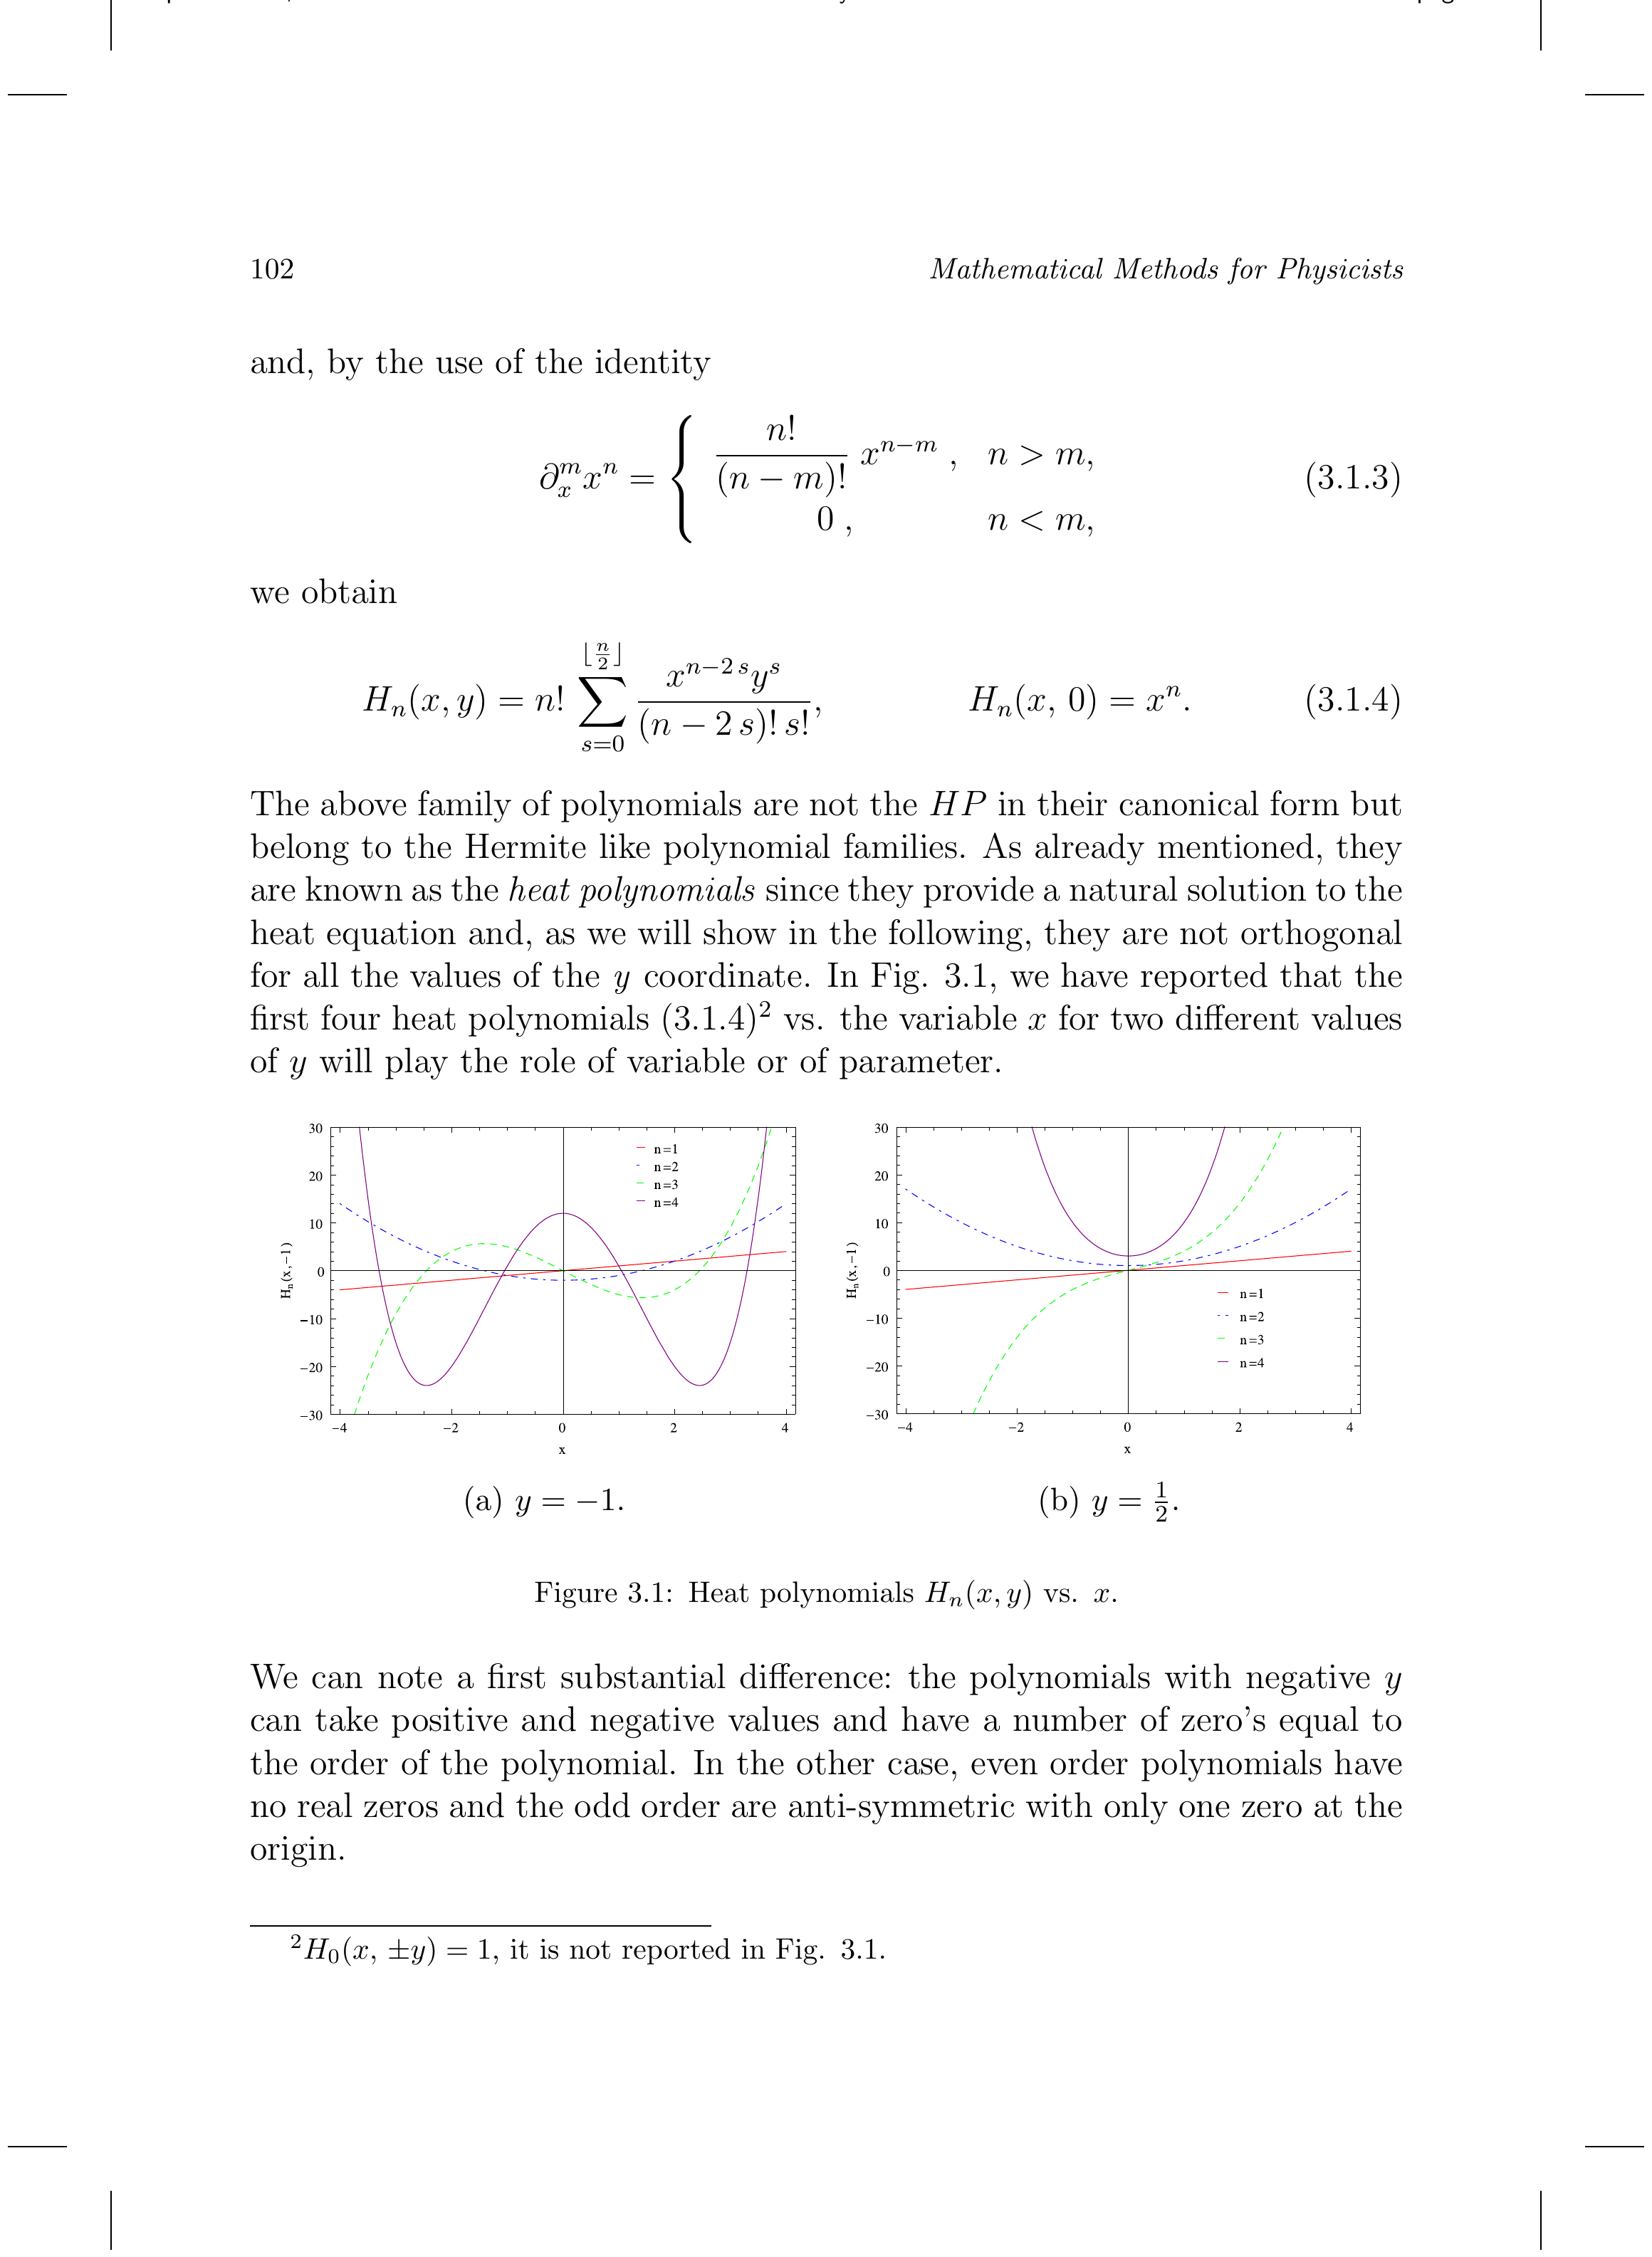
\includegraphics[max width=0.95\linewidth,keepaspectratio]{fig3_1.png}\caption{热多项式 $H_n(x,y)$ 关于变量 $x$ 的图形：(a)~$y=-1$ 与 (b)~$y=+1$。}
\label{fig:3.1}
\end{figure}

我们可以注意到第一个实质性的差异：$y$ 取负值时多项式可正可负，零点的数目等于多项式的阶数。而在另一种情形，偶阶多项式没有实零点，奇阶多项式是反对称的，只在原点有一个零点。

\medskip
算子定义~\eqref{eq:3.1.1} 极大地简化了 HP 及其推广的性质研究。由此定义显然有
\[
H_{n+1}(x,y)=e^{y\partial_x^2}(x^{n+1})
=e^{y\partial_x^2}\,x\,e^{-y\partial_x^2}\,e^{y\partial_x^2}(x^n)
=e^{y\partial_x^2}\,x\,e^{-y\partial_x^2}\,H_n(x,y).
\]
考虑到式~\eqref{eq:2.4.16}，
\[
e^{y\partial_x^2}\,x\,e^{-y\partial_x^2}=x+2y\partial_x,
\]
我们得到递推关系
\begin{equation}
H_{n+1}(x,y)=x\,H_n(x,y)+2y\,\partial_x H_n(x,y).
\label{eq:3.1.7}
\end{equation}
用类似的方法可以得到递推关系
\begin{equation}
\partial_x H_n(x,y)=n\,H_{n-1}(x,y).
\label{eq:3.1.8}
\end{equation}
这两个递推关系可以结合起来证明热多项式满足如下 ODE
\begin{equation}
2y\,z_{xx}+x\,z_x=n\,z,\qquad z=H_n(x,y).
\label{eq:3.1.9}
\end{equation}
在上述方程中，求导是对 $x$ 进行的，$y$ 被视为参数。

同样容易验证，若把 $y$ 视为变量，下列关系成立：
\begin{equation}
\partial_y H_n(x,y)=n(n-1)\,H_{n-2}(x,y).
\label{eq:3.1.10}
\end{equation}

为了把上述结果置于更一般的背景下，我们引入\emph{拟单项式}（quasi-monomial）的概念：那些可以为其定义一对算子 $\hat P$ 与 $\hat M$（分别称为求导算子与乘法算子），使得
\begin{equation}
\hat P\,p_n(x)=n\,p_{n-1}(x),\qquad
\hat M\,p_n(x)=p_{n+1}(x).
\label{eq:3.1.11}
\end{equation}
成立的多项式族 $p_n(x)$。此外，若再加上条件
\begin{equation}
p_0(x)=1,
\label{eq:3.1.12}
\end{equation}
我们就可以只用乘法算子构造拟单项式族，根据恒等式
\begin{equation}
\hat M^n\,1=p_n(x).
\label{eq:3.1.13}
\end{equation}
它由式~\eqref{eq:3.1.11} 第二个等式迭代得到。此外，若算子 $\hat M$ 与 $\hat P$ 具有微分实现，则容易证明多项式 $p_n(x)$ 满足微分方程
\begin{equation}
\hat M\hat P\,p_n(x)=n\,p_n(x).
\label{eq:3.1.14}
\end{equation}

下面，我们将讨论从普通单项式 $x^n$ 出发构造拟单项式的一般程序，其乘法算子与求导算子分别为 $x$ 与普通求导。显然，按上述定义，$H_n(x,y)$ 是拟单项式，其乘法算子与求导算子可以确定为
\begin{equation}
\hat M=x+2y\partial_x,\qquad \hat P=\partial_x
\label{eq:3.1.15}
\end{equation}
以及
\begin{equation}
\hat M\hat P=x\partial_x+2y\partial_x^2.
\label{eq:3.1.16}
\end{equation}
因此，HP 是算子~\eqref{eq:3.1.16} 的（实）特征值 $n$ 的本征函数。

\noindent{\itshape 注记.} 在此情形下，$y$ 应视为参数而非变量。应当使用全导数记号，但为记号连续性我们使用偏导数。

以上引言性评注构成了后续各节讨论的骨架。

% ------------------------------------------------------------------
\section{Hermite 多项式的生成函数}
\label{sec:3.2}

\subsection{引入生成函数}
\label{sec:3.2.1}

由于多项式 $H_n(x,y)$ 是热方程的解，它们可以通过含二阶导数算子的演化算子的算子定义引入。下列两个重要恒等式是该定义的直接结果：
\begin{equation}
e^{z\partial_x^2}H_n(x,y)=H_n(x,y+z),\qquad
e^{-y\partial_x^2}H_n(x,y)=x^n.
\label{eq:3.2.1}
\end{equation}
它们虽然直接，却非常重要，应当仔细考虑。

Hermite（热）多项式的另一个重要性质是生成函数，它将在后文被广泛使用。所谓给定多项式族 $p_n(x)$ 的生成函数，指的是函数
\begin{equation}
G(x,t)=\sum_{n=0}^{\infty}\frac{t^n}{n!}\,p_n(x)
\label{eq:3.2.2}
\end{equation}
它本质上是变量 $t$ 与 $x$ 的函数。对 $t$（称为生成函数的展开变量）作 Taylor 展开，系数 $\partial_t^n G(x,t)|_{t=0}$ 正是多项式 $p_n(x)$。显然普通单项式由
\begin{equation}
\sum_{n=0}^{\infty}\frac{t^n}{n!}\,x^n=e^{xt}.
\label{eq:3.2.3}
\end{equation}
生成。

根据式~\eqref{eq:3.1.1}，我们可以把 HP 的生成函数定义为
\[
\sum_{n=0}^{\infty}\frac{t^n}{n!}\,H_n(x,y)
=e^{y\partial_x^2}\!\left(\sum_{n=0}^{\infty}\frac{t^n}{n!}\,x^n\right)
=e^{y\partial_x^2}\,e^{xt}.
\]
利用 $e^{y\partial_x^2}\,e^{xt}=e^{xt+yt^2}$（因为 $\partial_x^m e^{xt}=t^m e^{xt}$），得到
\begin{equation}
\sum_{n=0}^{\infty}\frac{t^n}{n!}\,H_n(x,y)=e^{xt+yt^2}.
\label{eq:3.2.5}
\end{equation}

\noindent{\itshape 注记.} 应当注意，一般有 $e^{2yt\partial_x}\neq 1$，因此中间步骤需要算子解缠
$e^{y\partial_x^2}\,e^{xt}=e^{yt^2}\,e^{xt}\,e^{2yt\partial_x}$，随后作用于真空 $1$。

\medskip
正如后文将展示的，这是 Hermite 多项式理论中一个极其重要的关系。

我们作为算子形式体系的副产品、并在陈述了这一多项式族的主要性质之后推导出了 HP 的生成函数。在更经典的特殊函数教材中，HP 的显式形式直接由生成函数推得。为理解这一程序，我们回顾级数乘积的 Cauchy 公式：给定两个无穷级数
\[
S_1=\sum_{s=0}^{\infty}b_s\,x^s,\qquad
S_2=\sum_{r=0}^{\infty}a_r\,x^r,
\]
我们得到
\[
S_1S_2=\sum_{s=0}^{\infty}\sum_{r=0}^{\infty}b_s\,a_r\,x^{r+s}
=\sum_{n=0}^{\infty}c_n\,x^n,\qquad
c_n=\sum_{r=0}^{n}a_r\,b_{n-r}.
\]

因此，我们可以直接从生成函数~\eqref{eq:3.2.5} 推出 HP：
\[
e^{xt+yt^2}=e^{xt}\,e^{yt^2}
=\sum_{r=0}^{\infty}\frac{x^r t^r}{r!}
 \sum_{s=0}^{\infty}\frac{y^s t^{2s}}{s!}
=\sum_{n=0}^{\infty}\frac{t^n}{n!}\,H_n(x,y),
\]
并令 $r+2s=n$，根据定义~\eqref{eq:3.1.4}，得到
\[
\sum_{n=0}^{\infty}\frac{t^n}{n!}\,H_n(x,y)
=e^{xt+yt^2}.
\]

\subsection{生成函数的应用}
\label{sec:3.2.2}

形如
\begin{equation}
I_n(a,b)=\int_{-\infty}^{\infty}(x+b)^n\,e^{-ax^2}\,dx
\label{eq:3.2.11}
\end{equation}
的积分在物理或工程问题的求解中经常出现。用生成函数方法计算这些积分非常高效。若我们注意到
\[
\sum_{n=0}^{\infty}\frac{t^n}{n!}\,I_n(a,b)
=\int_{-\infty}^{\infty}e^{tb}\,e^{tx}\,e^{-ax^2}\,dx
=e^{tb}\,\sqrt{\frac{\pi}{a}}\;e^{\frac{t^2}{4a}},
\label{eq:3.2.12}
\]
根据式~\eqref{eq:3.2.5}，并对式~\eqref{eq:3.2.12} 应用多项式恒等原理（即令同幂次的 $t$ 相等），我们得到如下结果
\begin{equation}
I_n(a,b)=\sqrt{\frac{\pi}{a}}\;\frac{1}{a^{n/2}}\,
H_n\!\left(\frac{b}{\sqrt{a}},\frac{1}{4a}\right).
\label{eq:3.2.13}
\end{equation}

另外两个性质
\begin{equation}
\partial_x^n e^{ax^2}=H_n(2ax,a)\,e^{ax^2},
\label{eq:3.2.14}
\end{equation}
\begin{equation}
a^n H_n(x,y)=H_n(ax,a^2y),
\label{eq:3.2.15}
\end{equation}
可以用生成函数方法证明。式~\eqref{eq:3.2.14} 确实是平移算子性质的直接结果：
\[
\sum_{n=0}^{\infty}\frac{t^n}{n!}\,\partial_x^n e^{ax^2}
=e^{t\partial_x}e^{ax^2}=e^{a(x+t)^2}
=e^{ax^2}\,e^{2atx+at^2}
=e^{ax^2}\sum_{n=0}^{\infty}\frac{t^n}{n!}\,H_n(2ax,a),
\]
而式~\eqref{eq:3.2.15} 留作练习。

\noindent{\itshape 注记.} 注意，式~\eqref{eq:3.2.15} 的一个重要推论是恒等式
$(-1)^n H_n(x,y)=H_n(-x,y)$。

\medskip
作为生成函数方法应用的又一例，我们考虑下列定理的证明。

\begin{theorem}[加法]
$\forall\,x,y,z\in\mathbb{R},\;\forall n\in\mathbb{N}$
\begin{equation}
H_n(x+z,y)=\sum_{s=0}^{n}\binom{n}{s}\,
H_{n-s}\!\left(x,\frac{y}{2}\right)
H_s\!\left(z,\frac{y}{2}\right).
\label{eq:3.2.17}
\end{equation}
\end{theorem}

\noindent{\itshape 提示：}它只是下列事实的推论：
\[
\sum_{n=0}^{\infty}\frac{t^n}{n!}\,H_n(x+z,y)
=e^{(x+z)t+yt^2}
=e^{xt+yt^2/2}\;e^{zt+yt^2/2}.
\tag{3.2.18}
\]

下面这个问题极其重要，因为它涉及一个非平凡的排序问题，并让我们看到 HP 如何非常自然地在处理含乘法求导算子的表达式中出现。问题在于求算子
\begin{equation}
\hat O_n=(\alpha\partial_x+\beta x)^n.
\label{eq:3.2.19}
\end{equation}
的 Newton 二项式形式的类比。

根据前面的讨论，我们有
\[
\sum_{n=0}^{\infty}\frac{t^n}{n!}\,\hat O_n
=e^{t(\alpha\partial_x+\beta x)}
=e^{\beta t x+\frac{\alpha\beta}{2}t^2}\;e^{\alpha t\partial_x},
\]
再考虑到式~\eqref{eq:3.2.5}，可以写出
\[
e^{\beta t x+\frac{\alpha\beta}{2}t^2}
=\sum_{r=0}^{\infty}\frac{t^r}{r!}\,
H_r\!\left(\beta x,\frac{\alpha\beta}{2}\right)
=\sum_{r=0}^{\infty}\frac{t^r}{r!}\,H_r\!\left(\beta x,\frac{\alpha\beta}{2}\right)
 \sum_{s=0}^{\infty}\frac{(\alpha t)^s}{s!}\,\partial_x^s,
\]
应用 Cauchy 乘积公式并与 $\sum t^n\hat O_n/n!$ 比较，得到
\begin{equation}
\hat O_n=\sum_{s=0}^{n}\frac{1}{s!}\,
\alpha^s\,H_{n-s}\!\left(\beta x,\frac{\alpha\beta}{2}\right)\,\partial_x^s,
\label{eq:3.2.22}
\end{equation}
这是所谓\emph{Burchnall} 算子规则的推广，可用于证明恒等式
\begin{equation}
\hat O_n\,e^{-x^2}
=\sum_{s=0}^{n}\frac{(-\alpha)^s}{s!}\,
H_{n-s}\!\left(\beta x,\frac{\alpha\beta}{2}\right)
H_s(2x,-1)\,e^{-x^2}
=H_n\!\left((\beta-2\alpha)x,\frac{\alpha(\beta-2\alpha)}{2}\right)e^{-x^2}.
\label{eq:3.2.23}
\end{equation}

我们将在本书第二部分讨论生成函数方法应用的更多例子。

% ------------------------------------------------------------------
\section{Hermite 多项式作为正交基}
\label{sec:3.3}

我们将在稍后更仔细地定义正交多项式的概念。这里我们讨论以下问题：给定关于 $x$ 的函数在什么条件下可以按 Hermite 多项式展开？

为此，我们把第二变量 $y$ 视为参数，并限于 $y<0$ 的情形。因此我们写出
\begin{equation}
F(x)=\sum_{n=0}^{\infty}a_n\,H_n(x,-|y|).
\label{eq:3.3.1}
\end{equation}
现在的任务是计算上述展开的系数 $a_n$。根据定义~\eqref{eq:3.1.1}，我们可以把~\eqref{eq:3.3.1} 改写为
\[
F(x)=e^{-|y|\partial_x^2}\!\left(\sum_{n=0}^{\infty}a_n\,x^n\right),
\]
求逆得到
\[
\Phi(x)\equiv e^{|y|\partial_x^2}\!\bigl(F(x)\bigr)
=\sum_{n=0}^{\infty}a_n\,x^n.
\]
根据 Gauss--Weierstrass 变换（见式~\eqref{eq:2.2.17}），函数 $\Phi(x)$ 有下列积分表示：
\begin{equation}
\Phi(x)=\frac{1}{\sqrt{4\pi|y|}}\int_{-\infty}^{\infty}
e^{-\frac{(x-\sigma)^2}{4|y|}}\,F(\sigma)\,d\sigma.
\label{eq:3.3.4}
\end{equation}
利用 HP 的生成函数，最后一个恒等式可以写成
\[
\Phi(x)=\frac{1}{\sqrt{4\pi|y|}}
 \sum_{n=0}^{\infty}\frac{1}{n!}
 \int_{-\infty}^{\infty}
 H_n\!\left(\frac{\sigma}{2\sqrt{|y|}},-\frac{1}{4}\right)
 e^{-\frac{(x-\sigma)^2}{4|y|}}\,F(\sigma)\,d\sigma,
\]
与 $\Phi(x)=\sum a_n x^n$ 比较，给出系数 $a_n$ 的表达式
\begin{equation}
a_n=\frac{1}{2^n n!\sqrt{\pi|y|}}
\int_{-\infty}^{\infty}
H_n\!\left(\frac{\sigma}{2\sqrt{|y|}},-\frac{1}{4}\right)
e^{-\frac{\sigma^2}{4|y|}}\,F(\sigma)\,d\sigma.
\label{eq:3.3.6}
\end{equation}

我们指出，作为式~\eqref{eq:3.3.1} 的推论，函数
\begin{equation}
\phi_n(x)=\frac{1}{\sqrt{2^n n!\,\pi|y|}}\,
H_n\!\left(\frac{x}{2\sqrt{|y|}},-\frac{1}{4}\right)
e^{-\frac{x^2}{4|y|}}
\label{eq:3.3.7}
\end{equation}
与 Hermite 多项式 $H_n(x,-|y|)$ 双正交（bi-orthogonal）。用更常规的说法，可以表述为：多项式 $H_n\!\left(\frac{x}{2\sqrt{|y|}},-\frac{1}{4}\right)$ 以权重函数 $e^{-x^2/(4|y|)}$ 与 $H_n(x,-|y|)$ 正交。HP 的规范形式取 $|y|=1/2$，记作 $\mathrm{He}_n(x)$，即
\begin{equation}
\mathrm{He}_n(x)=H_n\!\left(x,-\frac{1}{2}\right).
\label{eq:3.3.8}
\end{equation}
在应用中，也使用形式
\begin{equation}
H_n(x)=H_n(2x,-1)=2^n H_n\!\left(x,-\frac{1}{4}\right)
\label{eq:3.3.9}
\end{equation}
我们两种记号都会采用。这两种形式由恒等式
\begin{equation}
H_n(x)=2^{n/2}\,\mathrm{He}_n\!\left(\frac{x}{\sqrt{2}}\right).
\label{eq:3.3.10}
\end{equation}
联系。

此外，$H_n(x,y)$ 与 Hermite 规范形式的联系由下式给出
\begin{equation}
H_n(x,y)=(-i)^n\,y^{n/2}\,
H_n\!\left(\frac{x}{2\sqrt{-y}}\right)
=2^n\,(-iy)^{n/2}\,
\mathrm{He}_n\!\left(\frac{x}{2\sqrt{-iy}}\right).
\label{eq:3.3.11}
\end{equation}

不难验证，上述关系是前面概述性质的直接推论。

\noindent{\itshape 注记.} 两组函数 $\gamma_n(x)$、$\lambda_n(x)$ 称为\emph{双正交}的，如果
$\int \gamma_n(x)\,\lambda_m(x)\,dx=\delta_{nm}$。例如在区间 $[0,2\pi]$ 上 $\sin(nx)$、$\cos(mx)$ 是双正交的。

\medskip
现在推导函数~\eqref{eq:3.3.7} 满足的微分方程。它将通过一个简单而有效的方法确定。由式~\eqref{eq:3.3.7}，有
\[
H_n\!\left(\frac{x}{2\sqrt{|y|}},-\frac{1}{4}\right)
=A_n\,e^{\frac{x^2}{4|y|}}\,\phi_n(x),\qquad
A_n=\sqrt{2^n n!\,\pi|y|}.
\]

在算子语言中，确定多项式 $H_n(x,y)$ 微分方程的 ODE 可以写成（见式~\eqref{eq:3.1.14} 与~\eqref{eq:3.1.16}）
\[
\hat h_{\mathrm{er}}\,H_n(ax,y)=0,\qquad
\hat h_{\mathrm{er}}=\partial_x^2+a^2x\partial_x-n a^2.
\]
将算子 $\hat h_{\mathrm{er}}$ 作用于式~\eqref{eq:3.3.7}，得到
\[
\left(-2|y|\partial_x^2+x\partial_x-n\right)e^{\frac{x^2}{4|y|}}\phi_n(x)=0,
\]
于是对 $\phi_n(x)$，我们得到具有非常数系数的二阶微分方程
\begin{equation}
\left(-2|y|\partial_x^2-x\partial_x-1\right)\phi_n(x)=n\,\phi_n(x).
\label{eq:3.3.15}
\end{equation}
这一结果意味着函数 $\phi_n$ 是算子
\begin{equation}
\hat\eta_{\mathrm{her}}=-2|y|\partial_x^2-x\partial_x-1,
\label{eq:3.3.16}
\end{equation}
的以 $n$ 为特征值的本征函数，当 $y<0$ 时，该算子是式~\eqref{eq:3.1.16} 中算子的厄米共轭。

\noindent{\itshape 注记.} 我们提醒，两个算子乘积的厄米共轭是
$(\hat A\hat B)^\dagger=\hat B^\dagger\hat A^\dagger$，且由 $\hat x^\dagger=\hat x$ 与 $\partial_x^\dagger=-\partial_x$，可得
$(x\partial_x)^\dagger=-\partial_x x\ldots$

\medskip
虽然不作证明，我们强调如下命题。

\begin{proposition}
互为厄米共轭的两个算子的本征函数构成一个双正交集。
\end{proposition}

现在考虑 $y=-1/2$ 时规范 Hermite 多项式的情形，定义函数
\begin{equation}
\Phi_n(x)=\alpha_n\,\mathrm{He}_n(x)\,e^{-x^2/4}.
\label{eq:3.3.17}
\end{equation}
它显然提供一个正交函数集，其归一化常数 $\alpha_n$ 稍后确定。函数~\eqref{eq:3.3.17} 满足的微分方程可以按照前面说明函数~\eqref{eq:3.3.7} 的方法得到，即若令
\[
\phi_n(x)=\Phi_n(x)\,e^{x^2/4}.
\]
根据式~\eqref{eq:3.3.15}，函数 $\Phi_n(x)$ 满足的 ODE 是
\begin{equation}
\left(\frac{x^2}{4}-\partial_x^2-\frac{1}{2}\right)\Phi_n(x)
=n\,\Phi_n(x),
\label{eq:3.3.19}
\end{equation}
这正是量子谐振子方程。谐振子本征函数通常写在基 $H_n(x)$ 下，为
\begin{equation}
\Phi_n(x)=\frac{1}{\sqrt{2^n n!\sqrt{\pi}}}\,
H_n(x)\,e^{-x^2/2}.
\label{eq:3.3.20}
\end{equation}

\begin{exercise}
证明式~\eqref{eq:3.3.20} 给出一个标准正交集，即 $\Phi_n(x)$ 相互正交且归一化到 1。
\end{exercise}

在图~\ref{fig:3.2} 中我们给出了前六个谐振子本征函数的行为。

\begin{figure}[H]
\centering
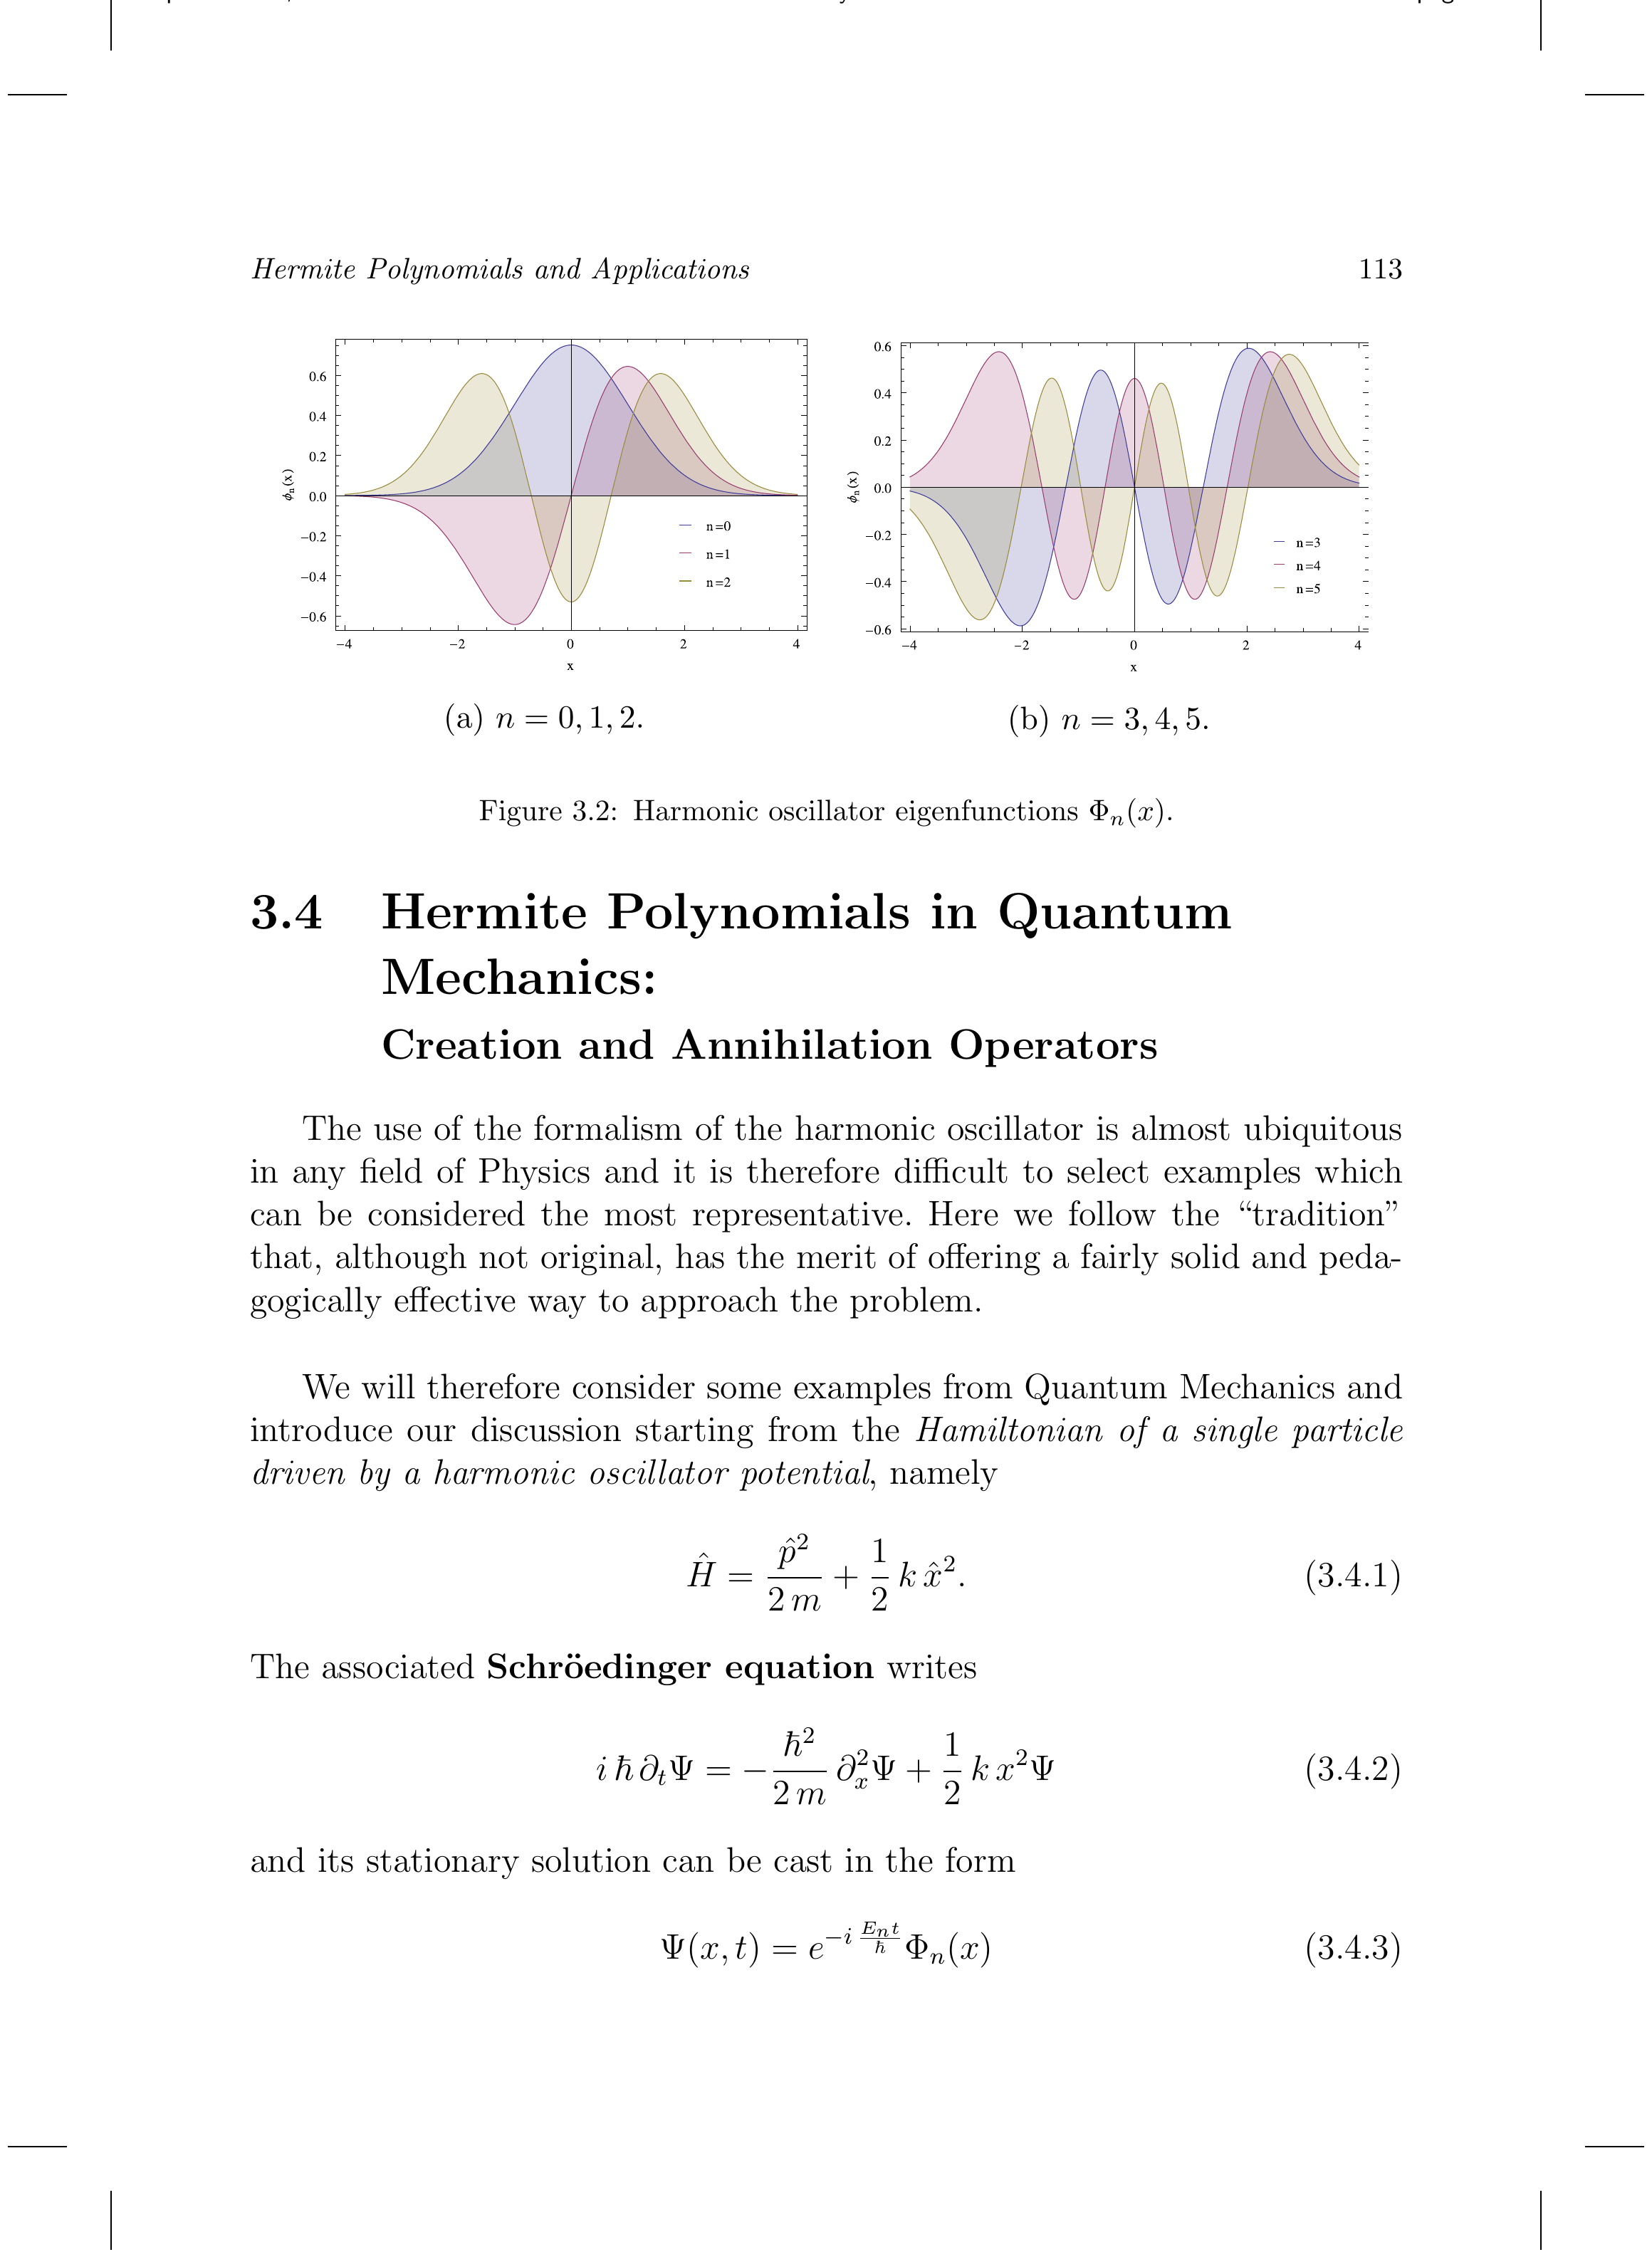
\includegraphics[max width=0.95\linewidth,keepaspectratio]{fig3_2.png}\caption{谐振子本征函数 $\Phi_n(x)$。}
\label{fig:3.2}
\end{figure}

函数按 HP 的展开将在练习与补充部分讨论。这里我们给出这种展开的一个非常简单但重要的例子。

\begin{exercise}
证明
\begin{equation}
x^n=\sum_{s=0}^{\lfloor n/2\rfloor}
\frac{n!}{s!\,(n-2s)!}\,(-1)^s\,y^s\,H_{n-2s}(x,y).
\tag{3.3.21}
\end{equation}
\noindent{\itshape 提示：}使用生成函数方法，注意 $e^{xt}=e^{xt+yt^2-yt^2}$。
\end{exercise}

% ------------------------------------------------------------------
\section{量子力学中的 Hermite 多项式：产生与湮灭算子}
\label{sec:3.4}

谐振子形式体系的使用几乎遍及物理学的所有领域，因此很难选出最具代表性的例子。这里我们遵循``传统''做法，它虽然并不原创，但具有提供一种相当扎实、教学上有效的方法来切入问题的优点。

因此，我们将考虑量子力学中的若干例子，并从受谐振子势驱动的单粒子哈密顿量开始，即
\begin{equation}
\hat H=\frac{\hat p^2}{2m}+\frac{1}{2}\,k\,\hat x^2.
\label{eq:3.4.1}
\end{equation}
相应的 Schr\"odinger 方程为
\begin{equation}
i\hbar\,\partial_t\Psi=-\frac{\hbar^2}{2m}\,\partial_x^2\Psi
+\frac{1}{2}\,k\,x^2\Psi
\label{eq:3.4.2}
\end{equation}
其定态解可以写成
\begin{equation}
\Psi(x,t)=e^{-iE_n t/\hbar}\,\Phi_n(x).
\label{eq:3.4.3}
\end{equation}

\begin{figure}[H]
\centering
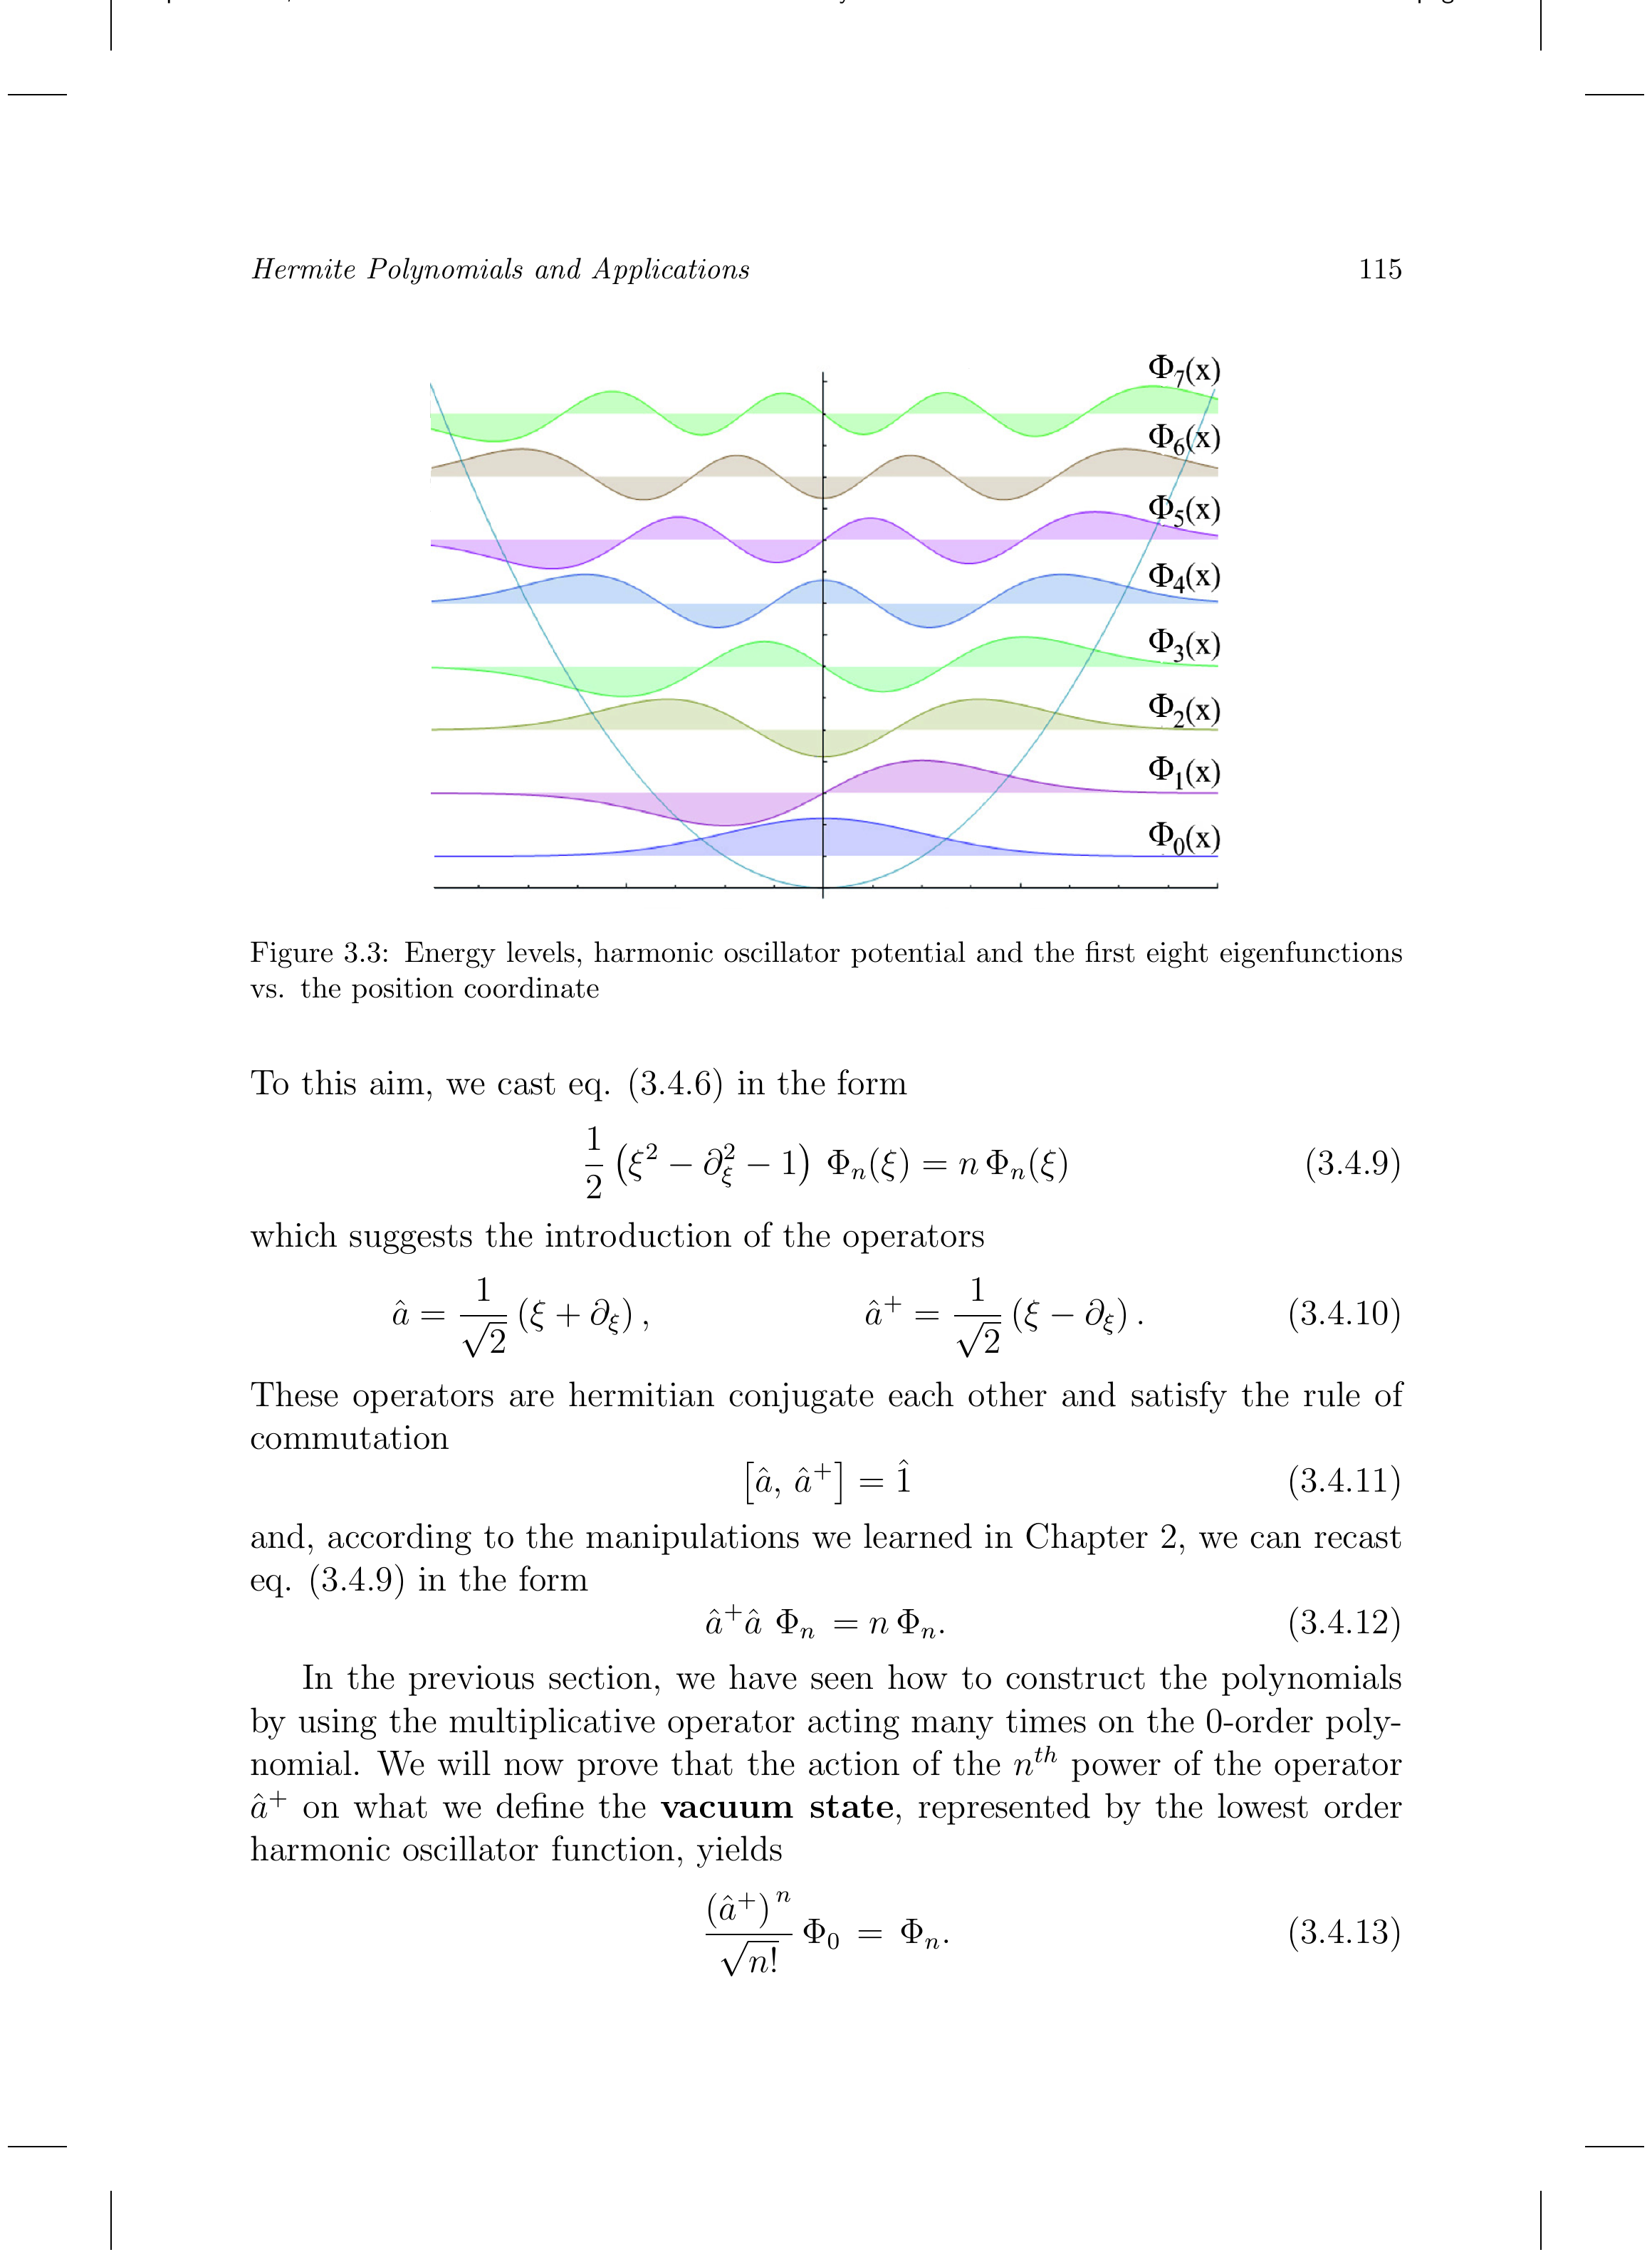
\includegraphics[max width=0.95\linewidth,keepaspectratio]{fig3_3.png}\caption{能级、谐振子势与前八个本征函数关于位置坐标的图形。}
\label{fig:3.3}
\end{figure}

代入式~\eqref{eq:3.4.2}，得到
\begin{equation}
E_n\,\Phi_n(x)=-\frac{\hbar^2}{2m}\,\partial_x^2\Phi_n(x)
+\frac{1}{2}\,k\,x^2\Phi_n(x),
\label{eq:3.4.4}
\end{equation}
其中 $\omega=\sqrt{k/m}$ 是我们问题的特征频率。式~\eqref{eq:3.4.4} 正是谐振子本征函数满足的 ODE（注意这里指基 $H_n(x)$ 下的本征函数）。我们指出，量
\begin{equation}
x_q\equiv\sqrt{\frac{\hbar}{m\omega}}
\label{eq:3.4.5}
\end{equation}
具有长度的量纲（其物理意义将在下面讨论），把式~\eqref{eq:3.4.4} 用变量 $\xi=x/x_q$ 改写，得到
\begin{equation}
E_n\,\Phi_n(\xi)=-\frac{\hbar\omega}{2}\,\partial_\xi^2\Phi_n(\xi)
+\frac{\hbar\omega}{2}\,\xi^2\Phi_n(\xi),
\label{eq:3.4.6}
\end{equation}
能量本征值 $E_n$ 可以用特征频率写成
\begin{equation}
E_n=\hbar\omega\!\left(n+\frac{1}{2}\right).
\label{eq:3.4.7}
\end{equation}

在图~\ref{fig:3.3} 中，我们给出了二次势、能级与前八个波函数。显然激发阶数越大，分布函数的空间延展越大。必须强调，0 阶本征函数（即最低能级）为
\[
\Phi_0(x)\propto e^{-x^2/(2x_q^2)},
\]
即一个均方根（r.m.s.）与 $x_q$ 成正比的波包。

在前面的讨论中，我们引入了弹性常数 $k$，它是最重要的物理参数，因为它确定了振荡频率，从而确定了能量本征值之间的间隔。我们将在下一节讨论涉及具体应用的例子，如双原子分子。这里我们继续确定后面将使用的形式体系，即引入产生--湮灭算子。

为此，把式~\eqref{eq:3.4.6} 改写为
\begin{equation}
\left(\xi^2-\partial_\xi^2-1\right)\Phi_n(\xi)=2n\,\Phi_n(\xi),
\label{eq:3.4.9}
\end{equation}
这提示引入算子
\begin{equation}
\hat a=\frac{1}{\sqrt{2}}\,(\xi+\partial_\xi),\qquad
\hat a^\dagger=\frac{1}{\sqrt{2}}\,(\xi-\partial_\xi).
\label{eq:3.4.10}
\end{equation}
这两个算子互为厄米共轭，满足对易规则
\begin{equation}
[\hat a,\hat a^\dagger]=\hat 1.
\label{eq:3.4.11}
\end{equation}
并且，根据我们在第 2 章学到的运算技巧，可以把式~\eqref{eq:3.4.9} 改写为
\begin{equation}
\hat a^\dagger\hat a\,\Phi_n(\xi)=n\,\Phi_n(\xi).
\label{eq:3.4.12}
\end{equation}

在上一节中，我们看到如何通过乘法算子多次作用于 0 阶多项式来构造多项式。我们现在将证明，算子 $\hat a^\dagger$ 的 $n$ 次幂作用于我们所定义的真空态（由最低阶谐振子函数代表）的结果为
\begin{equation}
\frac{(\hat a^\dagger)^n}{\sqrt{n!}}\,\Phi_0=\Phi_n.
\label{eq:3.4.13}
\end{equation}

为了证明上述恒等式正确，我们使用生成函数方法，据此得到
\[
\sum_{n=0}^{\infty}\frac{t^n}{n!}\,(\hat a^\dagger)^n\Phi_0(\xi)
=e^{t\hat a^\dagger}\Phi_0(\xi)
=e^{-t^2/4}\,e^{\sqrt{t/2}\,\xi}\,
 e^{-t^2/4}\,e^{\sqrt{t/2}\,\xi}\,e^{-\xi^2/2}
\]
\begin{align*}
&=e^{-t^2/2}\,e^{\sqrt{2t}\,\xi}\,e^{-\xi^2/2}
 =\sum_{m=0}^{\infty}\frac{t^m}{m!}\,
  \mathrm{He}_m\!\left(\sqrt{2}\,\xi\right)\,e^{-\xi^2/2}.
\tag{3.4.14}
\end{align*}
比较同幂次系数，便证明了恒等式~\eqref{eq:3.4.13}，同时还得到
\begin{equation}
\hat a^\dagger\Phi_n=\sqrt{n+1}\,\Phi_{n+1}.
\label{eq:3.4.15}
\end{equation}
因此，我们称 $\hat a^\dagger$ 为``产生''算子。类似地，``湮灭''算子的伴随恒等式也可以用同样的方法验证：
\begin{equation}
\hat a\,\Phi_n=\sqrt{n}\,\Phi_{n-1}.
\label{eq:3.4.16}
\end{equation}

这样我们就证明了三个算子在量子谐振子动力学中起基本作用：互为厄米共轭的产生--湮灭对（有时称为升降算子），以及称为数算子的厄米算子 $\hat a^\dagger\hat a$。

Dirac 记号常被用来描述谐振子态。确实有对应关系
\begin{equation}
|0\rangle\to\Phi_0(\xi),\qquad
|n\rangle\to\Phi_n(\xi)
\label{eq:3.4.17}
\end{equation}
正交性可以表示为
\begin{equation}
\langle m|n\rangle=\delta_{m,n}.
\label{eq:3.4.18}
\end{equation}

在式~\eqref{eq:3.4.17} 中，我们把表示所谓真空态的 $|0\rangle$ 态单独列出。更严格地说，Dirac 记号（也称 $n$ 态）与谐振子本征函数之间的对应应当写成
\begin{equation}
\langle \xi|n\rangle=\Phi_n(\xi).
\label{eq:3.4.19}
\end{equation}

问题的这一方面将在本书第二部分引入所谓相干态时更仔细地讨论。

% ------------------------------------------------------------------
\section{量子力学应用}
\label{sec:3.5}

遗憾的是，我们无法深入讨论上述形式体系在量子力学问题中的应用，因此我们将局限于几个能说明其强大与优雅的例子。我们要讨论的第一个问题是受谐振子势支配并处于经典电场作用下的带电粒子。

相关哈密顿量可以写成
\begin{equation}
\hat H=\frac{\hat p^2}{2m}+\frac{1}{2}\,k\,\hat x^2-eE\hat x,
\label{eq:3.5.1}
\end{equation}
其中电场 $E$ 恒定且均匀，即它与时间和坐标无关。与我们已研究情形的差别在于存在一个线性的势，它体现了电场的作用。

上述问题可以通过把哈密顿量改写为
\begin{equation}
\hat H=\frac{\hat p^2}{2m}+\frac{1}{2}\,m\omega^2
\left(\hat x-\frac{eE}{m\omega^2}\right)^2\hat 1
-\frac{(eE)^2}{2m\omega^2}\,\hat 1.
\label{eq:3.5.2}
\end{equation}
而轻松地转化为普通谐振子问题。式~\eqref{eq:3.5.2} 中最后一项乘以单位算子后是一个具有能量量纲的常数，而
\begin{equation}
x_s\equiv\frac{eE}{m\omega^2}
\label{eq:3.5.3}
\end{equation}
是电场引起的坐标平移。由于电场恒定且均匀，把哈密顿量整理成形如~\eqref{eq:3.5.2} 的形式提示我们引入坐标算子
\begin{equation}
\hat X=\hat x-\frac{eE}{m\omega^2}\,\hat 1
\label{eq:3.5.4}
\end{equation}
它不改变我们问题的对易关系，且
\begin{equation}
[\hat p,\hat X]=-i\hbar\,\hat 1.
\label{eq:3.5.5}
\end{equation}
因此可以得出如下结论：
\begin{enumerate}
\item 能量本征值与之前相同，但增加了一项由电场效应引起的项，即
      \begin{equation}
      E_n=\hbar\omega\!\left(n+\frac{1}{2}\right)-\frac{(eE)^2}{2m\omega^2}.
      \label{eq:3.5.6}
      \end{equation}
\item 本征函数保持不变，但自变量应替换为
      \begin{equation}
      \xi\to\xi-\xi_0,\qquad
      \xi_0=\frac{x_s}{x_q}=\sqrt{\frac{2}{m\hbar\omega}}\;eE.
      \label{eq:3.5.7}
      \end{equation}
\end{enumerate}

我们要讨论的第二个例子是 Landau 能级，它出现在电子（或任何带电粒子）在经典磁场中运动的量子分析中。支配该过程的哈密顿算子可以写成（cgs 单位制）
\begin{equation}
\hat H=\frac{1}{2m}\left(\hat{\vec p}-\frac{q}{c}\,\vec A\right)^2.
\label{eq:3.5.8}
\end{equation}
其中 $\vec A$ 是矢势。假定磁场沿 $z$ 方向，且电子在 $x,y$ 平面内运动，
\begin{equation}
\vec B=\nabla\times\vec A,
\label{eq:3.5.9}
\end{equation}
我们可以把 $\vec A$ 写成
\begin{equation}
\vec A\equiv(0,Bx,0).
\label{eq:3.5.10}
\end{equation}
于是哈密顿量可以写成
\begin{equation}
\hat H=\frac{1}{2m}\left[\hat p_x^2
+\left(\hat p_y-\frac{qB}{c}\,\hat x\right)^2\right].
\label{eq:3.5.11}
\end{equation}
由于算子 $\hat p_y$ 与哈密顿量对易，可以断定沿 $y$ 方向的动量是守恒量，可以用其本征值 $\hbar k_y$ 代替。于是哈密顿量很容易被识别为与前例类似的平移谐振子哈密顿量：
\[
\hat H=\frac{\hat p_x^2}{2m}
+\frac{1}{2}\,m\omega_c^2
\left(\hat x-x_B\,\hat 1\right)^2
+\frac{\hbar^2 k_y^2}{2m},
\]
\begin{equation}
\omega_c=\frac{|q|B}{mc},\qquad x_B=\frac{\hbar c k_y}{qB}.
\label{eq:3.5.12}
\end{equation}
上述哈密顿量的本征函数可以写成
\begin{equation}
\Phi_{L,n}(x,y)=e^{ik_y y}\,\Phi_n(x-x_B),
\label{eq:3.5.13}
\end{equation}
它本质上是平面波与谐振子本征函数的乘积，而相应的本征值为
\begin{equation}
E_n=\hbar\omega_c\!\left(n+\frac{1}{2}\right)
+\frac{\hbar^2 k_y^2}{2m}.
\label{eq:3.5.14}
\end{equation}
其中频率 $\omega_c$ 称为回旋频率。

在结束对量子谐振子形式体系应用的这一概述之前，我们讨论用于处理双原子分子动力学行为的 Morse 势，以及它用谐振子势近似的做法。Morse 势能函数的形式为
\begin{equation}
V(r)=D_e\!\left(1-e^{-a(r-r_e)}\right)^2,
\label{eq:3.5.15}
\end{equation}
其中 $r$ 是原子间距离，$r_e$ 是平衡键长，$D_e$ 是阱深（相对于离解后的原子定义），$a$ 表征势的``宽度''。键的解离能可以用阱深减去零点能 $E(0)$ 得到。把 $V(r)$ 对 $(r-r_e)$ 展开到最低阶，得到
\begin{equation}
V(r)\approx\frac{a^2D_e}{2}\,(r-r_e)^2.
\label{eq:3.5.16}
\end{equation}
因此可以令 $a^2D_e/2=\frac{1}{2}k$，把该近似解释为谐振子势。Morse 势（蓝色）与谐振子势（绿色）的比较见图~\ref{fig:3.4}。

\begin{figure}[H]
\centering
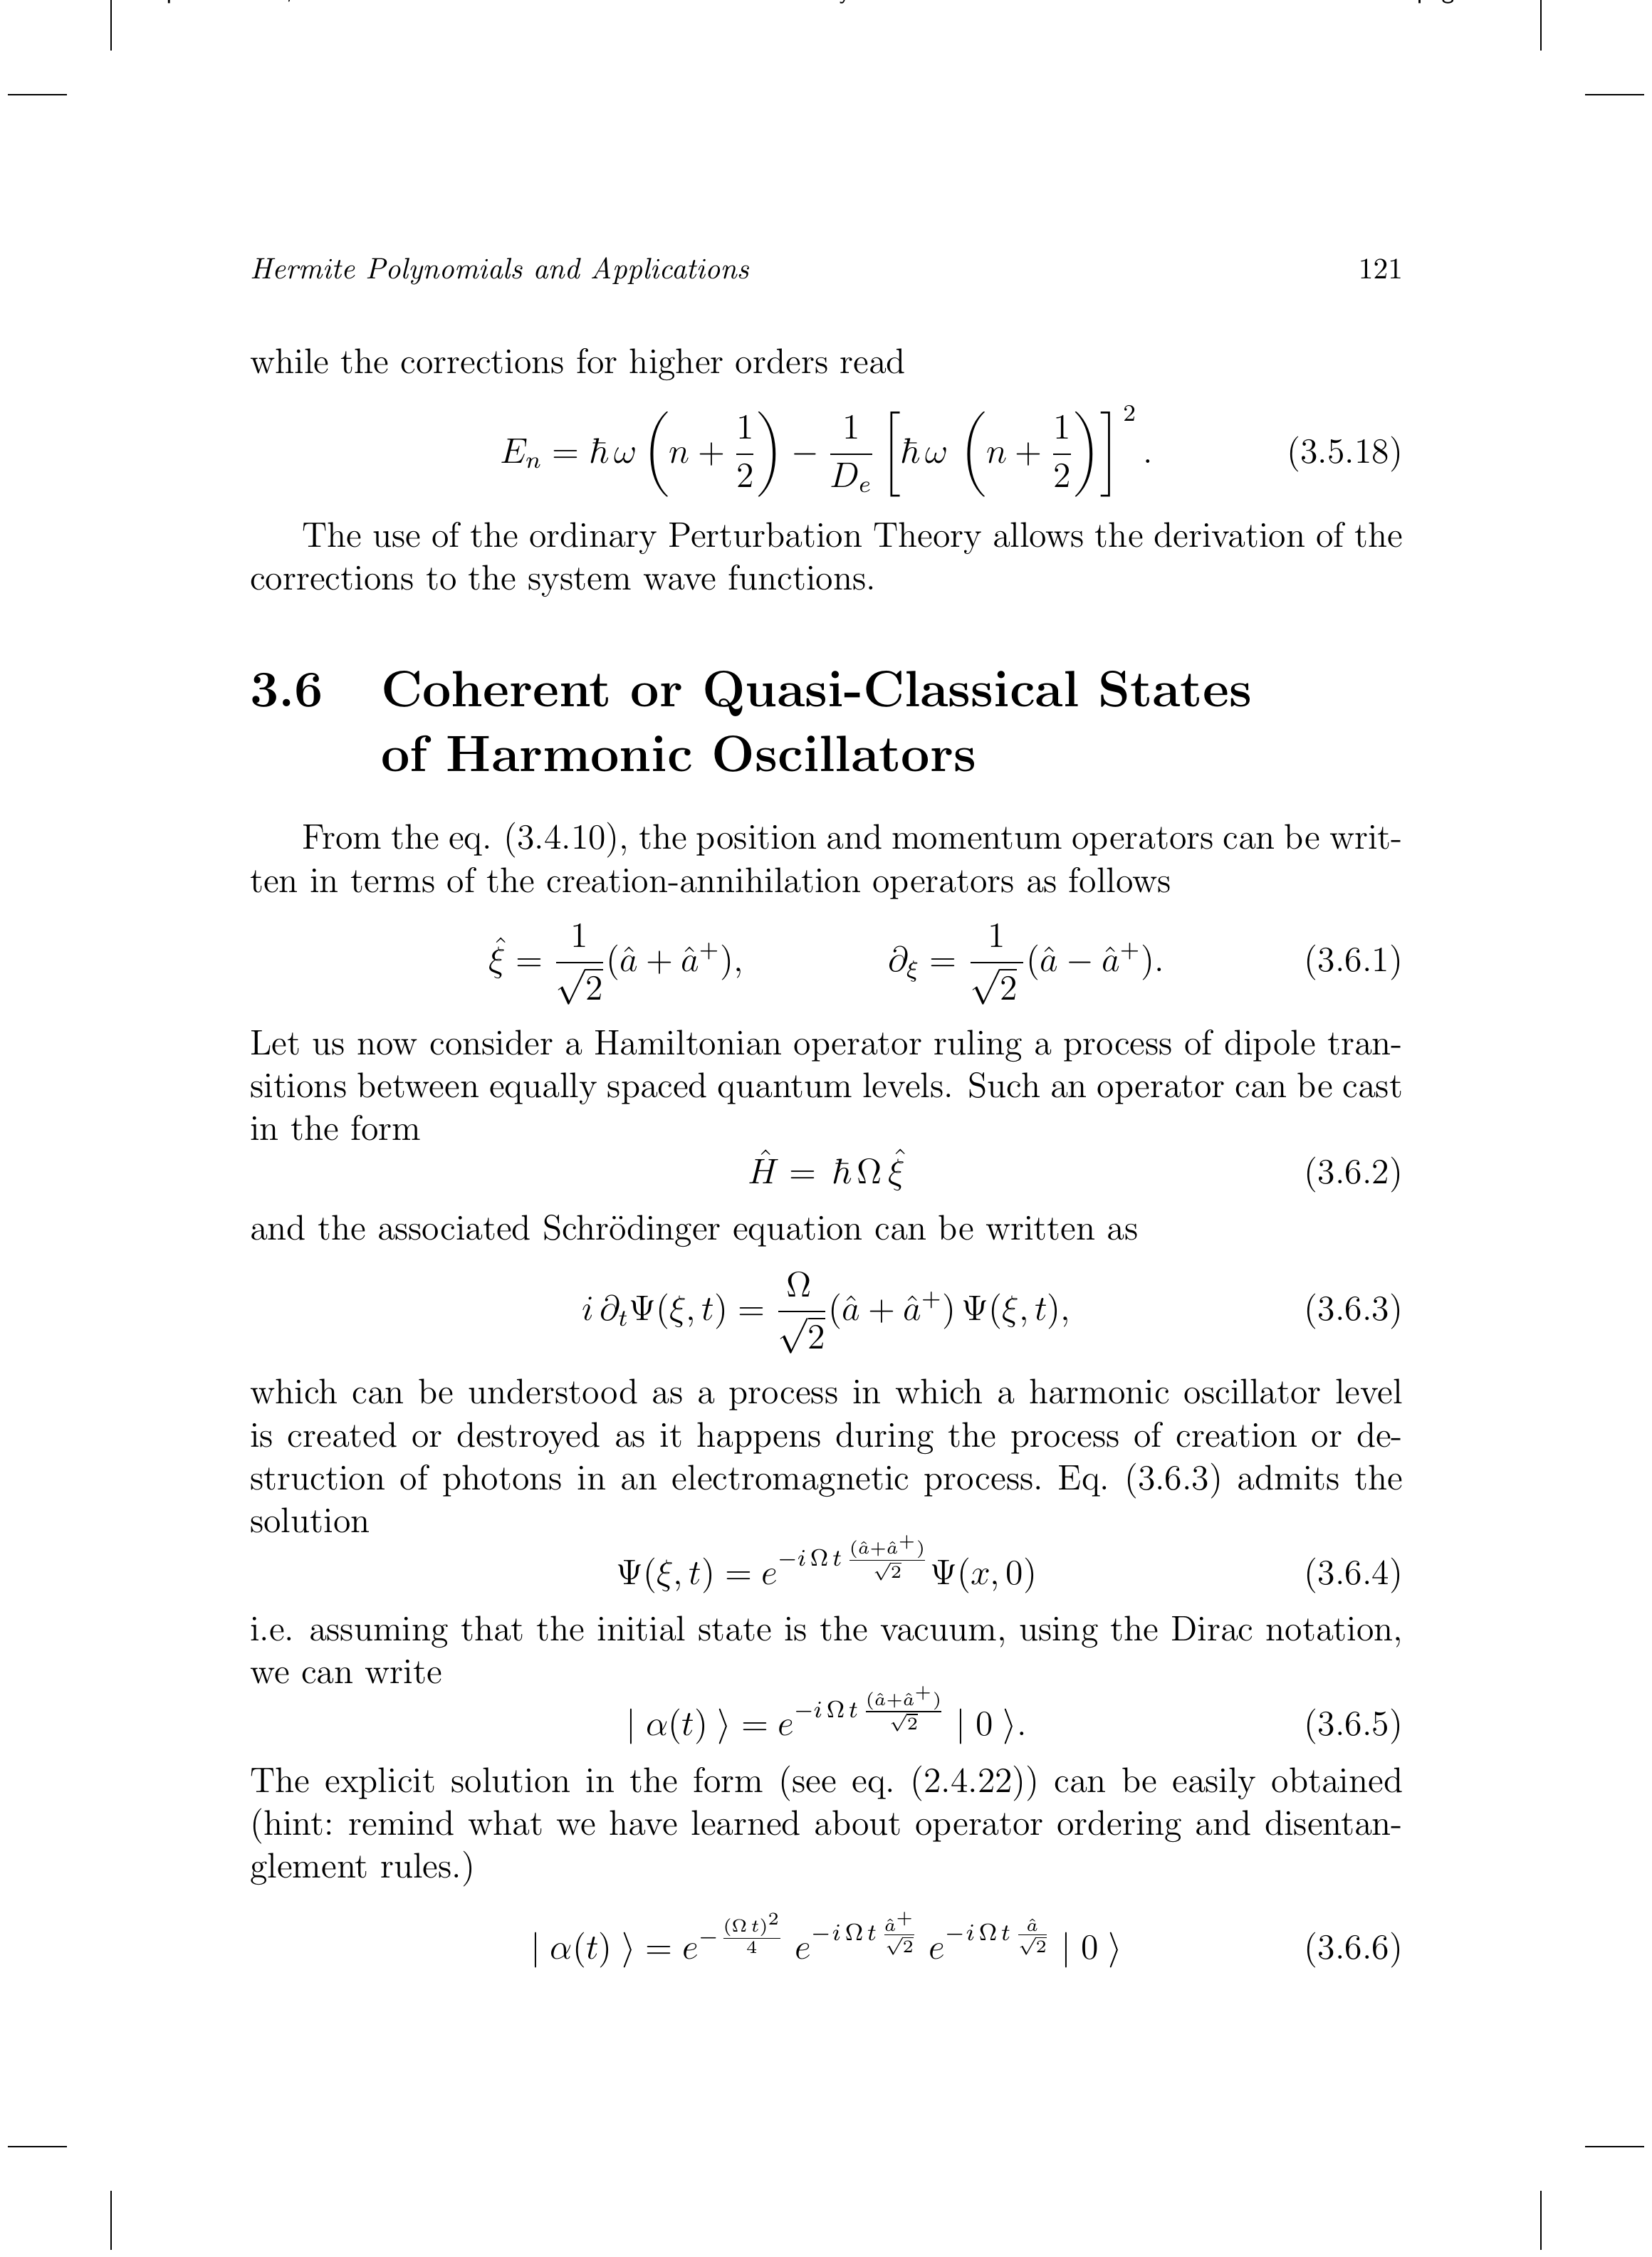
\includegraphics[max width=0.95\linewidth,keepaspectratio]{fig3_4.png}\caption{Morse 势（蓝色）与谐振子势（绿色）的比较。}
\label{fig:3.4}
\end{figure}

Morse 势的能级不像谐振子势那样等间距，其间隔随能量接近解离能而减小。

值得证明最低阶能级可由下式很好近似
\begin{equation}
E_n\approx\hbar\omega\!\left(n+\frac{1}{2}\right),\qquad
\nu\equiv a\sqrt{\frac{2D_e}{m}},
\label{eq:3.5.17}
\end{equation}
而更高阶的修正为
\begin{equation}
E_n\approx\hbar\omega\!\left(n+\frac{1}{2}\right)
-\frac{\hbar^2\omega^2}{4D_e}\!\left(n+\frac{1}{2}\right)^2.
\label{eq:3.5.18}
\end{equation}

利用普通微扰论可以推导系统波函数的修正。

% ------------------------------------------------------------------
\section{谐振子的相干态或准经典态}
\label{sec:3.6}

由式~\eqref{eq:3.4.10}，位置与动量算子可以用产生--湮灭算子表示为：
\begin{equation}
\hat\xi=\frac{1}{\sqrt{2}}\,(\hat a+\hat a^\dagger),\qquad
\hat p_\xi=\frac{i\hbar}{\sqrt{2}}\,(\hat a^\dagger-\hat a).
\label{eq:3.6.1}
\end{equation}

现在考虑一个支配等间距量子能级间偶极跃迁过程的哈密顿算子。这样的算子可以写成
\begin{equation}
\hat H=\hbar\Omega\,\hat\xi
\label{eq:3.6.2}
\end{equation}
相应的 Schr\"odinger 方程可以写成
\begin{equation}
i\partial_t\Psi(\xi,t)=\frac{\Omega}{\sqrt{2}}\,(\hat a+\hat a^\dagger)\,\Psi(\xi,t),
\label{eq:3.6.3}
\end{equation}
它可以理解为这样一个过程：谐振子能级被产生或消灭，如同电磁过程中光子产生或消灭一样。式~\eqref{eq:3.6.3} 有解
\begin{equation}
\Psi(\xi,t)=e^{-i\Omega t(\hat a+\hat a^\dagger)/\sqrt{2}}\,\Psi(x,0),
\label{eq:3.6.4}
\end{equation}
即假定初始态为真空态，用 Dirac 记号，我们可以写出
\begin{equation}
|\alpha(t)\rangle=
e^{-i\Omega t(\hat a+\hat a^\dagger)/\sqrt{2}}|0\rangle.
\label{eq:3.6.5}
\end{equation}
其闭式显式解（见式~\eqref{eq:2.4.22}）很容易获得
\noindent{\itshape （提示：回顾我们所学的算子排序与解缠规则。）}
\begin{equation}
|\alpha(t)\rangle=
e^{-(\Omega t)^2/4}\,
e^{-i\Omega t\hat a^\dagger/\sqrt{2}}\,
e^{-i\Omega t\hat a/\sqrt{2}}\,|0\rangle.
\label{eq:3.6.6}
\end{equation}
考虑到
\begin{equation}
e^{-i\Omega t\hat a/\sqrt{2}}\,|0\rangle=|0\rangle,
\label{eq:3.6.7}
\end{equation}
得到
\[
|\alpha(t)\rangle=
e^{-(\Omega t)^2/4}\,
\sum_{r=0}^{\infty}\frac{(-i\sqrt{2}\,\Omega t)^r}{2^{r/2}\,r!}\,
(\hat a^\dagger)^r|0\rangle
\]
\begin{equation}
=e^{-(\Omega t)^2/4}\,
\sum_{r=0}^{\infty}\frac{(-i\Omega t/\sqrt{2})^r}{r!}\,
|r\rangle.
\label{eq:3.6.8}
\end{equation}

``波函数'' $|\alpha(t)\rangle$ 由谐振子态的叠加给出，表示一个特定的量子态，称为\emph{相干态}，原因如下述。该态在给定时刻 $t$ 处于第 $m$ 个谐振子激发态的概率为
\begin{equation}
P_m(t)=|\langle m|\alpha(t)\rangle|^2
=e^{-(\Omega t)^2/2}\,\frac{(\Omega t/2)^{2m}}{m!}.
\label{eq:3.6.9}
\end{equation}
这个表达式是正交性质~\eqref{eq:3.4.18} 的推论，可识别为 Poisson 分布，找到量子谐振子激发态 $0,1,2,\ldots$ 的概率见图~\ref{fig:3.5}。

\begin{figure}[H]
\centering
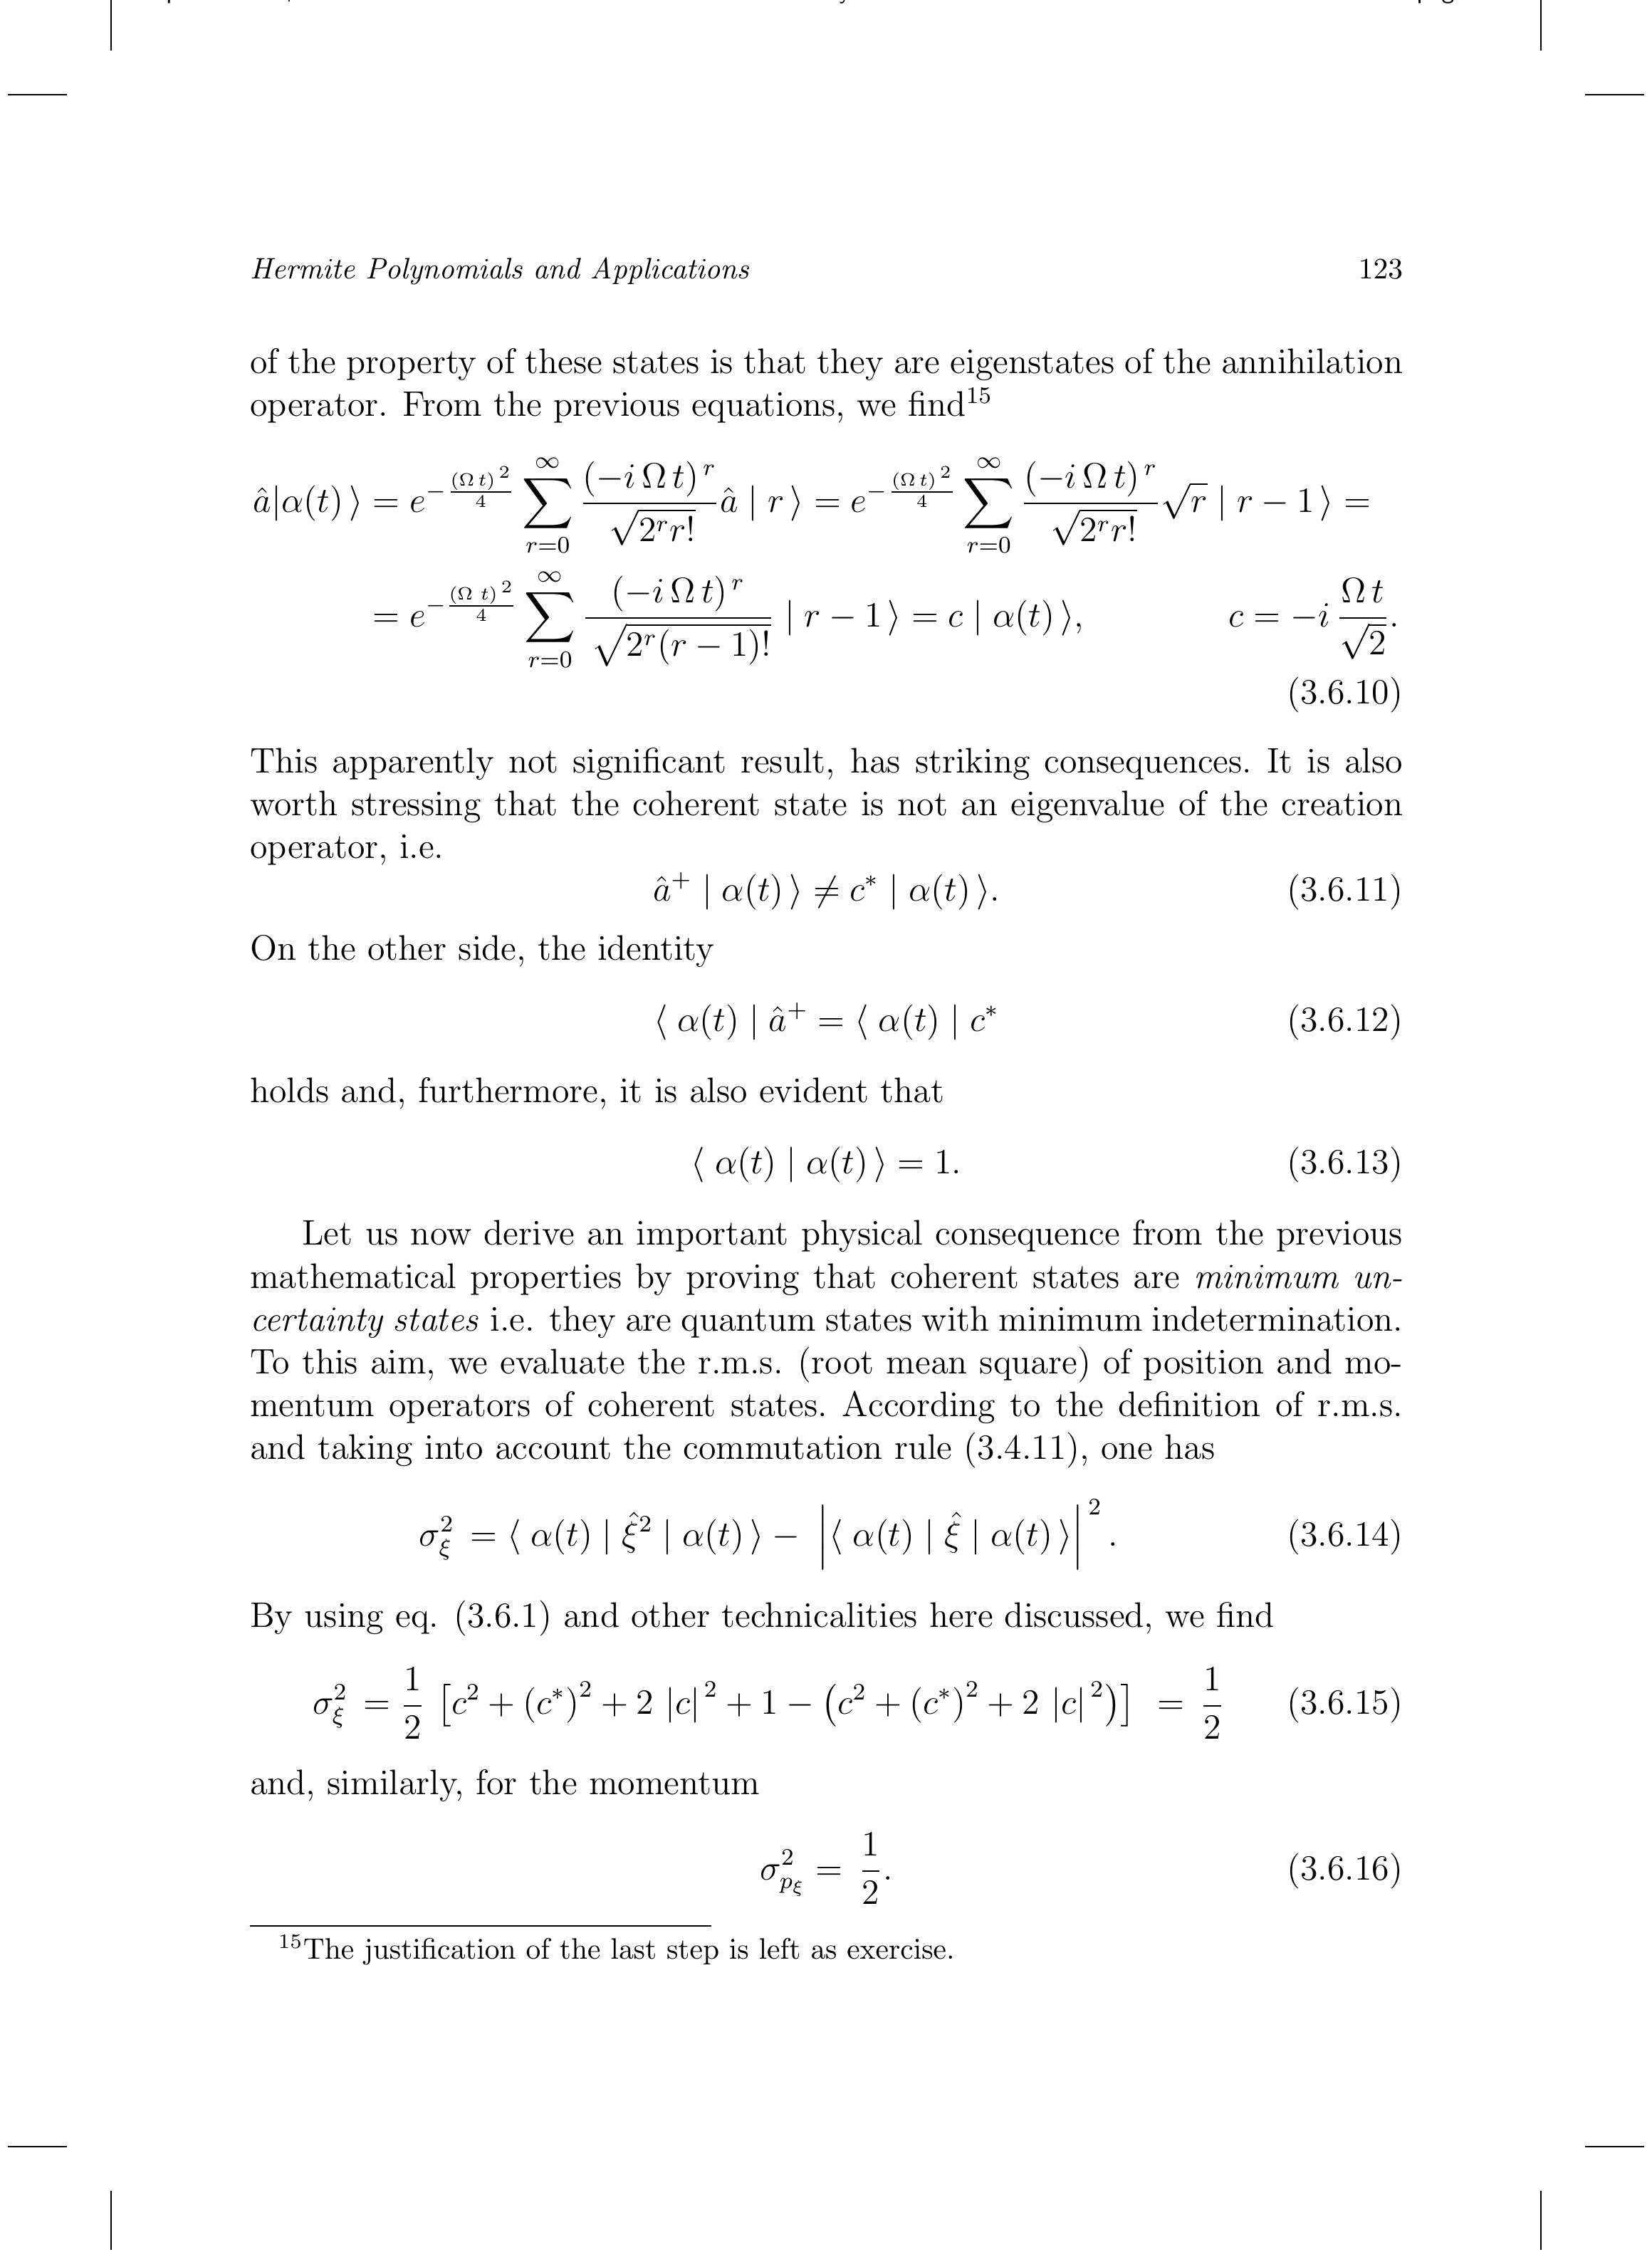
\includegraphics[max width=0.95\linewidth,keepaspectratio]{fig3_5.png}\caption{作为 $\Omega t$ 的函数，相干态处于 $|m\rangle$（$m=0,1,2,\ldots$）的概率。}
\label{fig:3.5}
\end{figure}

我们仅略谈相干态的性质，它们恰当地描述了激光型相干光源的电磁场。这些态的性质之一是它们是湮灭算子的本征态。由前面的方程，我们得到
\[
\hat a|\alpha(t)\rangle=
e^{-(\Omega t)^2/4}\,
\sum_{r=0}^{\infty}\frac{(-i\sqrt{2}\,\Omega t)^r}{2^{r/2}\,r!}\,
\hat a|r\rangle
=e^{-(\Omega t)^2/4}\,
\sum_{r=1}^{\infty}\frac{(-i\Omega t/\sqrt{2})^{r-1}}{(r-1)!}\,
|r-1\rangle
\]
\begin{equation}
=e^{-(\Omega t)^2/4}\,
\sum_{r=0}^{\infty}\frac{(-i\Omega t/\sqrt{2})^r}{r!}\,
|r\rangle
=c\,|\alpha(t)\rangle,\qquad
c=-\frac{i\Omega t}{\sqrt{2}}.
\label{eq:3.6.10}
\end{equation}
这个看似不重要的结果却具有惊人的推论。还值得强调，相干态不是产生算子的本征态，即
\begin{equation}
\hat a^\dagger|\alpha(t)\rangle\neq c^*|\alpha(t)\rangle.
\label{eq:3.6.11}
\end{equation}
另一方面，恒等式
\begin{equation}
\langle\alpha(t)|\hat a^\dagger=\langle\alpha(t)|c^*
\label{eq:3.6.12}
\end{equation}
成立，此外显然还有
\begin{equation}
\langle\alpha(t)|\alpha(t)\rangle=1.
\label{eq:3.6.13}
\end{equation}

现在我们从上述数学性质推导一个重要的物理推论，即证明相干态是\emph{最小不确定度态}，也就是不确定度最小的量子态。为此，我们计算相干态的位置与动量算子的均方根（r.m.s.）。根据 r.m.s. 的定义并考虑到对易规则~\eqref{eq:3.4.11}，有
\begin{equation}
\sigma_\xi^2=
\langle\alpha(t)|\hat\xi^2|\alpha(t)\rangle-
\bigl(\langle\alpha(t)|\hat\xi|\alpha(t)\rangle\bigr)^2.
\label{eq:3.6.14}
\end{equation}
利用式~\eqref{eq:3.6.1} 及此处讨论的其他技巧，我们得到
\begin{equation}
\sigma_\xi^2=\frac{1}{2}\bigl(c^2+(c^*)^2+2|c|^2+1\bigr)
-\frac{1}{2}\bigl(c^2+(c^*)^2+2|c|^2\bigr)=\frac{1}{2},
\label{eq:3.6.15}
\end{equation}
类似地，对动量
\begin{equation}
\sigma_p^2=\frac{\hbar^2}{2}.
\label{eq:3.6.16}
\end{equation}
回到有量纲的量，得到
\begin{equation}
\sigma_x^2=\frac{\hbar}{2m\omega},\qquad
\sigma_p^2=\frac{m\hbar\omega}{2},
\label{eq:3.6.17}
\end{equation}
因此
\begin{equation}
\sigma_x\,\sigma_p=\frac{\hbar}{2}.
\label{eq:3.6.18}
\end{equation}

另一方面，把同样的方法应用于 $n$ 态，可以证明不确定度随能级阶数增加：
\begin{equation}
(\sigma_x)_n^2=\frac{\hbar}{2m\omega}\,(2n+1),\qquad
(\sigma_p)_n^2=\frac{m\hbar\omega}{2}\,(2n+1),
\label{eq:3.6.19}
\end{equation}
\begin{equation}
(\sigma_x\,\sigma_p)_n=\frac{\hbar}{2}\,(2n+1).
\label{eq:3.6.20}
\end{equation}

这意味着，随着 $n$ 增大，波函数在位置和动量上都越来越展宽。相反，我们发现相干态具有最小不确定度态的独特性质。在量子态中，它们是最接近经典系统的态。

不过这一论断非常定性，需要进一步的说明。在图~\ref{fig:3.6} 中，我们给出了谐振子经典与量子概率的比较（详见注记 1）。

在低 $n$ 态的情形，量子与经典概率之间存在显著差异。在经典情形，谐振子大部分时间停留在远离平衡位置的地方，这意味着最大概率出现在位置较大的地方。相反，$n=0$ 时量子概率在 $x=0$ 附近取最大。我们还注意到有相当一部分空间在经典上是不被允许的。量子与经典概率随 $n$ 增大而趋于相似，这与对应原理完全一致。

现在可以解释为什么相干态更接近经典量子态\noindent{\itshape （提示：注意它是 $n$ 态的叠加……）}。

\begin{exercise}
重新考虑前面的结果，特别是它们的物理意义，并推导式~\eqref{eq:3.6.19}。
\end{exercise}

\begin{figure}[H]
\centering
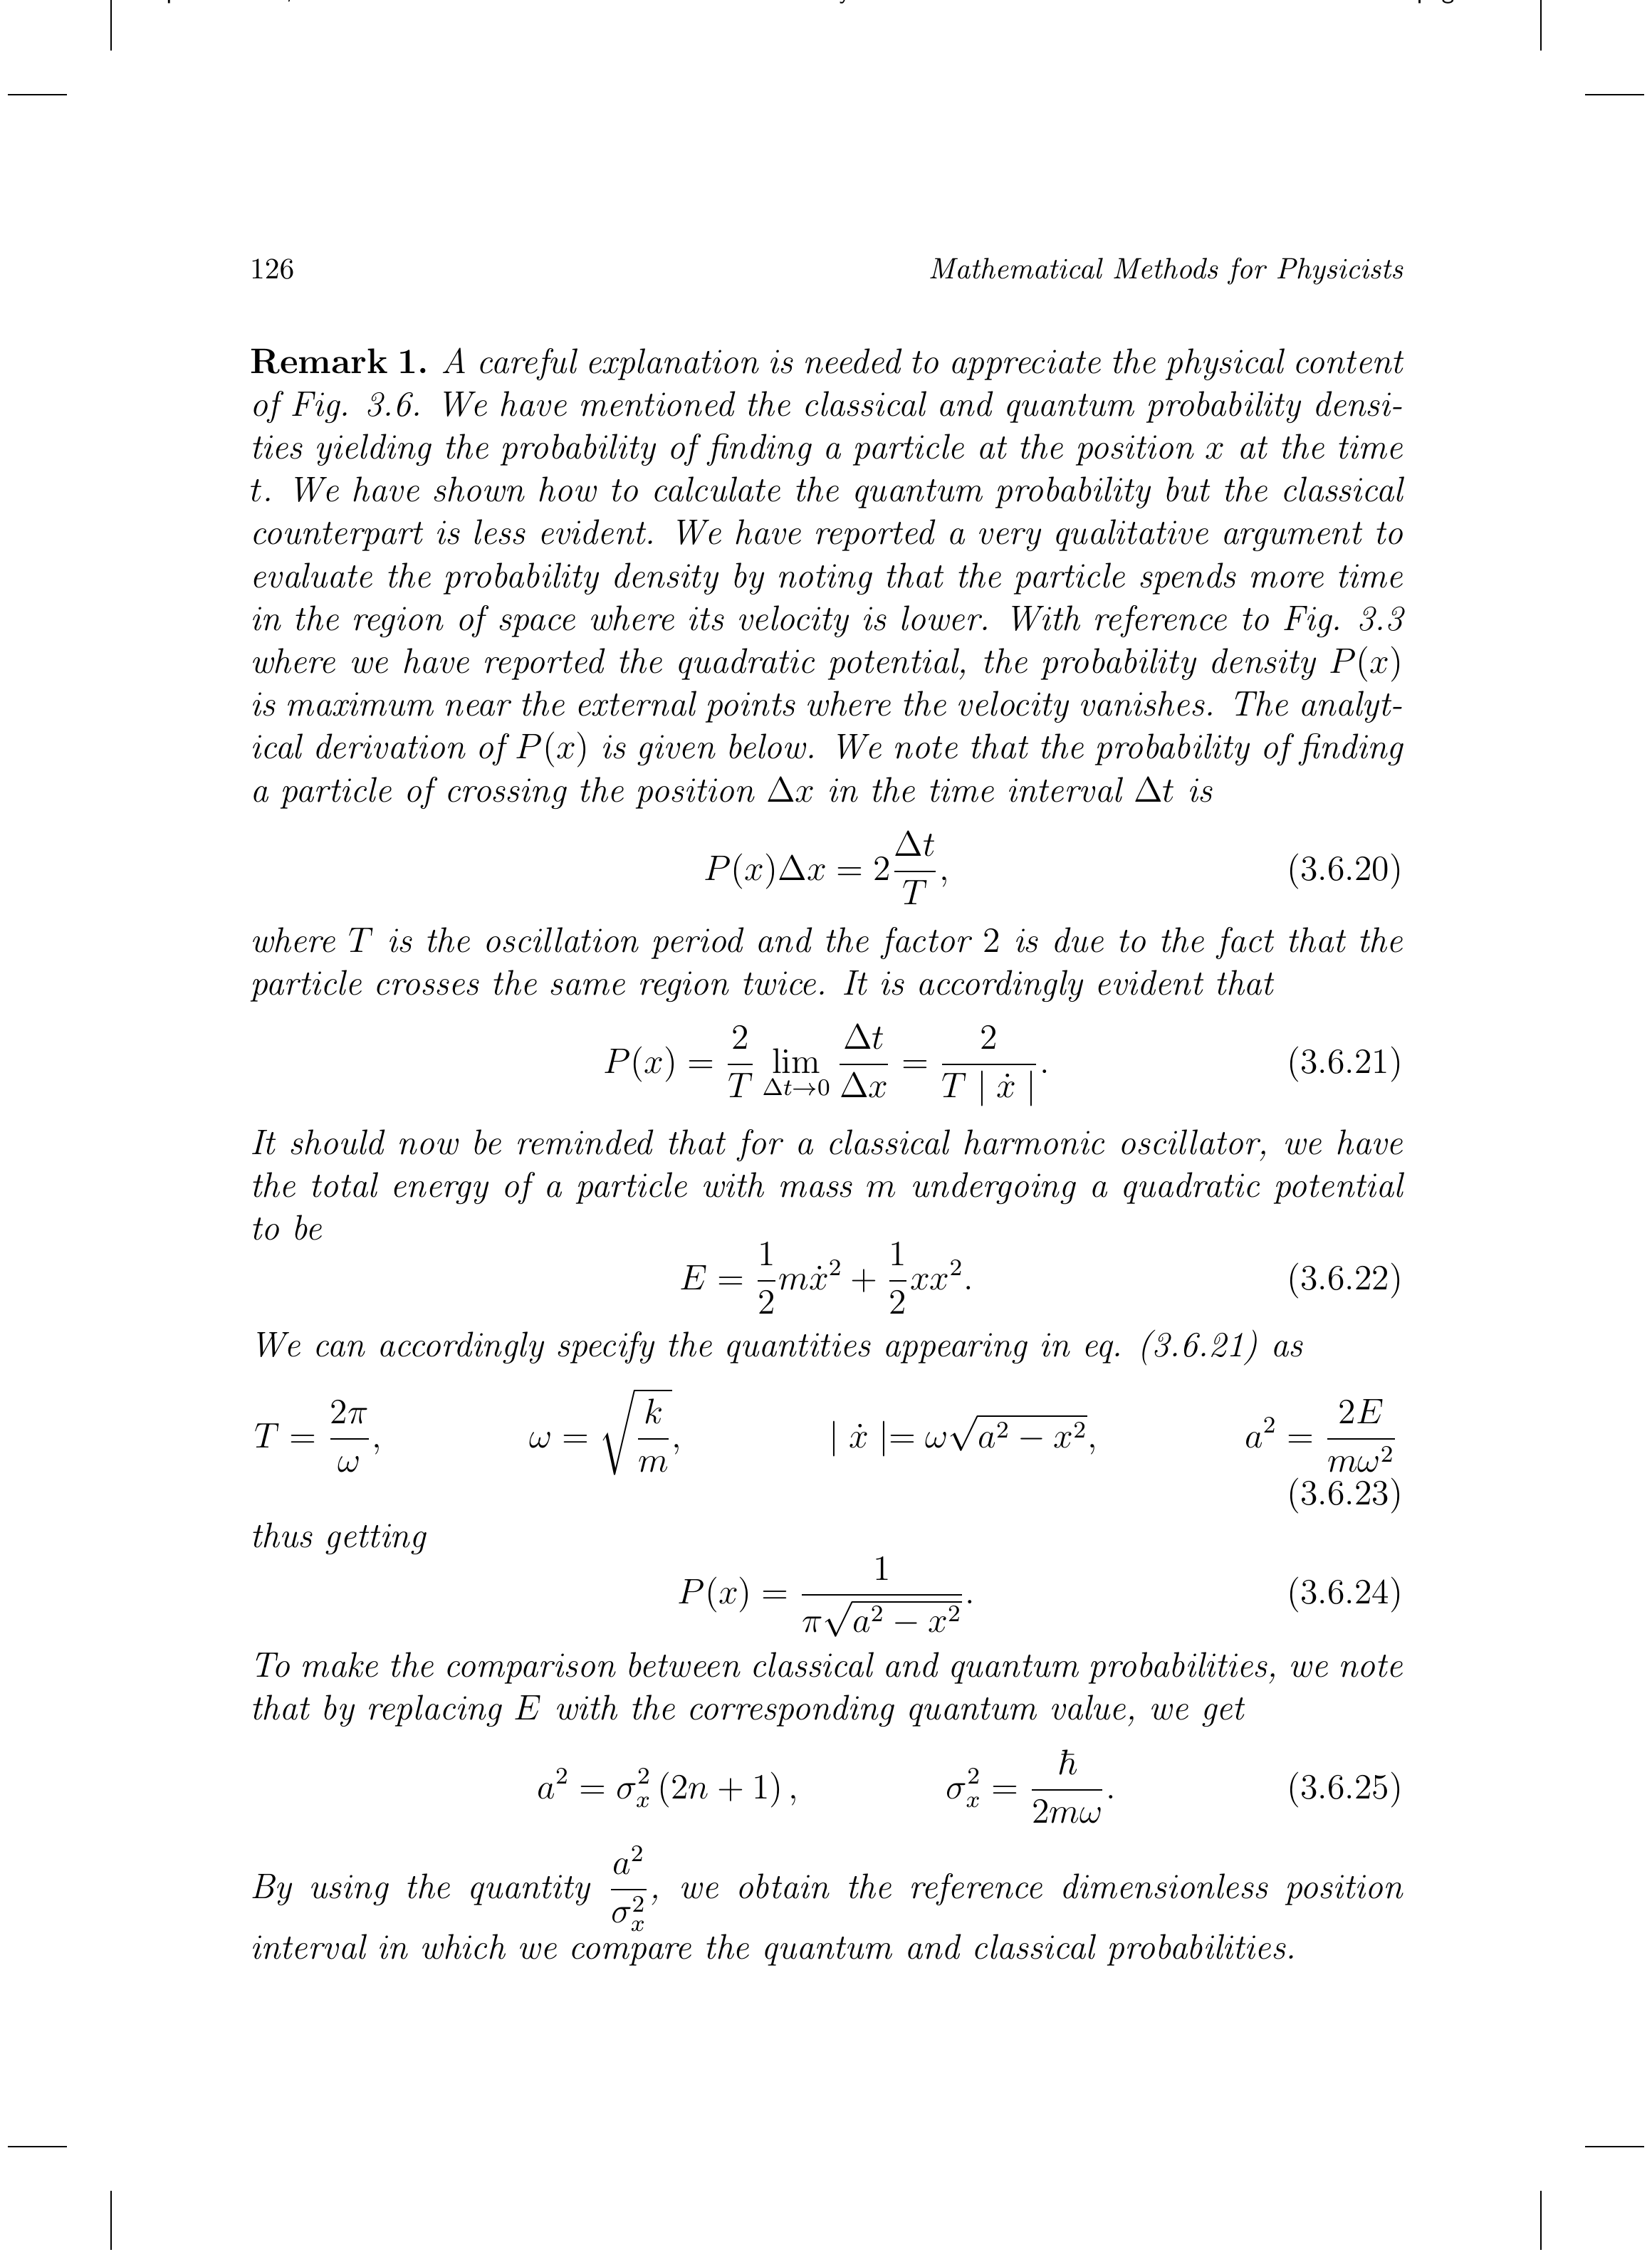
\includegraphics[max width=0.95\linewidth,keepaspectratio]{fig3_6.png}\caption{谐振子经典与量子概率的比较：(a)~$n=0$，(b)~$n=1$，(c)~$n=2$，(d)~$n=3$，(e)~$n=10$。}
\label{fig:3.6}
\end{figure}

\medskip
\noindent{\itshape 注记 1.} 需要仔细的说明才能领会图~\ref{fig:3.6} 的物理内容。我们提到了经典与量子概率密度，它们给出在时刻 $t$ 于位置 $x$ 处找到粒子的概率。我们已经说明如何计算量子概率，但经典对应物不那么明显。我们给出了一个非常定性的论证来估计概率密度：注意到粒子在速度较低的空间区域停留时间更长。参照图~\ref{fig:3.3} 中给出的二次势，概率密度 $P(x)$ 在速度为零的外侧点附近取最大。$P(x)$ 的解析推导如下。我们注意到，粒子在时间间隔 $\Delta t$ 内穿越位置 $\Delta x$ 的概率是
\begin{equation}
P(x)\,\Delta x=2\,\frac{\Delta t}{T},
\label{eq:3.6.23}
\end{equation}
其中 $T$ 是振荡周期，因子 2 来自粒子两次穿越同一区域。因此显然
\begin{equation}
P(x)=\lim_{\Delta t\to0}\frac{2\,\Delta t}{T\,\Delta x}
=\frac{2}{T\,|\dot x|}.
\label{eq:3.6.21}
\end{equation}
现在应提醒：对于经典谐振子，在二次势下运动的质量为 $m$ 的粒子的总能量为
\begin{equation}
E=\frac{1}{2}\,m\dot x^2+\frac{1}{2}\,k\,x^2.
\label{eq:3.6.22}
\end{equation}
因此可以把式~\eqref{eq:3.6.21} 中出现的量确定为
\[
T=\frac{2\pi}{\omega},\qquad \omega=\sqrt{\frac{k}{m}},\qquad
|\dot x|=\omega\sqrt{a^2-x^2},\qquad
a^2=\frac{2E}{m\omega^2},
\]
从而得到
\begin{equation}
P(x)=\frac{1}{\pi\sqrt{a^2-x^2}}.
\label{eq:3.6.24}
\end{equation}
为了进行经典与量子概率的比较，我们注意到把 $E$ 换成相应的量子值，得到
\[
a^2=\sigma_x^2\,(2n+1),\qquad \sigma_x^2=\frac{\hbar}{2m\omega}.
\]
利用量 $a^2$，我们获得比较量子与经典概率所用的无量纲位置参考区间。

% ------------------------------------------------------------------
\section{Jaynes--Cummings 模型}
\label{sec:3.7}

本节我们将引入涉及产生--湮灭算子与 Pauli 矩阵联合使用的问题。我们将研究 Jaynes--Cummings 模型（JC），它是已讨论的二能级原子模型（见第 1 章）的推广，其中经典电磁场保证上下能级之间的耦合。

如果我们不作经典场的假设，系统演化的分析应利用下列哈密顿量进行：
\begin{equation}
\hat H=\hat H_F+\hat H_I,\qquad
\hat H_F=\hbar\nu\,(\hat a^\dagger\hat a+\tfrac{1}{2}\hat\sigma_z),\qquad
\hat H_I=\hbar g\!\left(\hat a\,\hat\sigma_+\,e^{i\delta t}
+\hat a^\dagger\,\hat\sigma_-\,e^{-i\delta t}\right),
\label{eq:3.7.1}
\end{equation}
其中 $\nu$ 是电磁场的频率，$\omega$ 是两个能级之间的间隔。上述哈密顿量应作如下理解。
\begin{enumerate}
\item[(a)] 项 $\hat H_F$ 描述系统的自由能，包含两个贡献：第一个与电磁场相关（由 $\hbar\nu\hat a^\dagger\hat a$ 给出，与光子总数 $n_f$ 有关），第二个与二能级部分相关（由 $\frac{\hbar}{2}\omega\hat\sigma_z$ 给出）。我们强调算子 $\hat\sigma_z$ 与 $n_l$ 相关，即激发态与基态之间的布居差。
\end{enumerate}

\begin{figure}[H]
\centering
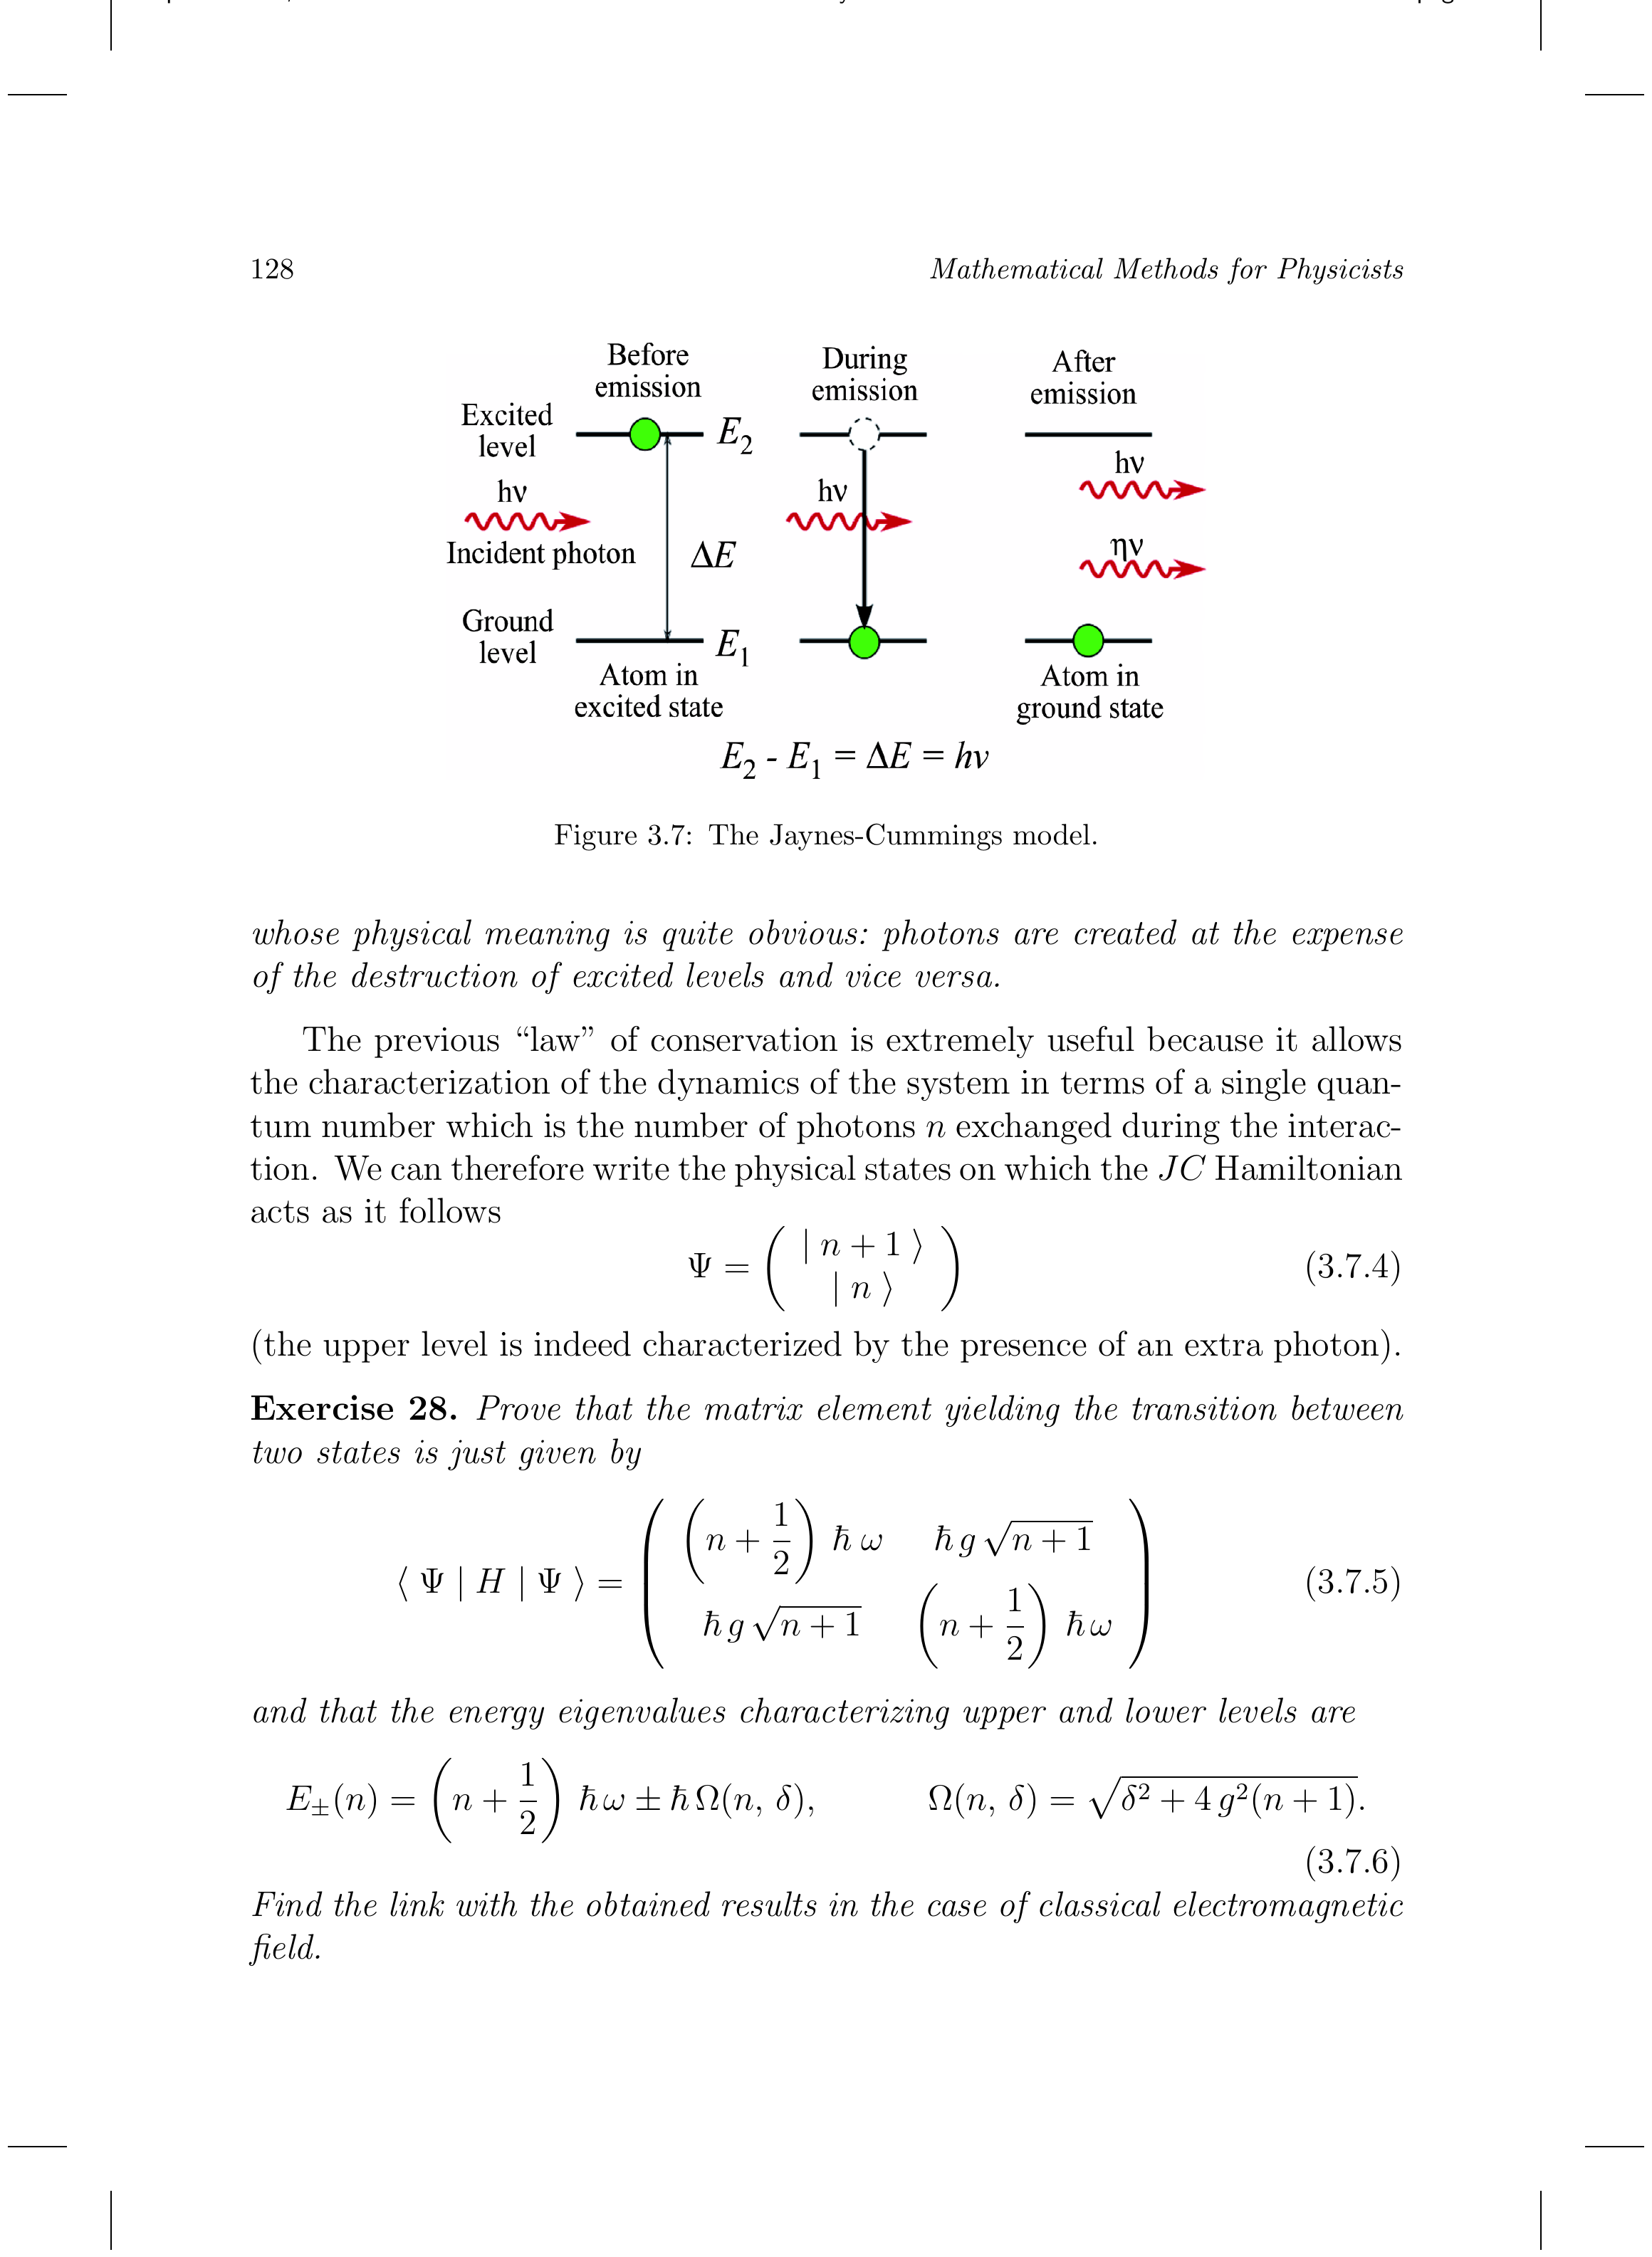
\includegraphics[max width=0.95\linewidth,keepaspectratio]{fig3_7.png}\caption{Jaynes--Cummings 模型：二能级原子与单个辐射模的耦合。}
\label{fig:3.7}
\end{figure}

\begin{exercise}
证明总哈密顿量与场部分对易，即
\begin{equation}
[\hat H,\hat H_F]=0,
\label{eq:3.7.2}
\end{equation}
并且这对应于下列守恒关系
\begin{equation}
n_f+n_l=k.
\label{eq:3.7.3}
\end{equation}
\end{exercise}

上述``守恒律''极其有用，因为它允许用一个量子数（即相互作用期间交换的光子数）来表征系统的动力学。因此我们可以写出 JC 哈密顿量作用的物理态如下
\begin{equation}
\Psi=\binom{|n+1\rangle}{|n\rangle},
\label{eq:3.7.4}
\end{equation}
（上能级确实以存在一个额外光子为特征）。

\begin{exercise}
证明给出两个态之间跃迁的矩阵元正是
\begin{equation}
\langle\Psi|\hat H|\Psi\rangle=
\begin{pmatrix}
\langle n|\hat H|n\rangle & \langle n|\hat H|n+1\rangle\\[4pt]
\langle n+1|\hat H|n\rangle & \langle n+1|\hat H|n+1\rangle
\end{pmatrix}
=
\frac{\hbar}{2}
\begin{pmatrix}
\omega & 2g\sqrt{n+1}\\
2g\sqrt{n+1} & -\omega
\end{pmatrix},
\label{eq:3.7.5}
\end{equation}
并且表征上下能级的能量本征值为
\begin{equation}
E_\pm(n)=\hbar\!\left(n+\frac{1}{2}\right)\nu
\pm\frac{\hbar}{2}\,\Omega(n,\delta),\qquad
\Omega(n,\delta)=\sqrt{\delta^2+4g^2(n+1)},
\label{eq:3.7.6}
\end{equation}
其中 $\delta=\omega-\nu$。找出与经典电磁场情形所得结果的联系。
\end{exercise}

% ------------------------------------------------------------------
\section{经典光学与 Hermite 多项式}
\label{sec:3.8}

在第 2 章中，我们以简单 Gaussian 光束的形式讨论了近轴形式的 Helmholtz 方程的解。这里我们将证明该方程的解与一种更复杂的形式相容，其中涉及 Hermite 多项式。这些解将被称为\emph{Hermite--Gauss} 光束。

为此，考虑热方程
\begin{equation}
\partial_t F(x,t)=\alpha\,\partial_x^2 F(x,t),\qquad
F(x,0)=H_n(\beta x)\,e^{-x^2/(2\sigma^2)}.
\label{eq:3.8.1}
\end{equation}
其解可以用 Weierstrass 变换求得：
\begin{equation}
F_n(x,t)=\frac{1}{\sqrt{4\pi\alpha t}}
\int_{-\infty}^{\infty}
e^{-\frac{(x-\xi)^2}{4\alpha t}}\,
H_n(\beta\xi)\,e^{-\xi^2/(2\sigma^2)}\,d\xi.
\label{eq:3.8.2}
\end{equation}

上述积分的计算使用生成函数方法，即
\[
I(x,t;\lambda)=\sum_{n=0}^{\infty}\frac{\lambda^n}{n!}\,F_n(x,t)
=\frac{1}{\sqrt{4\pi\alpha t}}
 \int_{-\infty}^{\infty}
 e^{-\frac{(x-\xi)^2}{4\alpha t}}\,
 e^{2\lambda\beta\xi-\lambda^2}\,
 e^{-\xi^2/(2\sigma^2)}\,d\xi.
\]

因此该问题可以用 Gauss 函数的积分规则轻松解决。我们得到
\[
F_n(x,t)=
\frac{\sigma^n}{\sqrt{\sigma^2(t)}}\,
H_n\!\left(\frac{x}{\sigma(t)},\frac{4\alpha\beta^2 t}{\sigma^4(t)}\right)\,
\exp\!\left[-\frac{x^2}{2\sigma^2(t)}\right],
\]
\begin{equation}
\sigma(t)=\sqrt{\sigma^2+4\alpha t},
\label{eq:3.8.4}
\end{equation}
考虑到式~\eqref{eq:3.3.9}，当 $\beta=\sigma^{-1}$ 时给出
\begin{equation}
F_n(x,t)=
\frac{1}{\sqrt{\sigma(t)}}\,
H_n\!\left(\frac{x}{\sigma(t)}\right)\,
\exp\!\left[-\frac{x^2}{2\sigma^2(t)}\right],
\label{eq:3.8.5}
\end{equation}
其中 $H_n$ 是规范 Hermite 多项式。

根据上述结果，我们可以把 Helmholtz 方程 (2.5.2) 的解写成
\begin{equation}
F_{l,m}(r,z)=
F_0\!\left(\frac{W}{W(z)}\right)\,
H_l\!\left(\frac{\sqrt{2}\,x}{W(z)}\right)\,
H_m\!\left(\frac{\sqrt{2}\,y}{W(z)}\right)\,
e^{-\frac{x^2+y^2}{W^2(z)}}\,
e^{-i\varphi-i\frac{k}{2R(z)}(x^2+y^2)+i\zeta(z)(l+m+1)},
\label{eq:3.8.6}
\end{equation}
它代表近轴近似的 Gauss--Hermite 光学模式（也称 $\mathrm{TEM}_{lm}$ 模）。在图~\ref{fig:3.8} 中，我们给出了前几个模式的横向分布的相应结构。还值得注意，这些模式的出现打破了 Gaussian 光束的柱对称性，因此不能在标量理论的框架内讨论。不过这一方面无法在本书中讨论。

\begin{figure}[H]
\centering
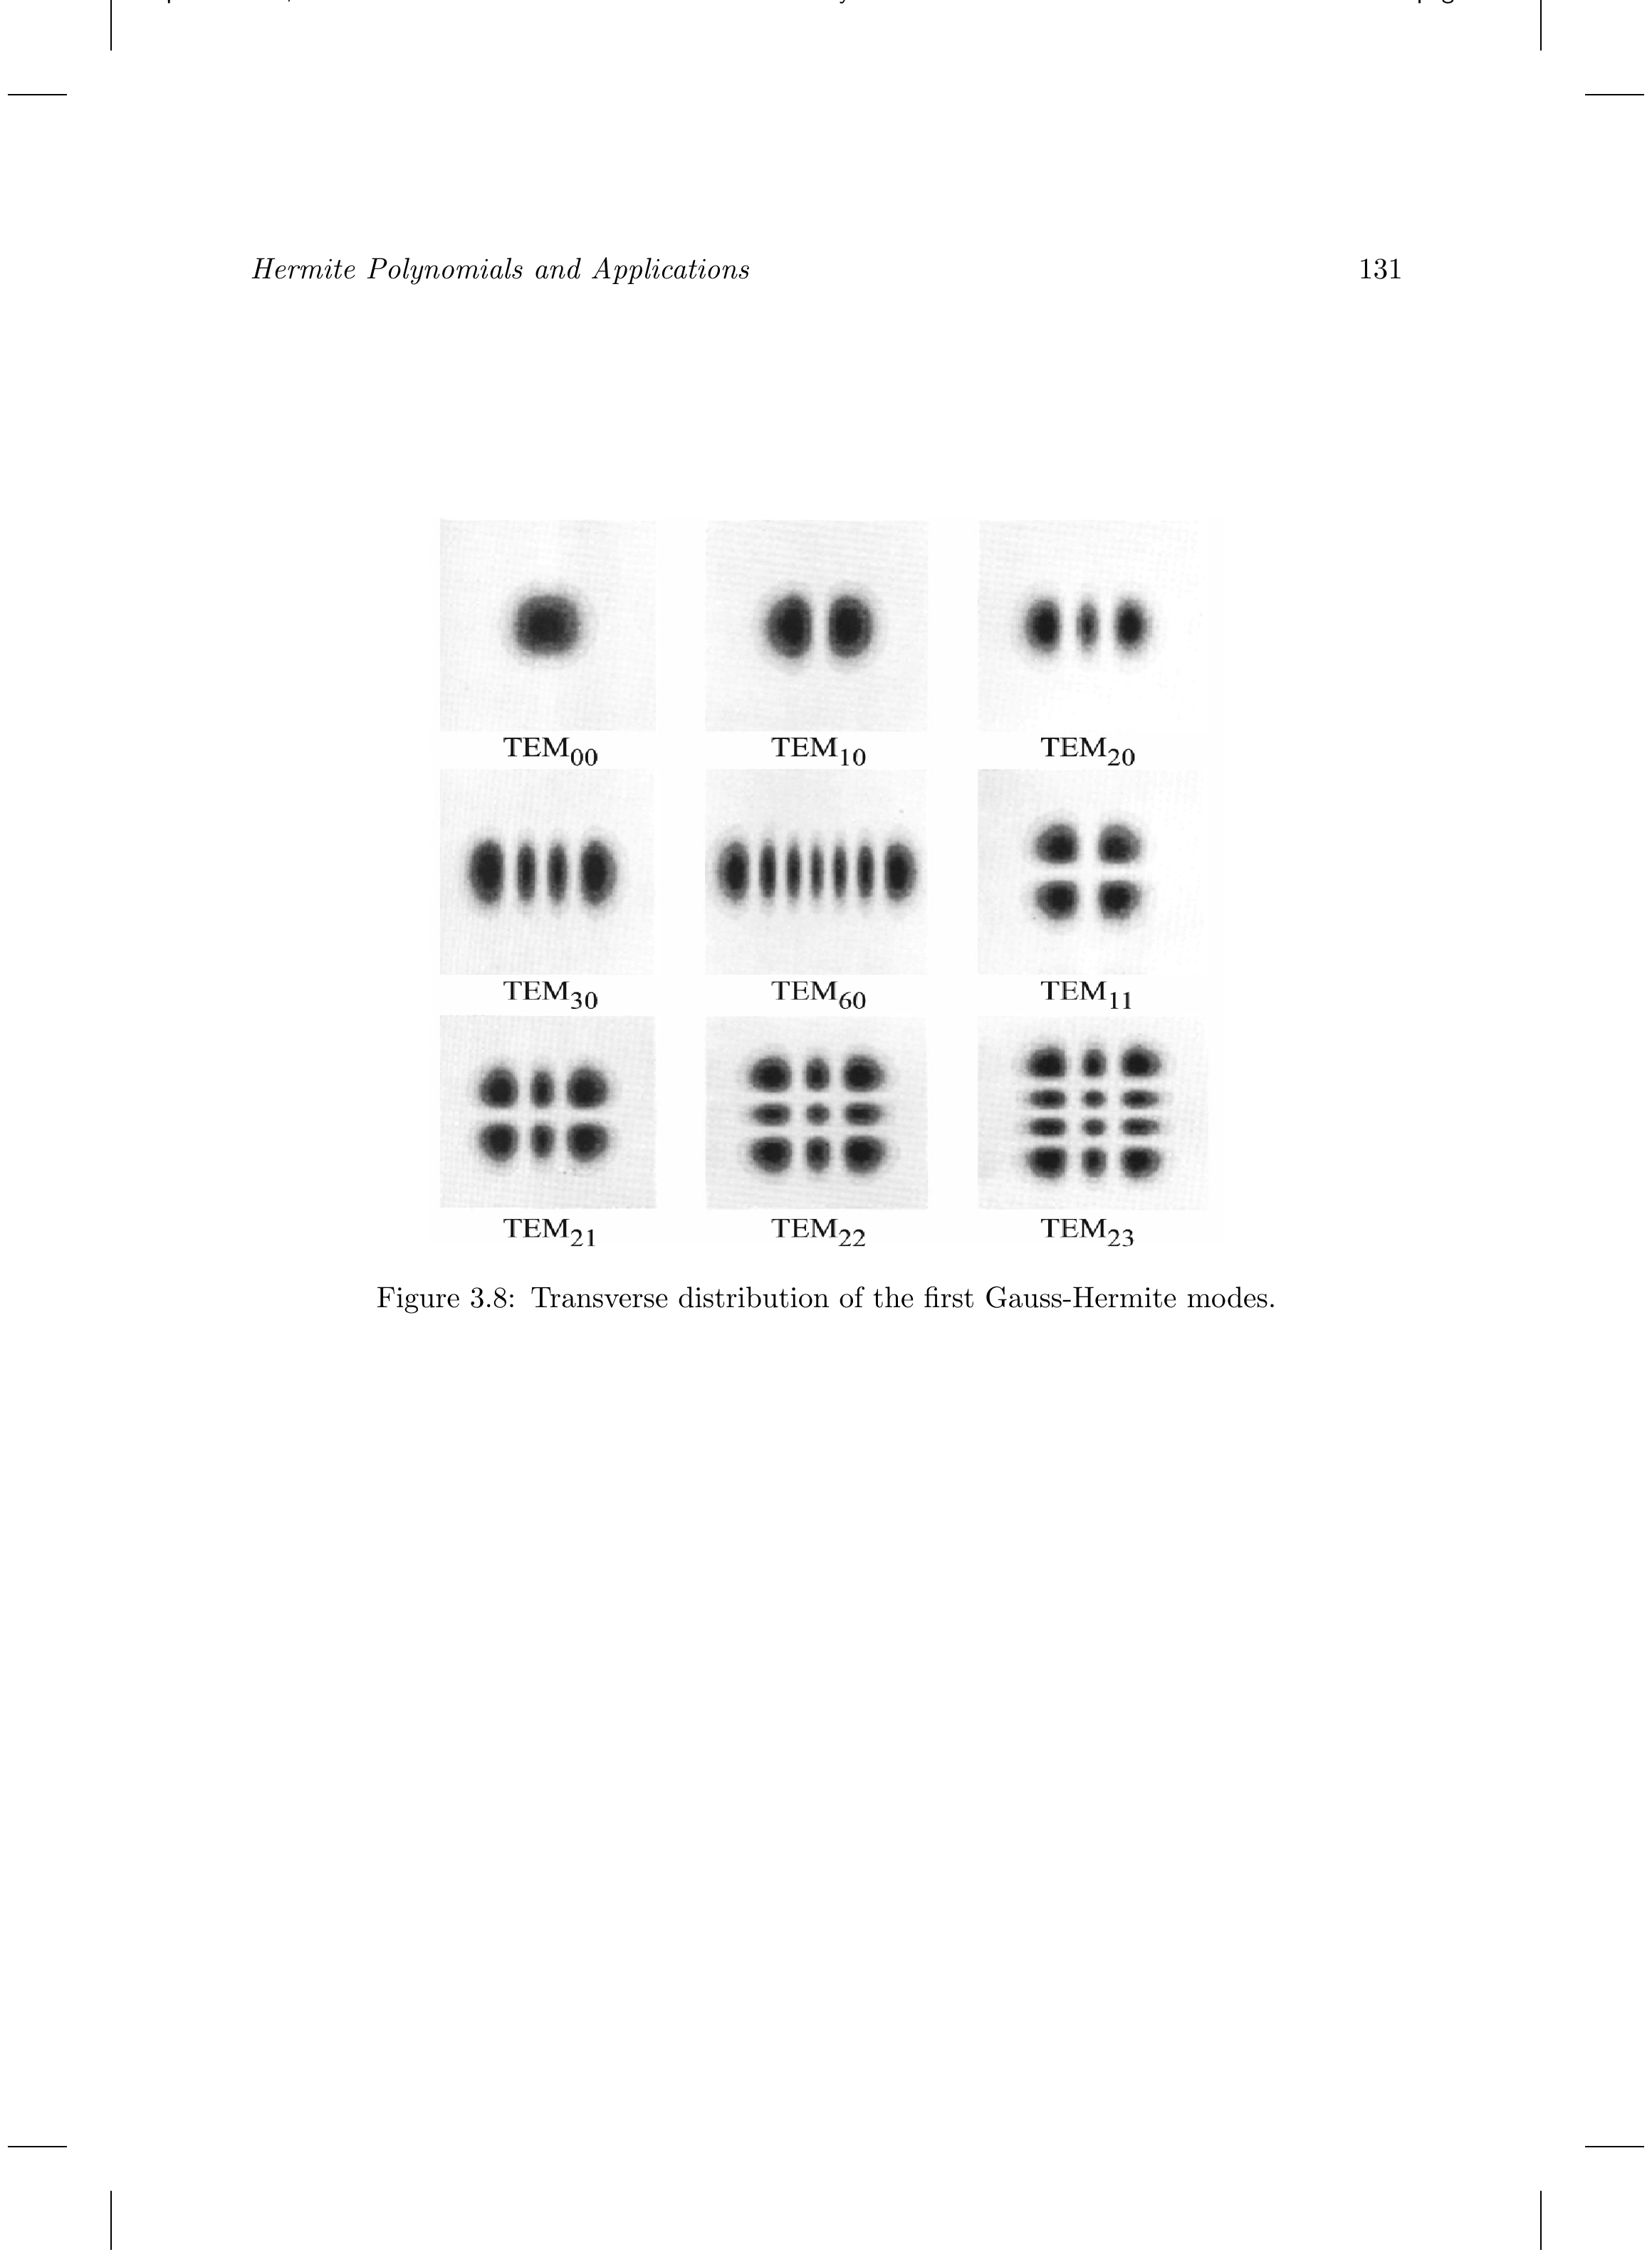
\includegraphics[max width=0.95\linewidth,keepaspectratio]{fig3_8.png}\caption{前几个 Gauss--Hermite $\mathrm{TEM}_{lm}$ 模的横向分布。}
\label{fig:3.8}
\end{figure}

在本章中，我们介绍了 Hermite 多项式的理论及其应用。我们采用了一种非常规的视角，其优点是提供了一个直接而灵活的形式体系。但我们邀请读者与下面参考文献中报告的常规（且更严格）处理进行比较。

% ------------------------------------------------------------------
\section*{参考文献}
\addcontentsline{toc}{section}{参考文献}

\subsection*{双变量 Hermite 多项式}
\begin{enumerate}[label={[\arabic*]}]
\item P.~App\'el, J.~Kamp\'e de F\'eriet,
      \emph{Fonctions Hypcrg\'eom\'etriques et Hypersph\'eriques,
      polyn\^omes d'Hermite}, Gautier-Villars, Paris, 1926.
\item Digital Library of Mathematical Functions,
      \emph{Orthogonal Polynomials, Classical Orthogonal
      Polynomials, Sums}, (18.18), National Institute of
      Standards and Technology, retrieved 30 January 2015.
\item H.W.~Gould, A.T.~Hopper,
      ``Operational formulas connected with two generalizations
      of Hermite polynomials'',
      \emph{Duke Math.\ J.} \textbf{29}, pp.~51--63, 1962.
\item N.N.~Lebedev, \emph{Special Functions and Their
      Applications}, Dover Books on Mathematics, 1972.
\item G.~Dattoli, ``Generalized polynomials, operational
      identities and their applications'',
      \emph{J.\ Comput.\ Appl.\ Math.} \textbf{118},
      pp.~111--123, 2000.
\item G.~Dattoli, S.~Lorezutta, A.~Torre,
      ``Miscellaneous identities of generalized Hermite
      polynomials'', \emph{Matematiche (Catania)} \textbf{52},
      pp.~337--343, 1997.
\item G.~Dattoli, S.~Lorezutta, G.~Maino, A.~Torre,
      ``Theory of multi-index multivariable Bessel functions
      and Hermite polynomials'',
      \emph{Matematiche (Catania)} \textbf{52},
      pp.~179--197, 1997.
\item G.~Dattoli, A.~Torre, M.~Carpanese,
      ``Operational rules and arbitrary order Hermite
      generating functions'',
      \emph{J.\ Math.\ Anal.\ Appl.} \textbf{227},
      pp.~98--111, 1998.
\item M.~Artioli, G.~Dattoli,
      ``The Geometry of Hermite Polynomials'',
      Wolfram Demonstrations Project, Mar.~2015,
      \url{http://demonstrations.wolfram.com/
      TheGeometryOfHermitePolynomials}.
\end{enumerate}

\subsection*{拟单项性（Monomiality）}
\begin{enumerate}[label={[\arabic*]},start=10]
\item G.~Dattoli, A.~Torre, G.~Mazzacurati,
      ``Quasi-monomials and isospectral problems'',
      \emph{Nuovo Cimento B} \textbf{112}, pp.~133--138, 1997.
\item G.~Dattoli, ``The Hermite and Laguerre Bessel Functions:
      A by Product of the Monomiality Principle'', in:
      D.~Cocolicchio, G.~Dattoli, H.M.~Srivastava (Eds.),
      \emph{Advanced Special Functions and Applications},
      Melfi, 1999, Aracne Editrice, Rome, p.~83, 2000.
\item P.~Blasiak, G.~Dattoli, A.~Horzela, K.~Penson,
      ``Representations of monomiality principle with
      Sheffer-type polynomials and boson normal ordering'',
      \emph{Phys.\ Lett.\ A} \textbf{352}, pp.~7--12, 2006.
\item J.F.~Steffensen, ``The poweroid, an extension of the
      mathematical notion of power'',
      \emph{Acta Math.} \textbf{73}, pp.~333--366, 1941.
\item A.V.~Turbiner, ``Quasi-exactly-solvable problems and
      $\mathfrak{sl}(2)$ algebra'',
      \emph{Commun.\ Math.\ Phys.} \textbf{118}, 46, 1988.
\end{enumerate}

\subsection*{Hermite 多项式作为正交集}
\begin{enumerate}[label={[\arabic*]},start=15]
\item D.T.~Haimo, C.~Markett, ``A representation theory for
      solutions of a higher-order heat equation I'',
      \emph{J.\ Math.\ Anal.\ Appl.} \textbf{168},
      pp.~89--107, 1992.
\item D.T.~Haimo, C.~Markett, ``A representation theory for
      solutions of a higher-order heat equation II'',
      \emph{J.\ Math.\ Anal.\ Appl.} \textbf{168},
      pp.~289--305, 1992.
\item G.~Dattoli, B.~Germano, P.E.~Ricci,
      ``Comments on monomiality, ordinary polynomials and
      associated bi-orthogonal functions'',
      \emph{Appl.\ Math.\ Comput.} \textbf{154},
      pp.~219--227, 2004.
\item G.~Dattoli, H.M.~Srivastava, K.~Zhukovsky,
      ``Orthogonality properties of the Hermite and related
      polynomials'',
      \emph{J.\ Comput.\ Appl.\ Math.} \textbf{182}(1),
      pp.~165--172, 2005.
\item G.~Dattoli, B.~Germano, P.E.~Ricci,
      ``Higher order Hermite polynomials, associated
      bi-orthogonal functions and generalized heat
      equations'',
      \emph{Integral Transforms Spec.\ Funct.} \textbf{16},
      2005.
\end{enumerate}

\subsection*{Hermite 多项式的几何}
\begin{enumerate}[label={[\arabic*]},start=20]
\item M.~Artioli, G.~Dattoli,
      ``The Geometry of Hermite Polynomials'',
      Wolfram Demonstrations Project, 2015,
      \url{http://demonstrations.wolfram.com/
      TheGeometryOfHermitePolynomials}.
\item M.~Artioli, G.~Dattoli,
      ``Geometric Properties of Generalized Hermite
      Polynomials'', Wolfram Demonstrations Project, 2015,
      \url{http://demonstrations.wolfram.com/
      GeometricPropertiesOfGeneralizedHermitePolynomials}.
\end{enumerate}

\subsection*{应用}
\begin{enumerate}[label={[\arabic*]},start=22]
\item W.H.~Louisell, \emph{Quantum Statistical Properties of
      Radiation}, Wiley, New York, 1973.
\item G.~Dattoli, P.L.~Ottaviani, A.~Torre, L.~Vazquez,
      ``Evolution operator equations, integration with
      algebraic and finite difference methods: applications
      to physical problems in classical and quantum
      mechanics'', \emph{Riv.\ Nuovo Cimento} \textbf{20},
      pp.~1--133, 1997.
\end{enumerate}

% ch4.tex — Laguerre 多项式、积分算子及其应用（中文版）

\chapter{Laguerre 多项式、积分算子及其应用}

\section{引言}

在本章中，我们将更深入地讨论特殊多项式及其在物理与数学问题中的相关应用。我们将处理 Laguerre 族并使用相应的双变量形式。正如在 Hermite 多项式的情形已经讨论过的，在经典多项式理论中引入额外变量特别有用。尽管可以通过简单的变换将其化为标准形式，但额外变量是发展基于算子形式体系的表述的关键工具。

本章基本上由两部分组成。在第一部分，我们将通过引入 Laguerre 多项式（LP）继续讨论``流行''的正交集。在第二部分，我们将用更一般的视角讨论特殊多项式理论，涉及 Appell 与 Sheffer 分类。不过我们将采用``非正统''的表述。

\section{Laguerre 多项式：定义与基本性质}

我们回到负导数算子（NDO）的定义，它满足
\begin{equation}
\hat D_x^{-n}\,1 = \frac{x^n}{n!}.
\label{eq:4.1.1}
\end{equation}

双变量 Laguerre 多项式定义为
\begin{equation}
L_n(x,y) = \bigl(y - \hat D_x^{-1}\bigr)^n 1.
\label{eq:4.1.2}
\end{equation}

利用普通二项式展开得到
\begin{equation}
L_n(x,y) = \sum_{r=0}^{n} \binom{n}{r} (-1)^r y^{\,n-r} \hat D_x^{-r}\,1
= \sum_{r=0}^{n} \frac{(-1)^r y^{\,n-r} x^r}{(n-r)!\,r!}.
\label{eq:4.1.3}
\end{equation}
当 $y=1$ 时，它化为普通 Laguerre 多项式 $L_n(x)$。

\begin{exercise}
证明伸缩恒等式
\begin{equation}
L_n(x,y) = y^n L_n\!\left(\frac{x}{y}\right).
\label{eq:4.1.4}
\end{equation}
\end{exercise}

\begin{figure}[h]
\centering
% 注：原书 Fig.4.1 为两组曲线图（y=1 与 y=-1/2），此处用文字占位
% 如有需要可补绘并替换为本地的 fig4_1a.pdf / fig4_1b.pdf
\setlength{\fboxsep}{6pt}\framebox[\textwidth]{\rule{0pt}{1.2cm}
  \textbf{图\,4.1（占位）：}前 5 个 Laguerre 多项式关于 $x$ 的图形，
  其中 (a) $y=1$，(b) $y=-\tfrac12$。}
\caption{前 5 个 Laguerre 多项式关于 $x$ 的图形：(a) $y=1$，(b) $y=-\tfrac12$。}
\label{fig:4.1}
\end{figure}

\paragraph{注记 1.} NDO 是积分算子：
$\hat D_x^{-1} f(x) = \int_a^x f(x')\,dx'$。
若我们不指明积分下限，则意味着 $a=0$。在第 9 章我们将对 NDO 形式体系作进一步说明。

\subsection*{拟单项性}

按照第 3 章引入的``拟单项性''定义，LP 是拟单项式。相应的乘法算子与求导算子为
\begin{equation}
\hat M = y - \hat D_x^{-1},
\qquad
\hat P = \hat{\mathcal L}\!\hat D_x = -\partial_x \hat D_x^{-1}.
\label{eq:4.1.7}
\end{equation}

因此 LP 可以用乘法算子定义为
\begin{equation}
L_n(x,y) = \hat M^n 1.
\label{eq:4.1.8}
\end{equation}

我们还可以推进该形式体系，采用下列定义
\begin{equation}
\hat{\mathcal L}\!\hat D_x
= -\partial_x \hat D_x^{-1},
\label{eq:4.1.9}
\end{equation}
其中 $\hat{\mathcal L}\!\hat D_x$ 有时称为\emph{Laguerre 导数}。其有效性可以通过注意下式验证：
\begin{equation}
\hat{\mathcal L}\!\hat D_x\,L_n(x,y)
= -\partial_x \hat D_x^{-1}(y-\hat D_x^{-1})^n 1
= n(y-\hat D_x^{-1})^{n-1}1
= n\,L_{n-1}(x,y).
\label{eq:4.1.10}
\end{equation}

由 $\hat M$ 与 $\hat P$ 的定义可以推出 $L_n(x,y)$ 满足的微分方程。注意到 $\hat D_x^{-1}\partial_x = \hat 1$，我们得到
\begin{equation}
\hat M\hat P\,L_n(x,y) = n\,L_n(x,y)
\label{eq:4.1.11}
\end{equation}
于是
\begin{equation}
y\,x\,L_n''(x,y) + (y-x)\,L_n'(x,y) = -n\,L_n(x,y).
\label{eq:4.1.12}
\end{equation}

Laguerre 导数有下列显著性质
\begin{equation}
\bigl(\hat{\mathcal L}\!\hat D_x\bigr)^n
= (-1)^n \partial_x^n x^n \partial_x^n,
\label{eq:4.1.13}
\end{equation}
可用归纳法证明。

\begin{exercise}
用上述性质证明反转恒等式
\begin{equation}
\frac{x^n}{n!}
= \sum_{s=0}^{n} \binom{n}{s} (-1)^s y^s L_{n-s}(x,y).
\label{eq:4.1.14}
\end{equation}
\emph{提示：}注意 $\frac{x^n}{n!} = (y - (y-\hat D_x^{-1}))^n 1$。
\end{exercise}

根据式~\eqref{eq:4.1.13}，把 Laguerre 导数反复作用于单项式 $q_n(x) = (-1)^n \frac{x^n}{n!}$ 得到
\begin{equation}
\bigl(\hat{\mathcal L}\!\hat D_x\bigr)^m q_n(x)
= \frac{n!}{(n-m)!}\,q_{n-m}(x), \qquad n>m.
\label{eq:4.1.15}
\end{equation}

\begin{exercise}
验证函数
\begin{equation}
C_0(x) = \sum_{l=0}^{\infty} \frac{q_l(x)}{l!}
\label{eq:4.1.16}
\end{equation}
是 Laguerre 导数的本征函数。
\end{exercise}

函数 \eqref{eq:4.1.16} 称为\emph{0 阶 Tricomi--Bessel 函数}；其行为见图~\ref{fig:4.2}。

\begin{figure}[h]
\centering
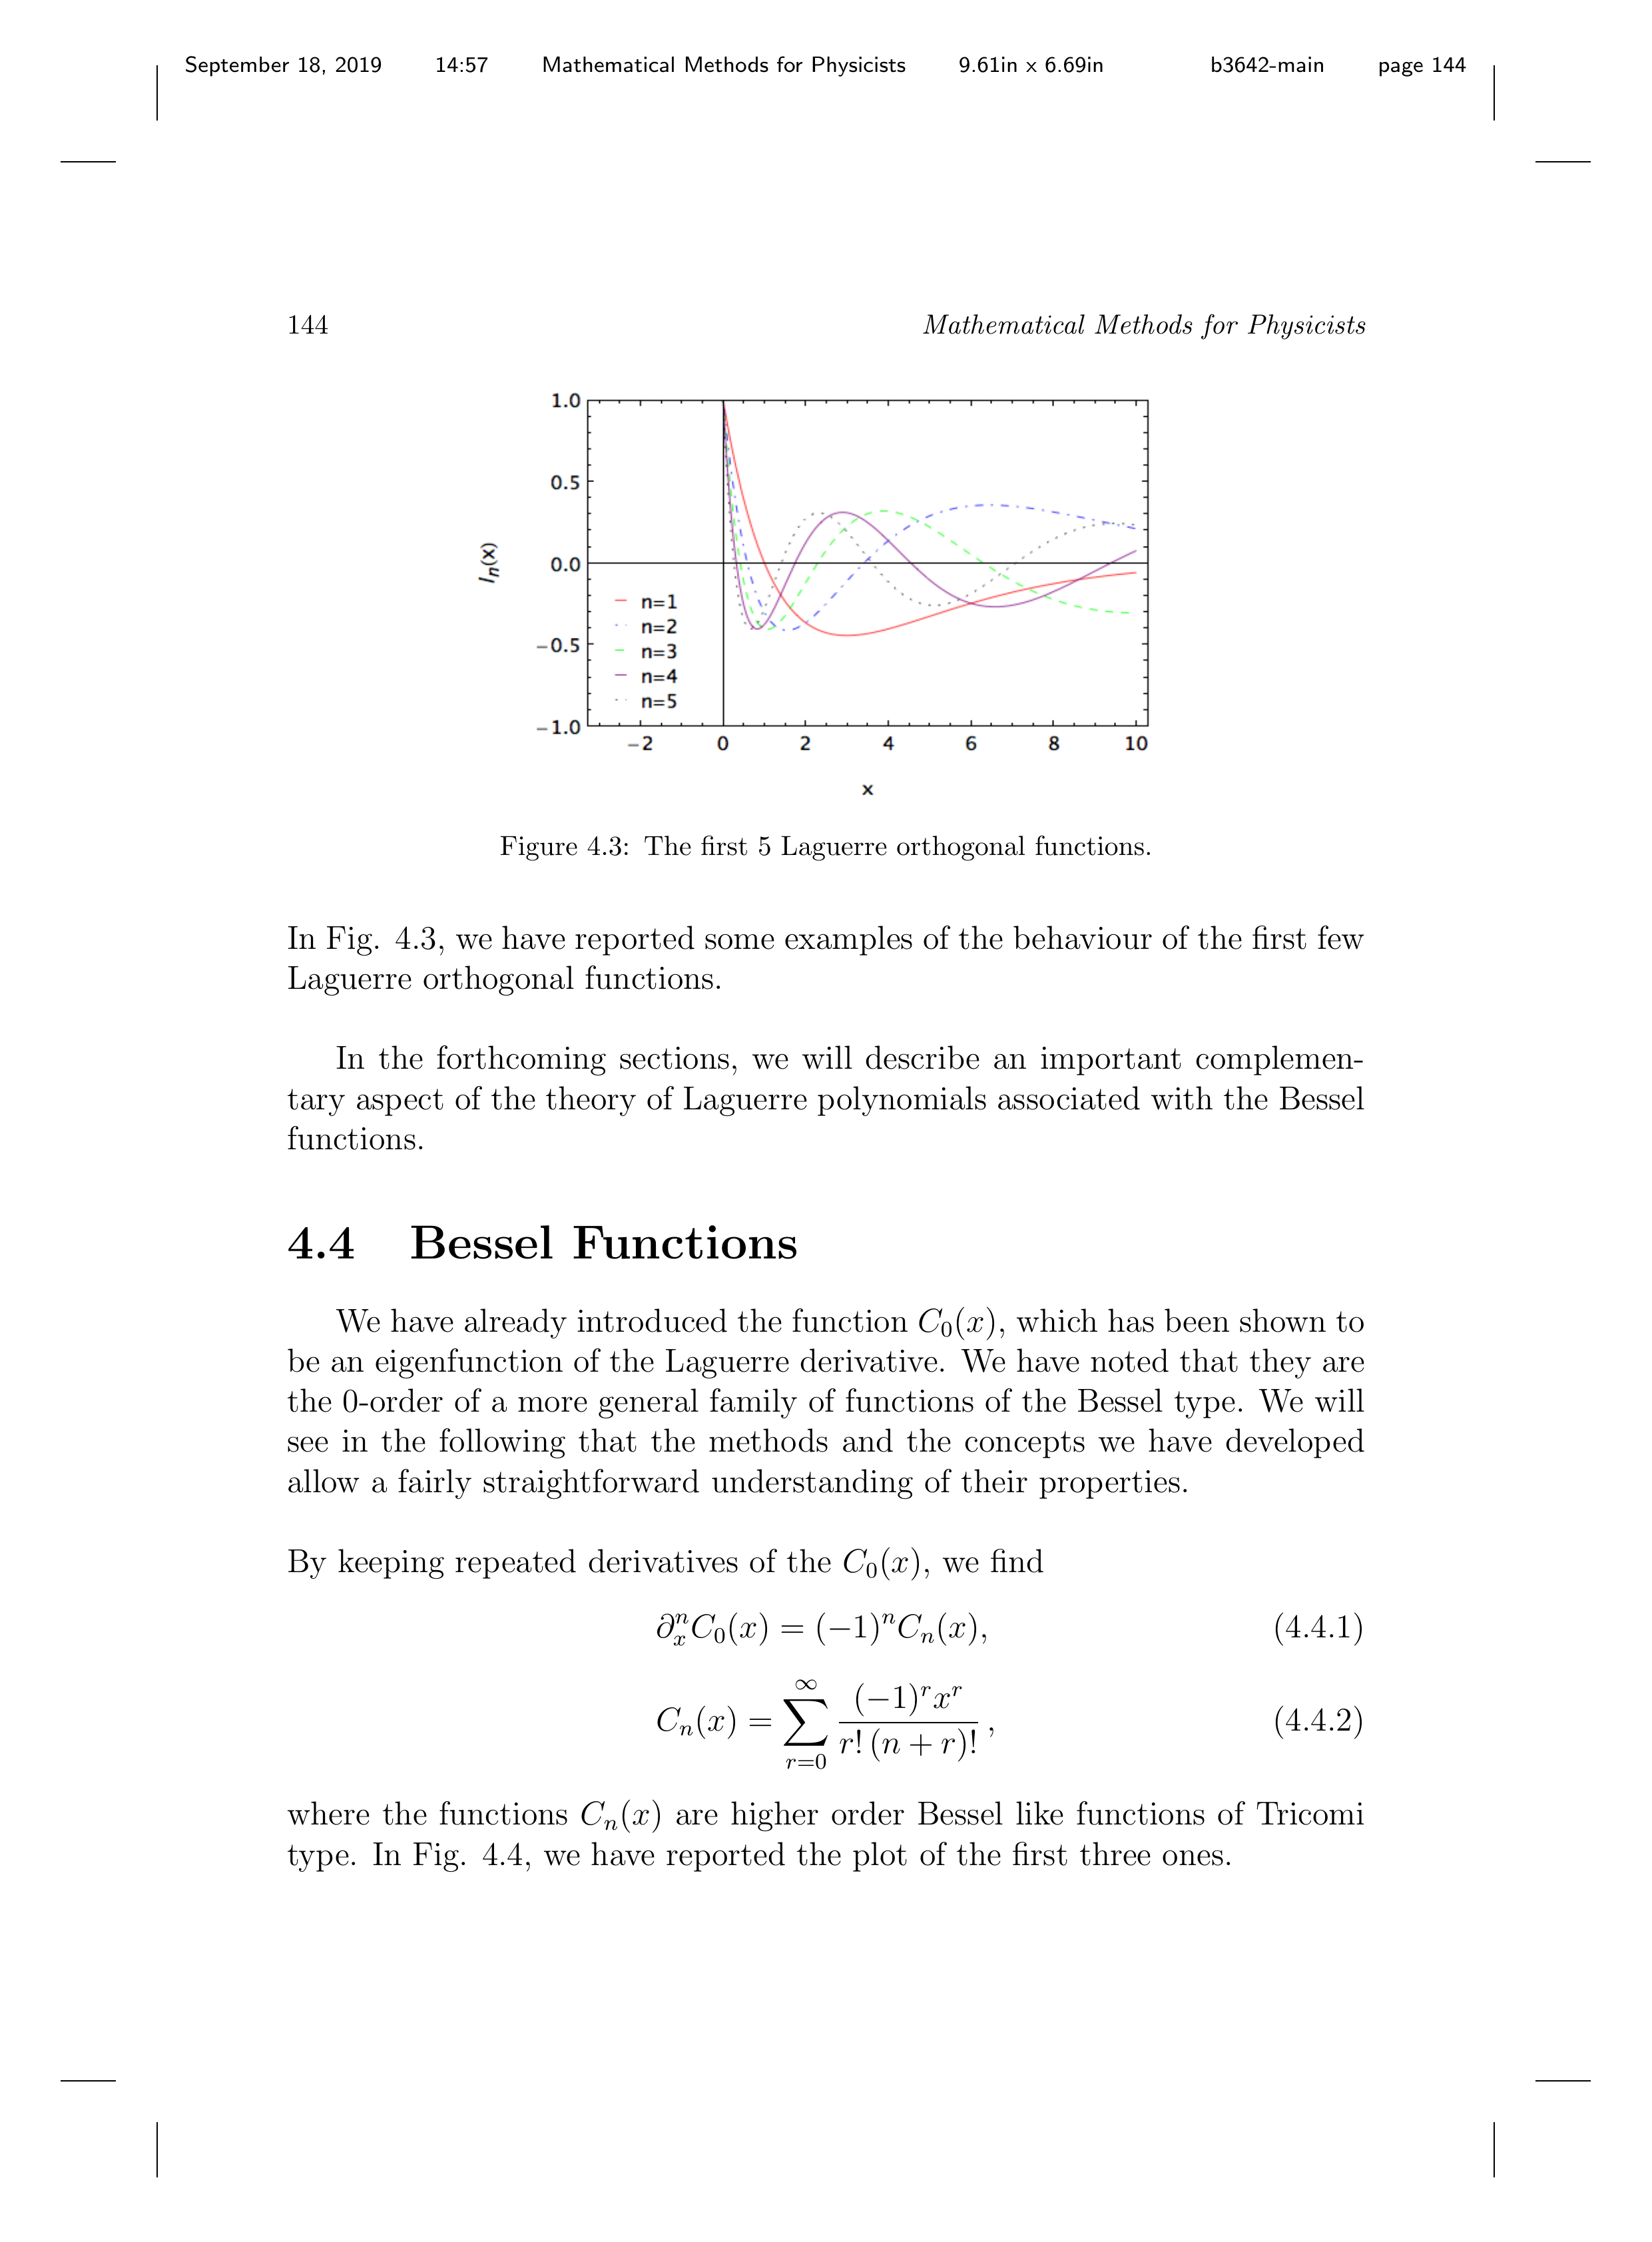
\includegraphics[max width=0.7\linewidth,keepaspectratio]{fig4_2.png}
\caption{0 阶 Tricomi--Bessel 函数 $C_0(x)$。}
\label{fig:4.2}
\end{figure}

在继续之前，应牢记下列对应关系：
\begin{equation}
\partial_x \;\longleftrightarrow\; \hat{\mathcal L}\!\hat D_x,
\qquad
x^n \;\longleftrightarrow\; q_n(x),
\qquad
e^x \;\longleftrightarrow\; C_0(x).
\label{eq:4.1.17}
\end{equation}

双变量 LP 满足偏微分方程
\begin{equation}
\begin{cases}
\partial_y L_n(x,y) = -\partial_x \hat D_x^{-1} L_n(x,y),\\[2pt]
L_n(x,0) = q_n(x),
\end{cases}
\label{eq:4.1.18}
\end{equation}
利用恒等式 \eqref{eq:4.1.10} 可以很容易陈述。这是 Hermite 多项式满足的热方程的类比。

由式~\eqref{eq:4.1.18}，我们还可以通过算子规则定义 LP
\begin{equation}
L_n(x,y) = e^{-y\,\partial_x \hat D_x^{-1}}
\!\left[(-1)^n\frac{x^n}{n!}\right].
\label{eq:4.1.20}
\end{equation}

\section{Laguerre 多项式的生成函数}

根据生成函数的定义，我们写出
\begin{equation}
G_L(x,y,t) = \sum_{n=0}^{\infty} \frac{t^n}{n!}
\bigl(y-\hat D_x^{-1}\bigr)^n 1
= e^{y t}\,e^{-t \hat D_x^{-1}} 1.
\label{eq:4.2.1}
\end{equation}

由于 $y$ 与 $\hat D_x^{-1}$ 对易，含逆导数算子的指数可以求和：
\begin{equation}
e^{-t \hat D_x^{-1}} 1
= \sum_{n=0}^{\infty} \frac{t^n}{n!}\,(-1)^n \hat D_x^{-n} 1
= \sum_{n=0}^{\infty} \frac{1}{n!}\,q_n(xt)
= C_0(xt).
\label{eq:4.2.2}
\end{equation}
于是
\begin{equation}
G_L(x,y,t) = e^{yt}\,C_0(xt).
\label{eq:4.2.3}
\end{equation}

还可以用乘法算子导出另一个生成函数：
\begin{equation}
S_L(x,y,t) = \sum_{n=0}^{\infty} t^n L_n(x,y)
= \frac{1}{1-yt}\,\exp\!\left(-\frac{xt}{1-yt}\right),
\qquad |yt|<1.
\label{eq:4.2.4}
\end{equation}

为证明此恒等式，由算子定义得到
\begin{align}
S_L(x,y,t)
&= \sum_{n=0}^{\infty} (\hat M t)^n 1
 = \frac{1}{1-\hat M t}\,1
 = \frac{1}{1-yt}\,\frac{1}{1+\dfrac{\hat D_x^{-1}t}{1-yt}} \notag\\
&= \frac{1}{1-yt}\,
\sum_{r=0}^{\infty} \left(-\frac{\hat D_x^{-1}t}{1-yt}\right)^{\!r} 1
 = \frac{1}{1-yt}\,\exp\!\left(-\frac{xt}{1-yt}\right).
\label{eq:4.2.5}
\end{align}

利用上述生成函数与式~\eqref{eq:4.1.20} 可以推导恒等式
\begin{equation}
e^{-y\,\partial_x \hat D_x^{-1}} e^{-xt}
= \frac{1}{1-yt}\,\exp\!\left(-\frac{xt}{1-yt}\right),
\label{eq:4.2.6}
\end{equation}
这是涉及 Laguerre 导数指数算子的 Glaisher 恒等式（见式~\eqref{eq:2.2.18}）的类比。

另一方面，式~\eqref{eq:4.2.5} 中的生成函数 $S_L$ 允许我们为双变量 LP 建立下列积分表示：
\begin{equation}
L_n(x,y) = \frac{e^{x/y}}{n!}\int_0^{\infty} e^{-s}\left(\frac{ys}{}\right)^{\!n}
C_0\!\left(\frac{xs}{y}\right) ds,
\label{eq:4.2.7}
\end{equation}
其有效性可以用生成函数 \eqref{eq:4.2.4} 验证。

\section{Laguerre 多项式的正交性质}

根据式~\eqref{eq:4.1.20}，Laguerre 多项式由与 Hermite 多项式类似的算子定义确定。下列恒等式是同一定义的副产品：
\begin{equation}
L_n(x,y+z) = e^{-z\,\partial_x \hat D_x^{-1}} L_n(x,y).
\label{eq:4.3.1}
\end{equation}

现在我们可以证明 LP 构成一个正交集。我们从方程
\begin{equation}
\begin{cases}
\partial_y F(x,y) = -\partial_x \hat D_x^{-1} F(x,y),\\[2pt]
F(x,0) = g(x),
\end{cases}
\label{eq:4.3.2}
\end{equation}
的解出发，它在 Hermite 多项式情形中起热方程的作用。其解可以写成积分形式
\begin{equation}
F(x,y) = \frac{e^{x/y}}{y}\int_0^{\infty} e^{-\sigma}\,
C_0\!\left(\frac{x\sigma}{y}\right) g(-y\sigma)\,d\sigma.
\label{eq:4.3.3}
\end{equation}

若 $g(x) = \sum_{n=0}^{\infty} a_n \frac{x^n}{n!}$，我们可以写出
\begin{equation}
F(x,y) = e^{-y\,\partial_x \hat D_x^{-1}}
\sum_{n=0}^{\infty} a_n \frac{x^n}{n!}
= \sum_{n=0}^{\infty} a_n (-1)^n L_n(x,y).
\label{eq:4.3.4}
\end{equation}

利用恒等式 \eqref{eq:4.2.7} 可以把上述方程改写为
\begin{equation}
F(x,y) = \sum_{n=0}^{\infty} (-1)^n a_n L_n(x,y)
= \frac{e^{x/y}}{y}\int_0^{\infty} e^{-\sigma}\,
C_0\!\left(\frac{x\sigma}{y}\right) g(-y\sigma)\,d\sigma,
\label{eq:4.3.5}
\end{equation}
前提是可以交换求和与积分的次序。

因此我们可以像上一节那样进行，得到与 Laguerre 族双正交的函数集。为简单起见，取 $y=1$，并假定 $g(x)$ 可以按 LP 展开为级数：
\begin{equation}
g(x) = \sum_{n=0}^{\infty} \alpha_n L_n(x).
\label{eq:4.3.6}
\end{equation}

把 $\partial_x \hat D_x^{-1}$ 作用于该展开式得到
\begin{equation}
\partial_x \hat D_x^{-1} \Phi(x)
= \sum_{n=0}^{\infty} \frac{\alpha_n}{n!}\,(-x)^n.
\label{eq:4.3.7}
\end{equation}

利用 Weierstrass 变换得到
\begin{equation}
\partial_x \hat D_x^{-1} \Phi(x)
= e^{-x}\int_0^{\infty} e^{-\sigma}\,C_0(-x\sigma)\,g(\sigma)\,d\sigma.
\label{eq:4.3.8}
\end{equation}

这三个方程最终给出
\begin{equation}
\sum_{n=0}^{\infty} \frac{\alpha_n}{n!}\,(-x)^n
= e^{-x}\int_0^{\infty} e^{-\sigma}\,C_0(-x\sigma)\,g(\sigma)\,d\sigma.
\label{eq:4.3.9}
\end{equation}

用 0 阶 Tricomi--Bessel 函数表示 LP 的生成函数（见式~\eqref{eq:4.2.3}）使我们能够写出
\begin{equation}
\sum_{r=0}^{\infty} \frac{\alpha_r}{r!}\,(-x)^r
= \sum_{n=0}^{\infty} \frac{(-x)^n}{n!}
\int_0^{\infty} e^{-\sigma}\,L_n(\sigma)\,g(\sigma)\,d\sigma,
\label{eq:4.3.10}
\end{equation}
从而
\begin{equation}
\alpha_n = \int_0^{\infty} e^{-\sigma}\,L_n(\sigma)\,g(\sigma)\,d\sigma.
\label{eq:4.3.11}
\end{equation}

至此，不难得出与 Laguerre 多项式相关的双正交函数为
\begin{equation}
\varphi_n(x) = e^{-x} L_n(x),
\label{eq:4.3.12}
\end{equation}
使得
\begin{equation}
\int_0^{\infty} \varphi_n(x)\,L_m(x)\,dx = \delta_{nm}.
\label{eq:4.3.13}
\end{equation}

函数 $\varphi_n(x)$ 满足一个二阶微分方程，它可以直接由 LP 的微分方程推得。我们定义
\begin{equation}
\hat h_{\mathrm{lag}}\,L_n(x) = 0,
\qquad
\hat h_{\mathrm{lag}} = x\partial_x^2 + (1-x)\partial_x + n,
\label{eq:4.3.14}
\end{equation}
以及厄米伴随
\begin{equation}
\hat h_{\mathrm{lag}}^\dagger \varphi_n(x) = 0,
\qquad
\hat h_{\mathrm{lag}}^\dagger = x\partial_x^2 + (1+x)\partial_x + n + 1.
\label{eq:4.3.15}
\end{equation}

Laguerre 正交函数为
\begin{equation}
\ell_n(x) = e^{-x/2} L_n(x),
\label{eq:4.3.16}
\end{equation}
它们在应用中（量子力学、光学……）所起的作用与 Hermite 正交函数相同。相应的 ODE 可以写成
\begin{equation}
x\,\ell_n''(x) + \ell_n'(x)
+ \left(n - \frac{x}{4} + \frac{1}{2}\right)\ell_n(x) = 0.
\label{eq:4.3.17}
\end{equation}

\begin{figure}[h]
\centering
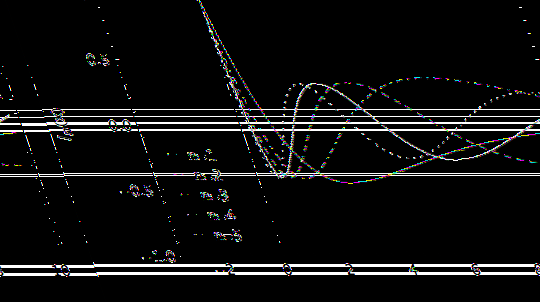
\includegraphics[max width=0.7\linewidth,keepaspectratio]{fig4_3.png}
\caption{前 5 个 Laguerre 正交函数 $\ell_n(x)$。}
\label{fig:4.3}
\end{figure}

在图~\ref{fig:4.3} 中我们给出了前几个 Laguerre 正交函数行为的一些例子。

\section{Bessel 函数}

我们已经引入了函数 $C_0(x)$，并证明它是 Laguerre 导数的本征函数。它是一族更一般的 Bessel 型函数的 0 阶。对 $C_0(x)$ 反复求导得到
\begin{equation}
\partial_x^n C_0(x) = (-1)^n C_n(x),
\label{eq:4.4.1}
\end{equation}
其中
\begin{equation}
C_n(x) = \sum_{r=0}^{\infty} \frac{(-1)^r x^r}{r!\,(n+r)!}.
\label{eq:4.4.2}
\end{equation}
函数 $C_n(x)$ 是 Tricomi 型的高阶 Bessel 型函数。

显然，下列递推关系由式~\eqref{eq:4.4.1} 推出：
\begin{equation}
\partial_x C_n(x) = -C_{n+1}(x),
\label{eq:4.4.3}
\end{equation}
而由式~\eqref{eq:4.4.2} 得到
\begin{equation}
n\,C_n(x) = C_{n-1}(x) - x\,\partial_x C_n(x)
= C_{n-1}(x) + x\,C_{n+1}(x).
\label{eq:4.4.4}
\end{equation}

由上述两个递推关系可以推导 Tricomi--Bessel 函数满足的微分方程。式~\eqref{eq:4.4.3}--\eqref{eq:4.4.4} 可以写成
\begin{equation}
\hat s_+ C_n(x) = C_{n+1}(x),
\qquad
\hat s_- C_n(x) = C_{n-1}(x),
\label{eq:4.4.5}
\end{equation}
其中
\begin{equation}
\hat s_+ = -\partial_x,
\qquad
\hat s_- = \hat n + x\partial_x.
\label{eq:4.4.6}
\end{equation}
算子 $\hat s_\pm$ 称为\emph{移位算子}，数算子 $\hat n$ 定义为
\begin{equation}
\hat n\,C_m(x) = m\,C_m(x).
\label{eq:4.4.7}
\end{equation}

$C_n(x)$ 满足的 ODE 由
\begin{equation}
\hat s_+ \hat s_- C_n(x) = C_n(x),
\label{eq:4.4.8}
\end{equation}
推出，它意味着
\begin{equation}
x\,C_n''(x) + (1+n)\,C_n'(x) + C_n(x) = 0.
\label{eq:4.4.9}
\end{equation}

还可以很容易地证明 Tricomi--Bessel 函数由生成函数
\begin{equation}
B(x,t) = \sum_{n=-\infty}^{\infty} t^n C_n(x)
= e^{\,t - x/t}.
\label{eq:4.4.10}
\end{equation}
确定。

此外，把式~\eqref{eq:4.4.4} 两边乘以 $t^{n-1}$ 得到
\begin{equation}
n\,t^{n-1} C_n = t^{n-1} C_{n-1} + \frac{x}{t^2}\,t^{n+1} C_{n+1},
\label{eq:4.4.11}
\end{equation}
由此可以推导 $B(x,t)$ 满足的微分方程：
\begin{equation}
\begin{cases}
\partial_t B(x,t) = \left(1 + \dfrac{x}{t^2}\right) B(x,t),\\[4pt]
B(x,0) = 1.
\end{cases}
\label{eq:4.4.12}
\end{equation}

Tricomi--Bessel 函数与普通柱 Bessel 函数由恒等式
\begin{equation}
C_n(x) = \left(\frac{x}{2}\right)^{-n} J_n\!\left(2\sqrt{x}\right),
\label{eq:4.4.13}
\end{equation}
联系，求逆得到
\begin{equation}
J_n(x) = \left(\frac{x}{2}\right)^{\!n}
C_n\!\left(\frac{x^2}{4}\right).
\label{eq:4.4.14}
\end{equation}

柱 Bessel 函数的性质可以直接由 Tricomi 函数的性质推得。兹总结如下。

\subsection*{Bessel 函数 $J_n(x)$：关键性质}

\begin{enumerate}
\item \textbf{级数展开}
\begin{equation}
J_n(x) = \sum_{r=0}^{\infty}
\frac{(-1)^r (x/2)^{n+2r}}{r!\,(n+r)!}.
\label{eq:4.4.15}
\end{equation}

\item \textbf{反射性质}
\begin{equation}
J_{-n}(x) = J_n(-x) = (-1)^n J_n(x).
\label{eq:4.4.16}
\end{equation}

\item \textbf{生成函数}
\begin{equation}
J(x,t) = \sum_{n=-\infty}^{\infty} t^n J_n(x)
= \exp\!\left[\frac{x}{2}\left(t - \frac{1}{t}\right)\right].
\label{eq:4.4.17}
\end{equation}

\item \textbf{递推关系}
\begin{align}
\partial_x J_n(x) &= \tfrac12\bigl(J_{n-1}(x) - J_{n+1}(x)\bigr),\\
n\,J_n(x) &= \tfrac{x}{2}\bigl(J_{n-1}(x) + J_{n+1}(x)\bigr).
\label{eq:4.4.18}
\end{align}

\item \textbf{Bessel 微分方程}
\begin{equation}
x^2 J_n''(x) + x\,J_n'(x) + (x^2 - n^2)\,J_n(x) = 0.
\label{eq:4.4.19}
\end{equation}

\item \textbf{Jacobi 生成函数}
\begin{equation}
\sum_{n=-\infty}^{\infty} e^{in\vartheta} J_n(x) = e^{i x\sin\vartheta}.
\label{eq:4.4.20}
\end{equation}

\item \textbf{积分表示}
\begin{equation}
J_n(x) = \frac{1}{\pi}\int_0^{\pi}
\cos\!\bigl(x\sin\vartheta - n\vartheta\bigr)\,d\vartheta.
\label{eq:4.4.21}
\end{equation}
\end{enumerate}

\begin{figure}[h]
\centering
\begin{minipage}{0.48\linewidth}
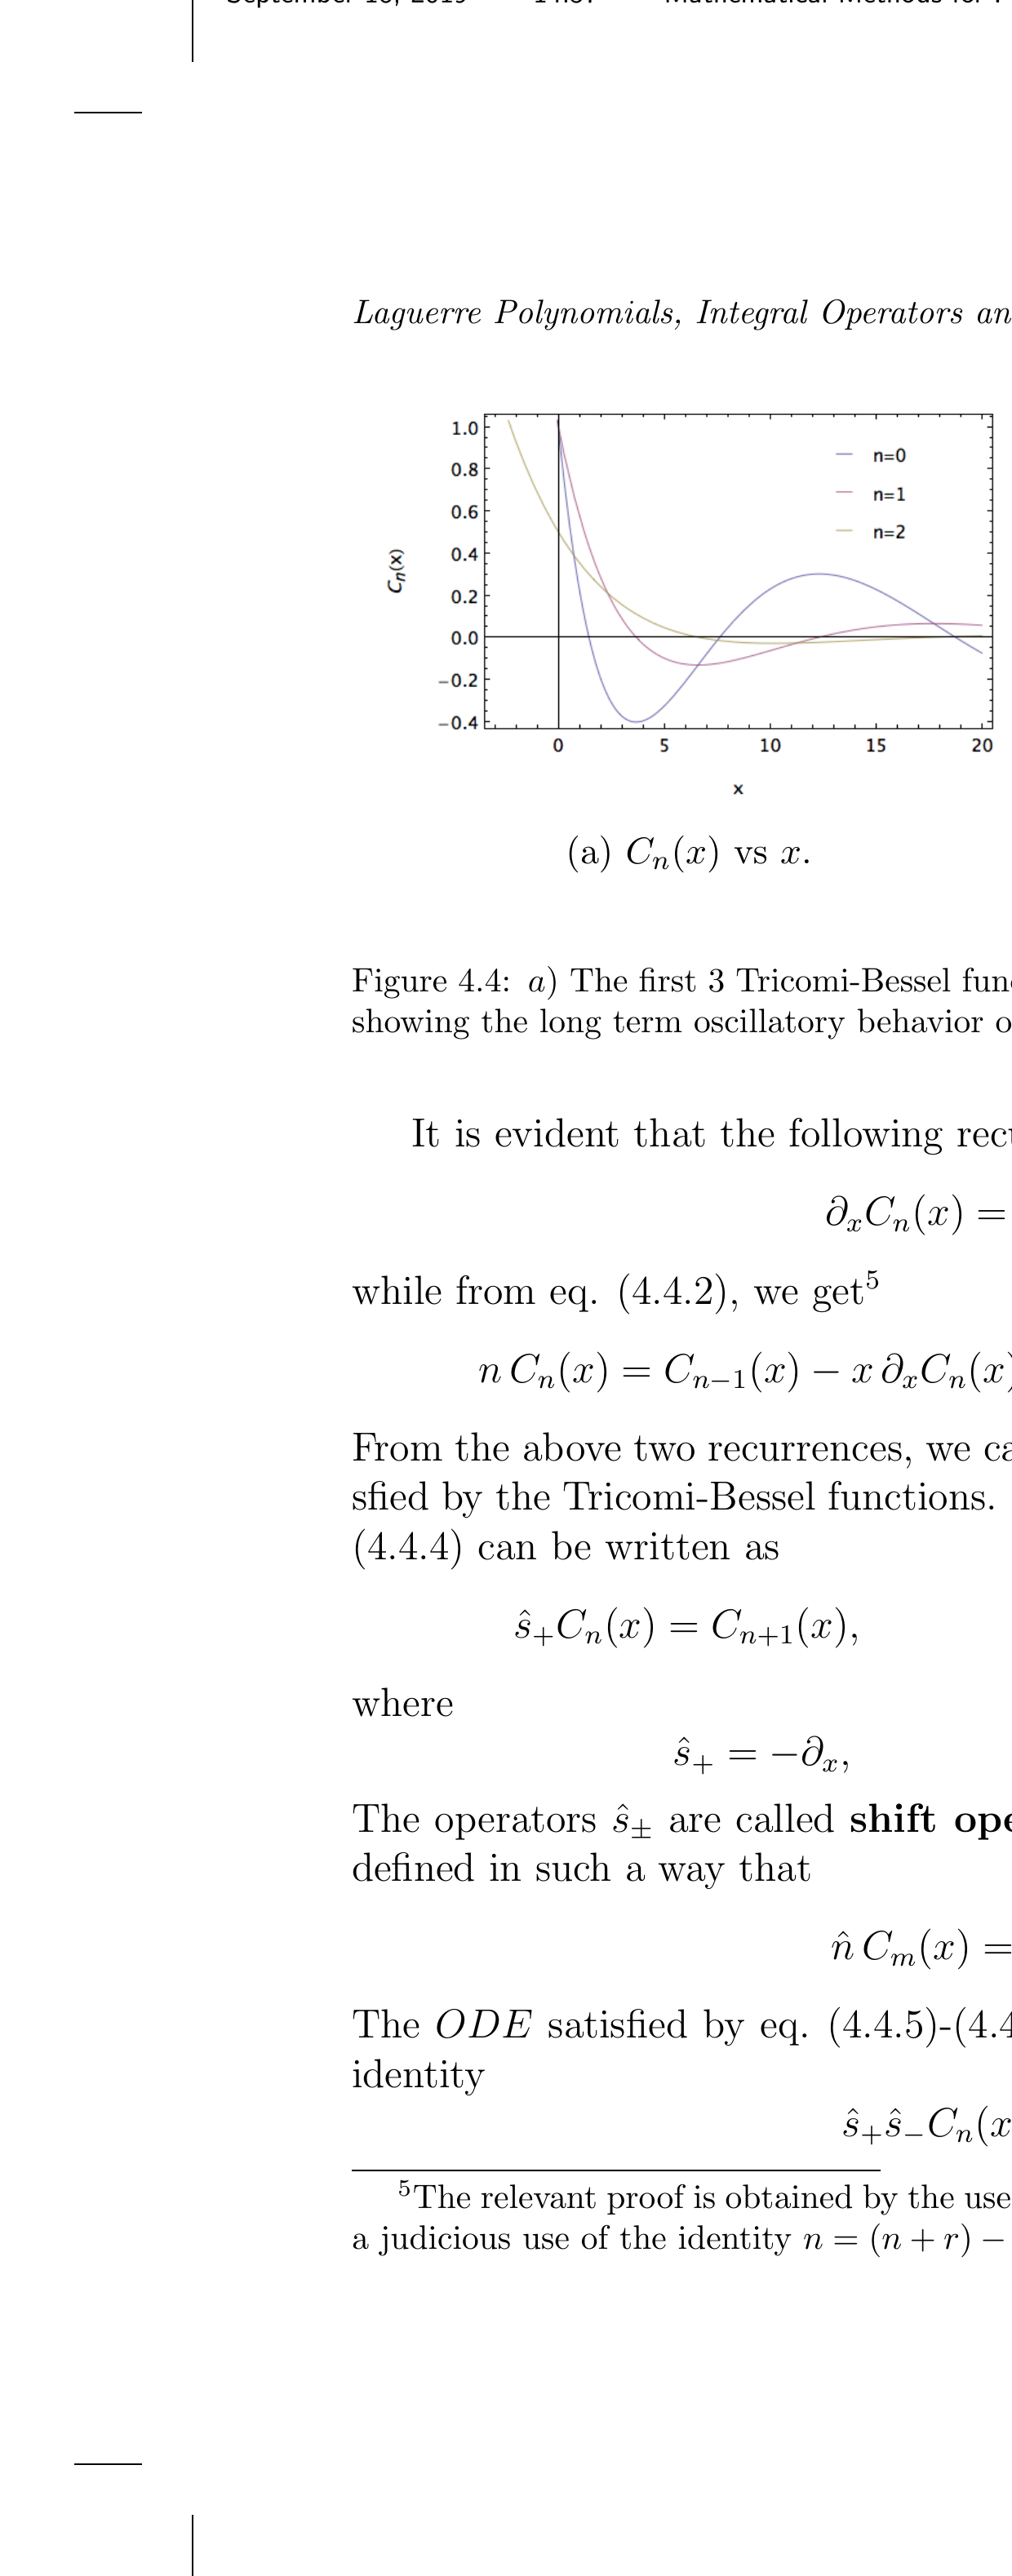
\includegraphics[max width=\linewidth,keepaspectratio]{fig4_4a.png}
\subcaption{$C_n(x)$ 关于 $x$ 的图形。}
\end{minipage}\hfill
\begin{minipage}{0.48\linewidth}
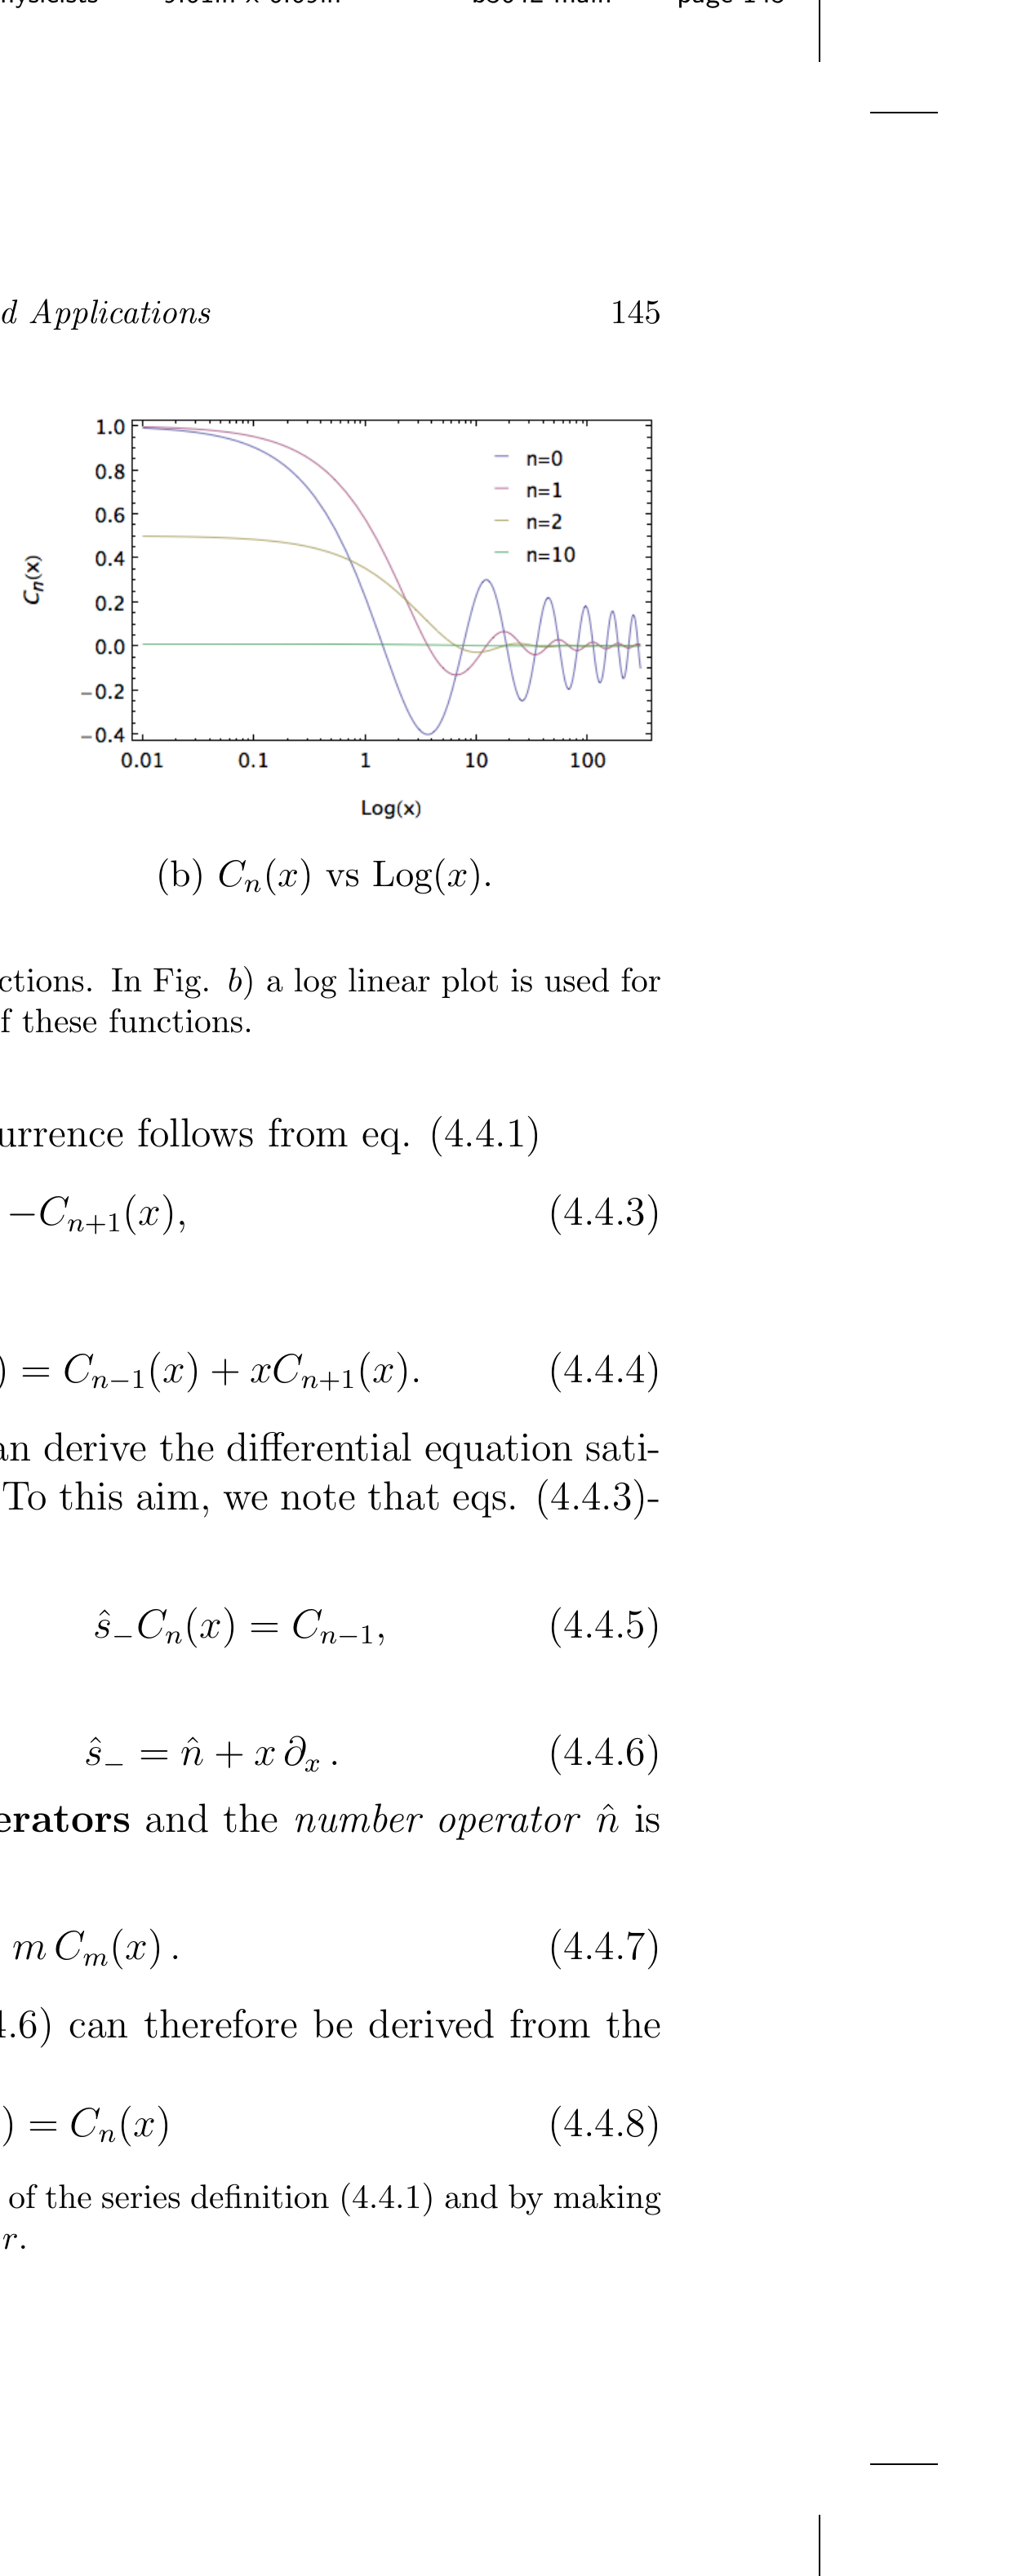
\includegraphics[max width=\linewidth,keepaspectratio]{fig4_4b.png}
\subcaption{$C_n(x)$ 关于 $\log x$ 的图形（半对数图）。}
\end{minipage}
\caption{Tricomi--Bessel 函数 $C_n(x)$：(a) 前 3 个函数；(b) 对数-线性图，展示长期振荡行为。}
\label{fig:4.4}
\end{figure}

\begin{figure}[h]
\centering
\setlength{\fboxsep}{6pt}\framebox[\textwidth]{\rule{0pt}{1.2cm}
  \textbf{图\,4.5（占位）：}前三个 Tricomi--Bessel 函数 $C_n(x)$ 与 Bessel 函数 $J_n(x)$ 的比较。}
\caption{前三个 Tricomi--Bessel 函数 $C_n(x)$ 与 Bessel 函数 $J_n(x)$ 的比较。}
\label{fig:4.5}
\end{figure}

\section{连带 Laguerre 多项式}

在前几节中，我们处理了 Laguerre 多项式理论，并看到它们的生成函数与 0 阶 Tricomi 函数相关。我们可能想知道，按如下方式修改生成函数能否得到新的 LP 族：
\begin{equation}
\sum_{n=0}^{\infty} \frac{t^n}{(n+m)!}\,L_n^{(m)}(x,y)
= e^{yt}\,C_m(xt).
\label{eq:4.5.1}
\end{equation}

可以直接验证
\begin{equation}
L_n^{(m)}(x,y)
= \frac{(n+m)!}{n!}\,
\sum_{r=0}^{n} \frac{(-1)^r y^{\,n-r} x^r}{(n-r)!\,(m+r)!\,r!}.
\label{eq:4.5.2}
\end{equation}

上述定义也与算子形式
\begin{equation}
L_n^{(m)}(x,y)
= (1 - y\partial_x)^m (y - \hat D_x^{-1})^n 1,
\label{eq:4.5.3}
\end{equation}
相容，据此可以推导这一 LP 推广的多数性质，例如生成函数
\begin{equation}
\sum_{n=0}^{\infty} t^n L_n^{(m)}(x,y)
= \frac{1}{(1-yt)^{m+1}}\,\exp\!\left(-\frac{xt}{1-yt}\right).
\label{eq:4.5.4}
\end{equation}

对于连带 Laguerre 多项式，Laguerre 导数即满足
\begin{equation}
{}^{(m)}\!\hat{\mathcal L}\!\hat D_x\,
L_n^{(m)}(x,y) = (n+m)\,L_{n-1}^{(m)}(x,y),
\label{eq:4.5.5}
\end{equation}
的算子为
\begin{equation}
{}^{(m)}\!\hat{\mathcal L}\!\hat D_x
= -\partial_x \hat D_x^{-1} - m\,\partial_x.
\label{eq:4.5.6}
\end{equation}

相应的 ODE 可以由关系
\begin{equation}
L_n(x,y) = \frac{n!}{(n+m)!}\,\partial_x^m
\bigl[x^m L_n^{(m)}(x,y)\bigr].
\label{eq:4.5.7}
\end{equation}
十分简单地推出。

利用乘法算子与普通（$m=0$）情形具有相同形式的事实，得到
\begin{equation}
y\,x\,\partial_x^2 L_n^{(m)}
+ \bigl((1+m)y - x\bigr)\partial_x L_n^{(m)}
+ n\,L_n^{(m)} = 0.
\label{eq:4.5.8}
\end{equation}

我们现在已具备足够的能力来证明函数集（$y=1$）
\begin{equation}
\ell_n^{(m)}(x) = \sqrt{\frac{n!}{(n+m)!}}\,e^{-x/2} x^{m/2}
L_n^{(m)}(x)
\label{eq:4.5.9}
\end{equation}
是正交的。这些函数满足的微分方程为
\begin{equation}
x\,\ell_n^{(m)\prime\prime}
+ \ell_n^{(m)\prime}
+ \left[n + \frac{1}{2} - \frac{x}{4} - \frac{m(m-2x)}{4x}\right]
\ell_n^{(m)} = 0.
\label{eq:4.5.10}
\end{equation}

上述函数在不同 $m$ 值下行为的例子见图~\ref{fig:4.6}。

\begin{figure}[h]
\centering
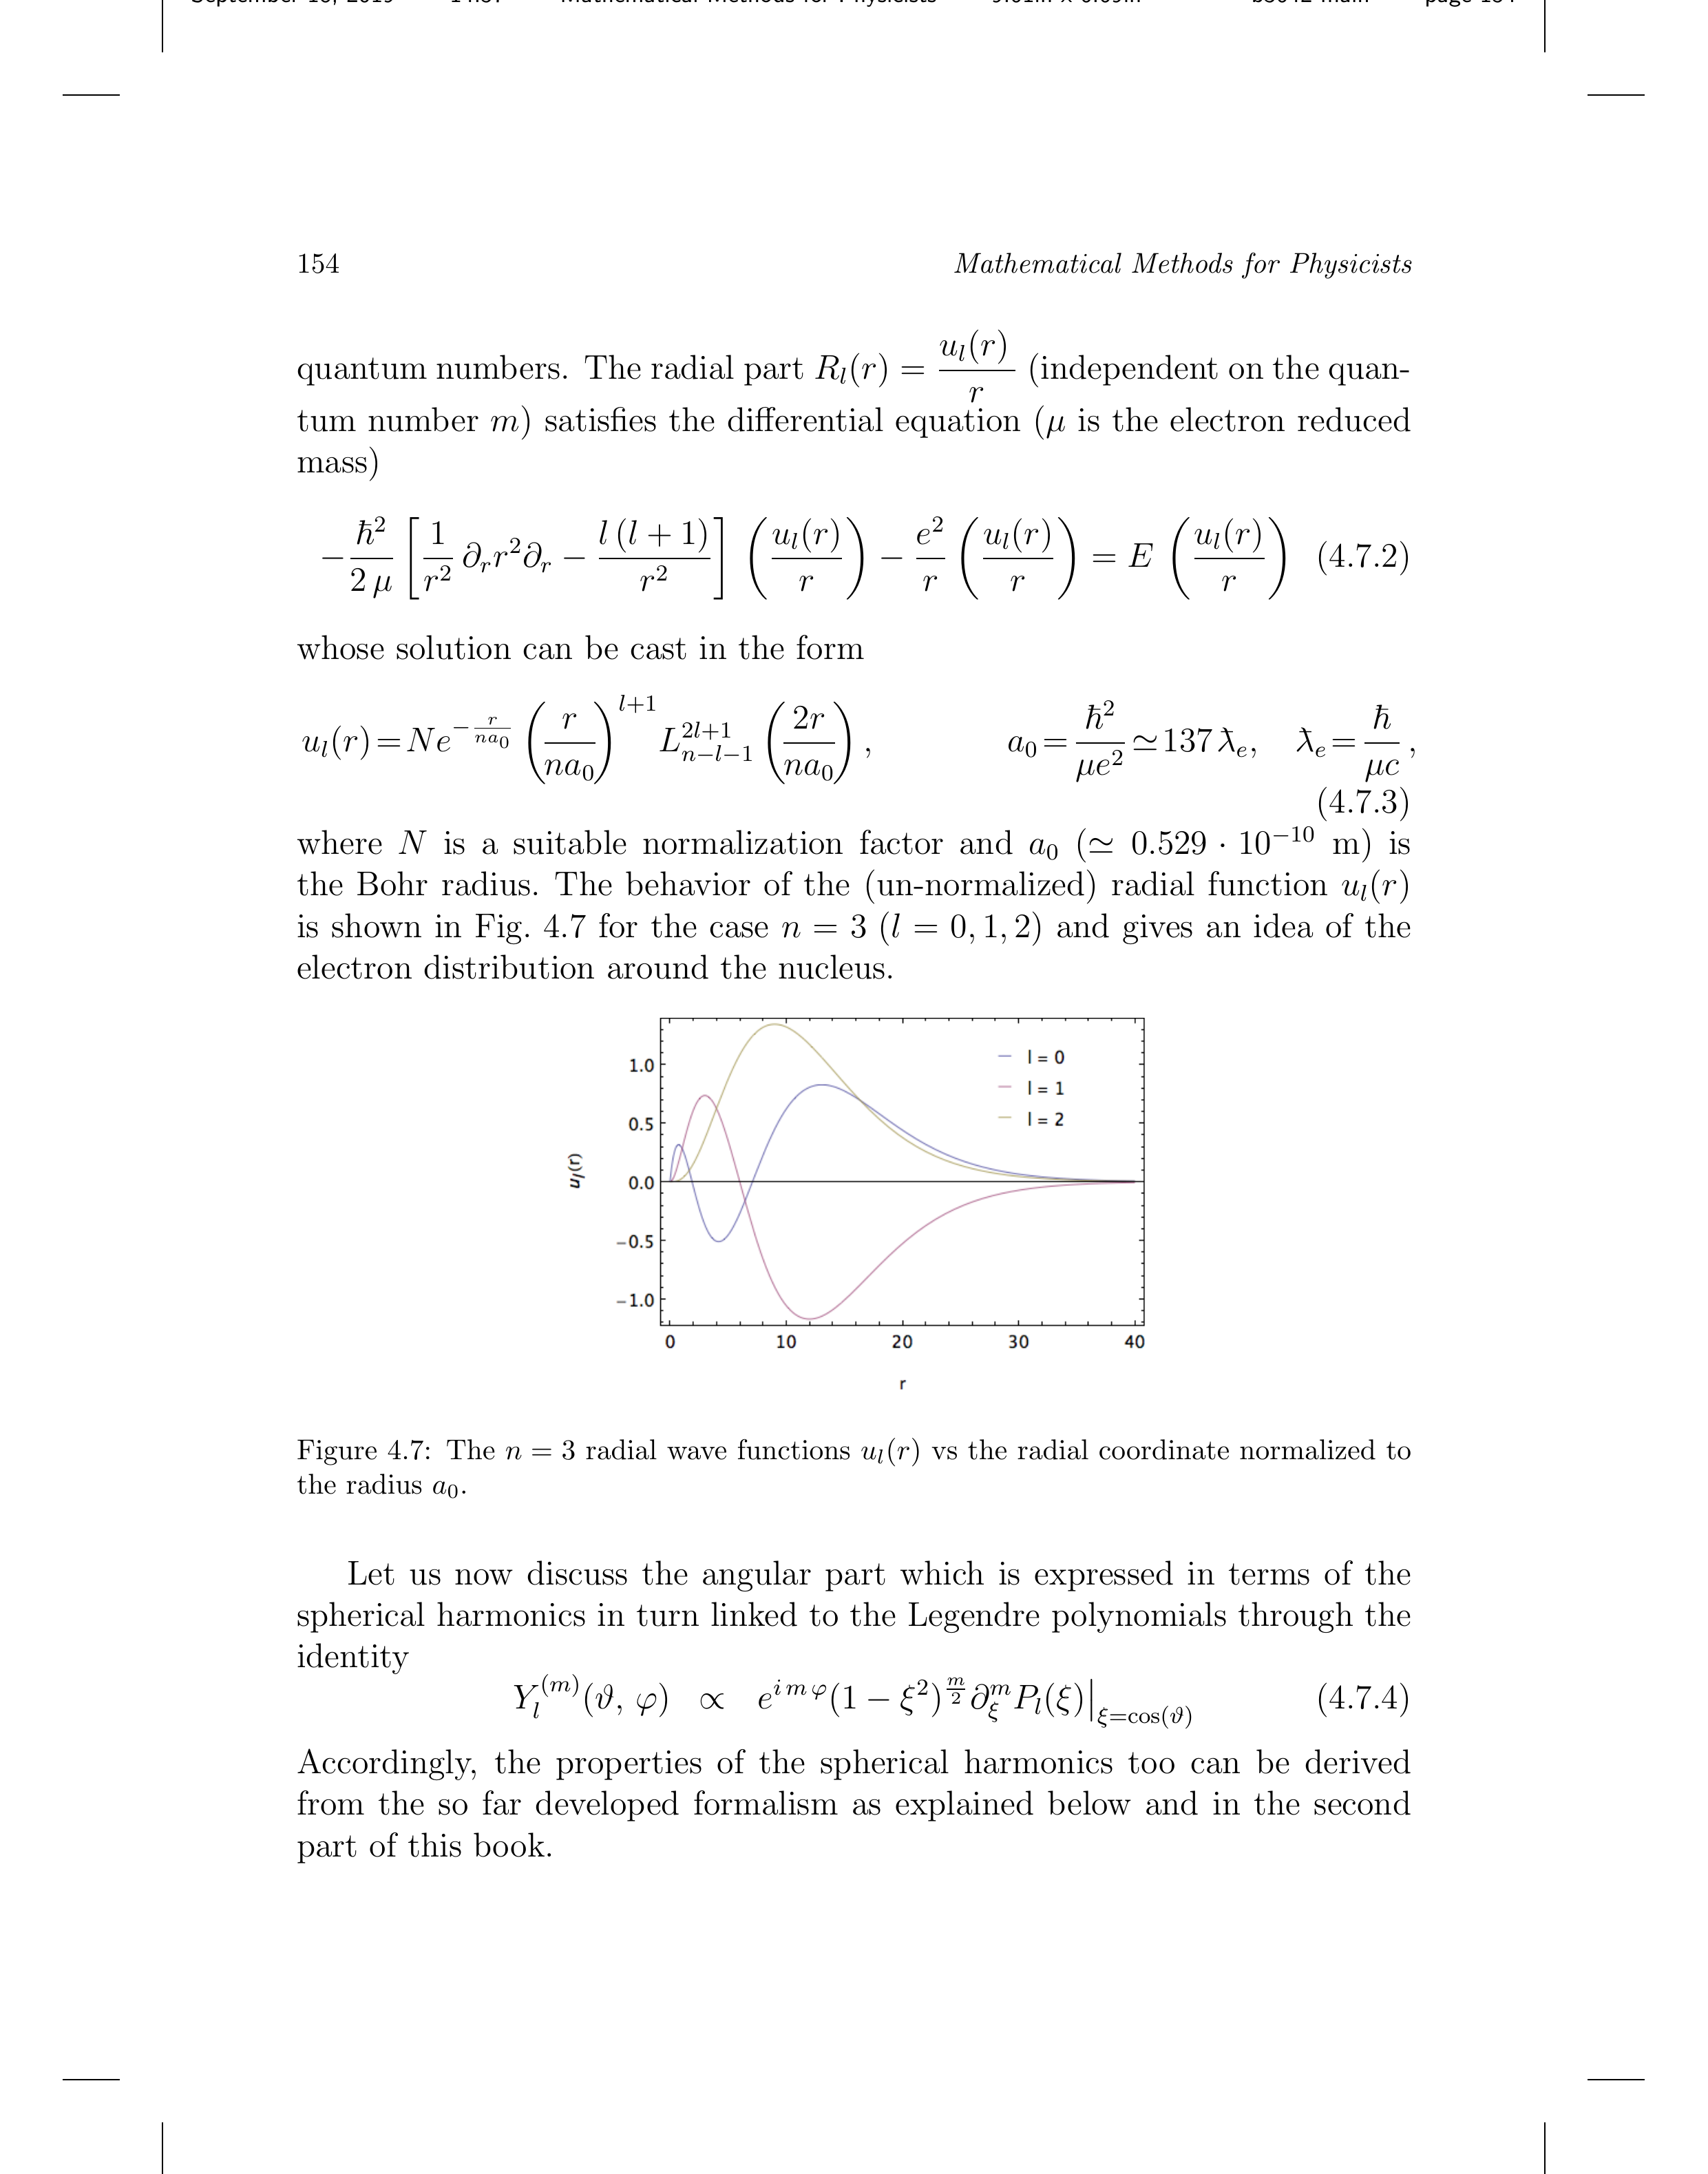
\includegraphics[max width=0.7\linewidth,keepaspectratio]{fig4_6.png}
\caption{不同 $m$ 与 $n$ 值下的 Laguerre 正交函数 $\ell_n^{(m)}(x)$：(a) $n=3,\ m=0,4$；(b) $n=2,\ m=0,4$。}
\label{fig:4.6}
\end{figure}

\section{Legendre 多项式}

我们声称在定义 Laguerre 或 Hermite 函数时使用额外变量特别有用，因为它为形式体系提供了额外的自由度。对于 Legendre 多项式 $P_n(x)$，生成函数为
\begin{equation}
\frac{1}{\sqrt{1-2xt+t^2}} = \sum_{n=0}^{\infty} t^n P_n(x),
\qquad |t|<1.
\label{eq:4.6.1}
\end{equation}

Legendre 多项式满足正交关系
\begin{equation}
\int_{-1}^{1} P_n(x)\,P_m(x)\,dx = \frac{2}{2n+1}\,\delta_{nm},
\label{eq:4.6.2}
\end{equation}
并且是 Legendre 微分方程
\begin{equation}
(1-x^2)P_n''(x) - 2x\,P_n'(x) + n(n+1)\,P_n(x) = 0.
\label{eq:4.6.3}
\end{equation}
的解。

\section{杂项应用与评论}

Laguerre 与 Bessel 函数的应用包括多极展开、散射理论中的球 Bessel 函数，以及利用生成函数计算原子物理中的径向积分。连带 Laguerre 函数自然出现在氢原子径向波函数中，其中参数 $m$ 与轨道角动量量子数 $\ell$ 相关。

关于 Bessel 函数及其应用的进一步说明见第 8--9 章。

\section{Appell 多项式与最后评论}

Appell 多项式 $A_n(x)$ 满足 $A_n'(x) = n\,A_{n-1}(x)$，构成第 9 章所处理 umbral 演算的支柱。本章引入的双变量 Laguerre 多项式确实是 Appell 分类的一个特例。

在第 8 章我们将看到，同样的结果如何能通过基于``umbral''方法的互补技术实现。

\section*{参考文献}

\begin{thebibliography}{99}

\bibitem{Lag1}
G. Szeg\H{o}, \emph{Orthogonal Polynomials}, 4th ed.,
Amer. Math. Soc. Colloq. Publ., Vol.~23, Providence, RI, 1975.

\bibitem{Lag2}
M. Abramowitz, I.A. Stegun (Eds.),
\emph{Handbook of Mathematical Functions},
Dover, New York, 1965.

\bibitem{Lag3}
W. Magnus, F. Oberhettinger, R.P. Soni,
\emph{Formulas and Theorems for the Special Functions of Mathematical Physics},
3rd ed., Springer, Berlin, 1966.

\bibitem{Lag4}
G. Dattoli, P.L. Ottaviani, A. Torre, L. Vazquez,
``Evolution operator equations, integration with algebraic and finite difference
methods: applications to physical problems in classical and quantum
mechanics,''
\emph{Riv. Nuovo Cimento} \textbf{20}, pp.~1--133, 1997.

\bibitem{Lag5}
G. Dattoli, S. Lorenzutta, A. Torre,
``Theory of multi-index multivariable Bessel functions and Hermite
polynomials,''
\emph{Matematiche} (Catania) \textbf{52}, pp.~179--197, 1997.

\bibitem{Lag6}
G. Dattoli, H.M. Srivastava, K. Zhukovsky,
``Orthogonality properties of the Hermite and related polynomials,''
\emph{J. Comput. Appl. Math.} \textbf{182}(1), pp.~165--172, 2005.

\bibitem{Lag7}
F.G. Tricomi,
\emph{Funzioni Ipergeometriche Confluenti},
Cremonese, Roma, 1954.

\bibitem{Lag8}
N.N. Lebedev,
\emph{Special Functions and Their Applications},
Dover Books on Mathematics, 1972.

\end{thebibliography}

% ch5.tex — 练习与补充 I（中文版）
\chapter{练习与补充 I}

\section{Pauli 与 Jones 矩阵以及 Mueller 演算}

Jones 矢量描述完全偏振光；单色平面波的 Jones 矢量为
\begin{equation}
\vect{E} = \begin{pmatrix} E_x \\ E_y \end{pmatrix} e^{i(kz-\omega t)},
\label{eq:5.1.1}
\end{equation}
作用其上的任何无损耗光学元件都由一个 $2\times2$ 幺正矩阵（Jones 矩阵）表示。Pauli 矩阵构成一个方便的基：
\begin{equation}
\hat J = c_0\hat 1 + c_1\hat\sigma_x + c_2\hat\sigma_y + c_3\hat\sigma_z,
\qquad |c_0|^2+|c_1|^2+|c_2|^2+|c_3|^2 = 1.
\label{eq:5.1.2}
\end{equation}

对于部分偏振光，使用\emph{Stokes 参数} $S_0,S_1,S_2,S_3$，它们组成 Stokes 矢量，由 $4\times4$ 的 Mueller 矩阵变换。与 Jones 演算的联系是
\begin{equation}
\vect S = \begin{pmatrix} S_0\\S_1\\S_2\\S_3 \end{pmatrix}
= \begin{pmatrix}
E_xE_x^*+E_yE_y^*\\
E_xE_x^*-E_yE_y^*\\
E_xE_y^*+E_yE_x^*\\
i(E_xE_y^*-E_yE_x^*)
\end{pmatrix}.
\label{eq:5.1.3}
\end{equation}

\begin{exercise}
证明快轴与 $x$ 轴成 $45^\circ$ 的四分之一波片对应 Jones 矩阵
$\frac{1}{\sqrt2}\mat{1&-i\\-i&1}$
与 Mueller 矩阵
$\frac12\mat{1&0&0&1\\0&0&0&0\\0&0&1&0\\1&0&0&0}$。
\end{exercise}

\section{磁透镜与矩阵描述}

均匀磁场 $\vect B = B\hat z$ 中的带电粒子作回旋运动。焦距为 $f$ 的磁\emph{透镜}在长度为 $L$ 的漂移段中由传输矩阵
\begin{equation}
\hat M = \hat O(L)\,\hat F(f) =
\mat{1&L\\0&1}\mat{1&0\\-1/f&1}
= \mat{1-L/f & L \\ -1/f & 1},
\label{eq:5.2.1}
\end{equation}
描述，重现了第 1 章的薄透镜 ABCD 定律。

对于四极磁透镜，聚焦平面中的传输矩阵为
\begin{equation}
\hat M_q = \mat{\cos\sqrt{k}L & \frac{1}{\sqrt{k}}\sin\sqrt{k}L
           \\ -\sqrt{k}\sin\sqrt{k}L & \cos\sqrt{k}L},
\qquad k = \frac{qB_0}{p},
\label{eq:5.2.2}
\end{equation}
其中 $p$ 是粒子动量。FODO 单元（聚焦--漂移--散焦--漂移）是大多数加速器格点（lattice）的构造单元。

\begin{exercise}
对于漂移长度 $L$ 与四极长度 $\ell$ 均相等的 FODO 单元，证明单元矩阵为
$\hat M_{\rm cell}=\hat O(L)\hat Q_f(\ell)\hat O(2L)\hat Q_d(\ell)\hat O(L)$，
且稳定性要求 $|{\rm Tr}\,\hat M_{\rm cell}/2|<1$。
\end{exercise}

\section{矩阵形式体系杂谈与演化问题的求解}

\subsection{矩阵与四元数}

四元数 $q=q_0+\vect q\cdot\vect\sigma$（其中 $\vect\sigma=(\hat\sigma_x,\hat\sigma_y,\hat\sigma_z)$）映射到 $SU(2)$，并通过
\begin{equation}
\vect r' = q\,\vect r\,\bar q, \qquad \bar q = q_0 - \vect q\cdot\vect\sigma.
\label{eq:5.3.1}
\end{equation}
描述三维旋转。四元数共轭对应逆旋转。

\subsection{演化问题的矩阵求解}

第 1 章的解缠恒等式可推广到四元数/旋转演化。对于含时扭矩 $\vect\Omega(t)$，
\begin{equation}
\hat U(t) = \exp\!\left(-i\int_0^t \vect\Omega(t')\cdot\frac{\vect\sigma}{2}\,dt'\right)
\label{eq:5.3.2}
\end{equation}
是 $i\partial_t\vect\sigma = \vect\Omega\times\vect\sigma$ 的解。

\section{Lorentz 变换}

$(ct,x)$ 平面内速度为 $v$ 的 Lorentz boost 为
\begin{equation}
\begin{pmatrix} ct'\\x' \end{pmatrix}
=
\mat{\gamma&-\beta\gamma\\-\beta\gamma&\gamma}
\begin{pmatrix} ct\\x \end{pmatrix},
\qquad
\gamma=\frac{1}{\sqrt{1-\beta^2}},\ \beta=\frac{v}{c}.
\label{eq:5.4.1}
\end{equation}
这是快度（rapidity）为 $\alpha$ 的双曲旋转：
$\beta=\tanh\alpha$，$\gamma=\cosh\alpha$，$\beta\gamma=\sinh\alpha$。

boost 可以写成指数形式：
\begin{equation}
\hat\Lambda(\beta) = \exp(-\alpha\hat K_x), \qquad
\hat K_x = \mat{0&-1\\-1&0},
\label{eq:5.4.2}
\end{equation}
且 $[\hat K_x,\hat J_y]=i\hat K_z$ 等等，封闭 Lorentz 代数的对易子。

\begin{exercise}
验证 $\hat\Lambda(\beta_1)\hat\Lambda(\beta_2)\neq\hat\Lambda(\beta_2)\hat\Lambda(\beta_1)$，
并推导速度合成公式
$v_{12}=(v_1+v_2)/(1+v_1v_2/c^2)$。
\end{exercise}

\section{双曲三角学与狭义相对论}

$\alpha=\operatorname{artanh}\beta$ 的双曲旋转 $\hat R_h(\alpha)$ 给出 boost 矩阵，把第 1 章的双曲单位 $\hat h$ 与快度联系起来。关键恒等式：
\begin{align}
\cosh(\alpha_1+\alpha_2) &= \cosh\alpha_1\cosh\alpha_2 + \sinh\alpha_1\sinh\alpha_2,\\
\sinh(\alpha_1+\alpha_2) &= \sinh\alpha_1\cosh\alpha_2 + \cosh\alpha_1\sinh\alpha_2.
\label{eq:5.5.1}
\end{align}

不变量隔 $ds^2 = -c^2dt^2 + dx^2+dy^2+dz^2$ 被所有 Lorentz 变换保持。固有时为
$d\tau = dt/\gamma$。

\begin{exercise}
证明以快度 $\alpha$ 运动的源发出的光的 Doppler 频移为 $\omega'=\omega e^{\alpha}$（纵向情形）。
\end{exercise}

\section{略谈椭圆函数}

Jacobi 椭圆函数 $\sn u$、$\cn u$、$\dn u$（参数 $k$，$0\le k\le1$）以如下形式求解非线性摆方程
\begin{equation}
\theta'' + \omega^2\sin\theta = 0
\label{eq:5.6.1}
\end{equation}
\begin{equation}
\theta(u) = 2\arcsin\bigl(k\,\sn(u;k)\bigr), \qquad u = \omega t.
\label{eq:5.6.2}
\end{equation}

它们满足
\begin{align}
\sn^2 u + \cn^2 u &= 1,\\
\dn^2 u + k^2\sn^2 u &= 1,\\
\frac{d}{du}\sn u &= \cn u\,\dn u.
\label{eq:5.6.3}
\end{align}

加法公式：
\begin{align}
\sn(u+v) &= \frac{\sn u\,\cn v\,\dn v + \sn v\,\cn u\,\dn u}
                  {1-k^2\sn^2 u\,\sn^2 v},\\
\cn(u+v) &= \frac{\cn u\,\cn v - \sn u\,\dn u\,\sn v\,\dn v}
                {1-k^2\sn^2 u\,\sn^2 v},\\
\dn(u+v) &= \frac{\dn u\,\dn v - k^2\sn u\,\cn u\,\sn v\,\cn v}
                {1-k^2\sn^2 u\,\sn^2 v}.
\label{eq:5.6.4}
\end{align}

周期性：$\sn(u+4K)=\sn u$，$\cn(u+4K)=\cn u$，$\dn(u+2K)=\dn u$，
其中 $K(k)=\int_0^{\pi/2}(1-k^2\sin^2\phi)^{-1/2}d\phi$ 是第一类完全椭圆积分。

极限情形：
\begin{align}
k\to0:&\quad \sn u\to\sin u,\ \cn u\to\cos u,\ \dn u\to1,\\
k\to1:&\quad \sn u\to\tanh u,\ \cn u\to\sech u,\ \dn u\to\sech u.
\label{eq:5.6.5}
\end{align}

\begin{exercise}
推导倍角公式
\begin{align}
\sn(2u) &= \frac{2\sn u\,\cn u\,\dn u}{1-k^2\sn^4 u},\\
\cn(2u) &= \frac{\cn^2 u - \sn^2 u\,\dn^2 u}{1-k^2\sn^4 u},\\
\dn(2u) &= \frac{\dn^2 u - k^2\sn^2 u\,\cn^2 u}{1-k^2\sn^4 u}.
\end{align}
\end{exercise}

\begin{exercise}
证明 $\sn(u+K) = \cn u/\dn u$，且
$\cn(u+K) = -\sqrt{1-k^2}\,\sn u/\dn u$。
\end{exercise}

\section{结论性评论}

第 1--2 章的矩阵方法可以统一地推广到 Lorentz、旋量与四元数形式体系。双曲/椭圆函数提供了 Euler 角与快度参数只能微扰地参数化的那些问题的精确（非微扰）解。在接下来的章节中，我们将转向 Fourier 方法与特殊函数，它们在动量空间中使同样的这些问题对角化。

% 本章图形
\begin{figure}[h]
\centering
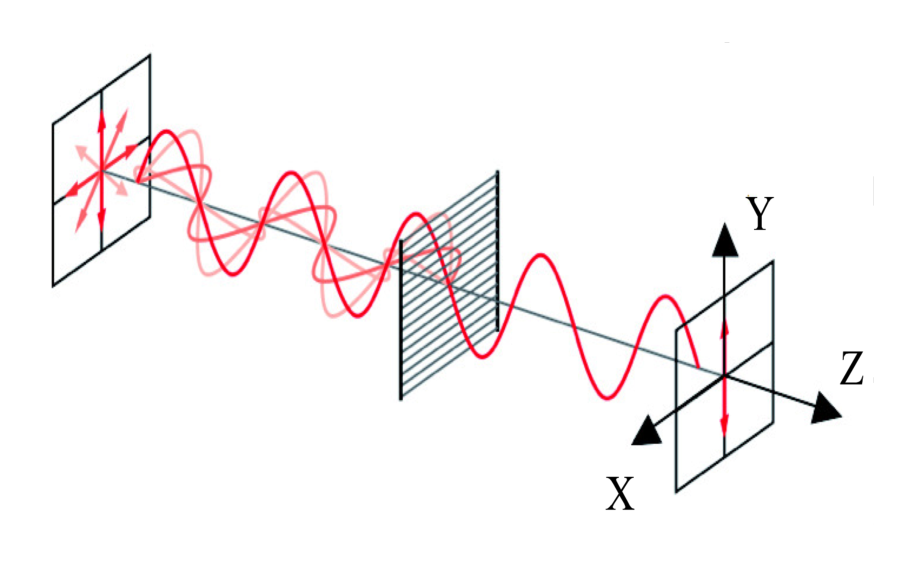
\includegraphics[max width=0.85\linewidth,keepaspectratio]{fig5_1.png}
\caption{Jones 矢量：Poincar\'e 球上的偏振态。}
\label{fig:5.1}
\end{figure}

\begin{figure}[h]
\centering
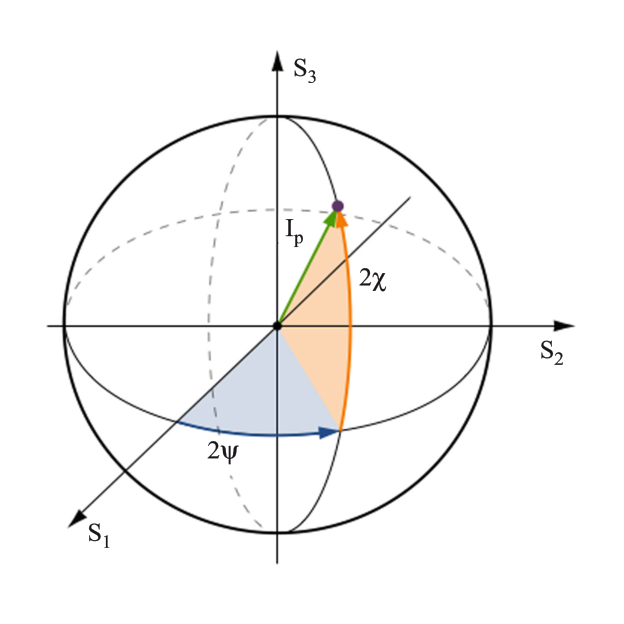
\includegraphics[max width=0.85\linewidth,keepaspectratio]{fig5_3.png}
\caption{Stokes 参数与 Poincar\'e 球表示。}
\label{fig:5.3}
\end{figure}

\begin{figure}[h]
\centering
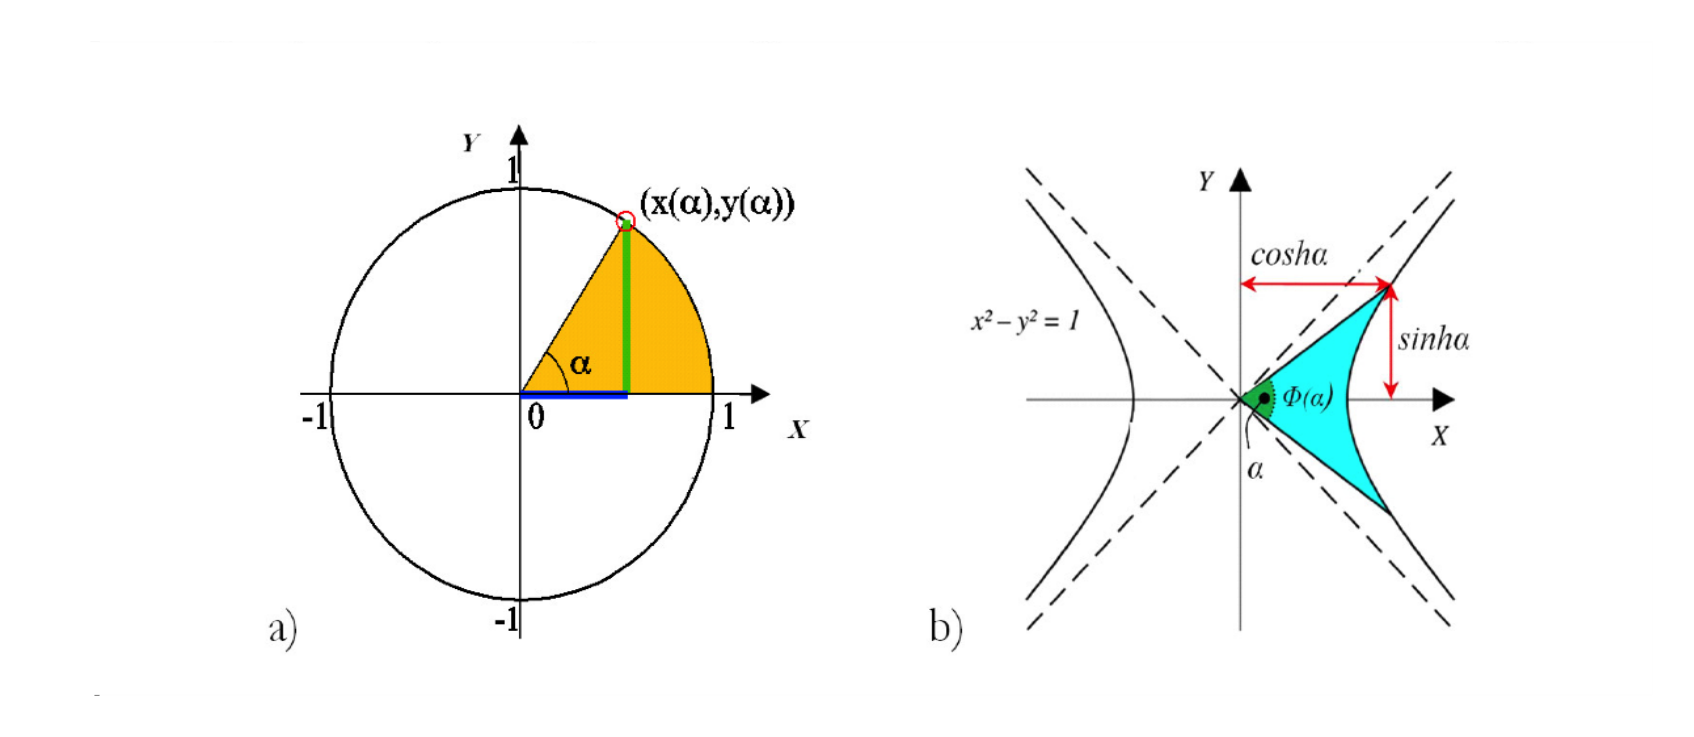
\includegraphics[max width=0.85\linewidth,keepaspectratio]{fig5_16.png}
\caption{椭圆函数：不同 $k$ 下 $\sn$、$\cn$、$\dn$ 关于 $u$ 的图形。}
\label{fig:5.16}
\end{figure}

\begin{figure}[h]
\centering
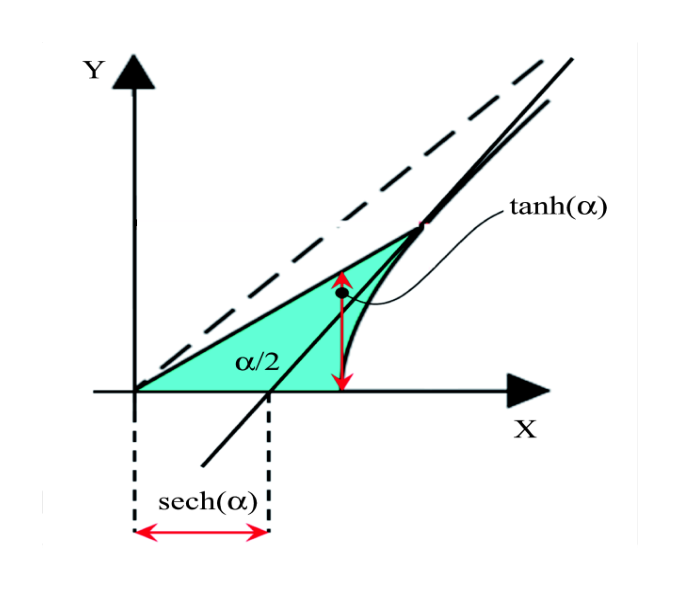
\includegraphics[max width=0.85\linewidth,keepaspectratio]{fig5_17.png}
\caption{Jacobi 椭圆函数的加法定理。}
\label{fig:5.17}
\end{figure}

% ch6.tex — 练习与补充 II（中文版）
\chapter{练习与补充 II}

\section{常微分方程与矩阵}

二阶 ODE $y''+\omega^2 y=\beta$ 映射为 $\dot{\vect z}=\hat M\vect z+\vect\phi$，其中
$\hat M=\mat{0&-\omega^2\\1&0}$，回到第 2 章的谐振子矩阵。通解为
\begin{equation}
\vect z(t) = e^{\hat M t}\vect z(0) + \int_0^t e^{\hat M(t-t')}\vect\phi\,dt'.
\label{eq:6.1.1}
\end{equation}

对于 $\vect\phi=\vect 0$ 且 $\hat M$ 为常数，
\begin{equation}
e^{\hat M t} =
\mat{\cos(\omega t)&-\omega\sin(\omega t)\\
     \frac{1}{\omega}\sin(\omega t)&\cos(\omega t)},
\label{eq:6.1.2}
\end{equation}
与第 2 章推导的结果完全相同。

\begin{exercise}
用矩阵方法求解 $y''+2\zeta\omega_0 y'+\omega_0^2 y = F_0\cos(\Omega t)$，并推导共振曲线。
\end{exercise}

\section{Crofton--Glaisher 恒等式与热型方程}

Crofton 恒等式
$e^{\xi\hat A}\hat B = \hat B e^{\xi\hat A} + \xi[\hat A,\hat B]e^{\xi\hat A}$
应用于热多项式给出 Glaisher 恒等式
\begin{equation}
e^{at\partial_x^2}\,e^{-x^2}
= \frac{1}{\sqrt{1+4at}}\;
\exp\!\left(-\frac{x^2}{1+4at}\right).
\label{eq:6.2.1}
\end{equation}

一个推广：对于热型方程
$\partial_t F = a\,\partial_x^2 F$ 且 $F(x,0)=x^n$，
\begin{equation}
F(x,t) = H_n(x,at) = n!\sum_{r=0}^{\lfloor n/2\rfloor}
\frac{x^{n-2r}(at)^r}{(n-2r)!\,r!}.
\label{eq:6.2.2}
\end{equation}

\begin{exercise}
证明 Crofton 恒等式 $e^{y\partial_x^m}f(x)=f(x+my\partial_x^{m-1})e^{y\partial_x^m}$，
并利用它推导 $\partial_x^{2m}$ 情形的广义 Glaisher 恒等式。
\end{exercise}

\section{Gamma 函数与定积分}

Euler 的 Gamma 函数：
\begin{equation}
\Gamma(z) = \int_0^\infty t^{z-1}e^{-t}\,dt, \qquad \Re(z)>0.
\label{eq:6.3.1}
\end{equation}

关键性质：
\begin{align}
\Gamma(z+1) &= z\,\Gamma(z),\\
\Gamma(\tfrac12) &= \sqrt{\pi},\\
\Gamma(n+1) &= n! \quad (n\in\mathbb N_0).
\label{eq:6.3.2}
\end{align}

Beta 函数：
\begin{equation}
B(p,q) = \int_0^1 t^{p-1}(1-t)^{q-1}dt
= \frac{\Gamma(p)\Gamma(q)}{\Gamma(p+q)}.
\label{eq:6.3.3}
\end{equation}

有用的积分：
\begin{equation}
\int_0^\infty x^{n}e^{-ax^2}dx =
\frac{\Gamma\!\left(\frac{n+1}{2}\right)}{2a^{(n+1)/2}},
\qquad a>0,\;n>-1.
\label{eq:6.3.4}
\end{equation}

\begin{exercise}
用 Beta 函数计算 $\int_0^{\pi/2}\sin^{2m}\theta\cos^{2n}\theta\,d\theta$。
\end{exercise}

\section{复变函数方法与积分计算}

对于在简单区域中解析的函数 $f(z)$，闭合路径积分消失（Cauchy 定理）。留数定理：
\begin{equation}
\oint_C f(z)\,dz = 2\pi i\sum_{z_k\in\text{int}(C)} \operatorname{Res}(f,z_k).
\label{eq:6.4.1}
\end{equation}

Jordan 引理：若 $f(z)$ 在上/下半平面内当 $|z|\to\infty$ 时一致趋于 $0$，则半圆弧积分消失。

\begin{exercise}
利用上半平面中的半圆围道计算 $\int_{-\infty}^{\infty}\frac{\cos(kx)}{1+x^2}\,dx$。
\end{exercise}

主值：对于实轴上 $x=\Omega$ 处的极点，
\begin{equation}
\mathcal P\int_{-\infty}^{\infty}\frac{\tilde\chi(\omega)}{\omega-\Omega}\,d\omega
= \lim_{\epsilon\to0}\left(
\int_{-\infty}^{\Omega-\epsilon}+\int_{\Omega+\epsilon}^{\infty}
\right)\frac{\tilde\chi(\omega)}{\omega-\Omega}\,d\omega.
\label{eq:6.4.2}
\end{equation}
$\omega=\Omega$ 周围的小半圆贡献为 $-i\pi\tilde\chi(\Omega)$。

\section{Fourier 变换}

定义：
\begin{equation}
\tilde f(k)=\int_{-\infty}^{\infty}f(x)\,e^{-ikx}\,dx,\qquad
f(x)=\frac{1}{2\pi}\int_{-\infty}^{\infty}\tilde f(k)\,e^{ikx}\,dk.
\label{eq:6.5.1}
\end{equation}

该变换把 $\partial_x$ 对角化为 $ik$，并把 PDE 化为 ODE。关键性质：
\begin{align}
\mathcal F[f'(x)] &= ik\,\tilde f(k),\\
\mathcal F[xf(x)] &= i\,\widetilde f\,'(k),\\
\mathcal F[f*g] &= \tilde f(k)\,\tilde g(k),
\label{eq:6.5.2}
\end{align}
其中 $(f*g)(x)=\int f(y)g(x-y)\,dy$。

Gauss 函数：
\begin{equation}
\mathcal F[e^{-ax^2}] = \sqrt{\frac{\pi}{a}}\,e^{-k^2/(4a)}.
\label{eq:6.5.3}
\end{equation}

\begin{exercise}
推导卷积定理，并用它通过 Fourier 变换求解
$y''+k_0^2y=s(x)$。
\end{exercise}

\section{Fourier 变换与微分方程的求解}

对于边界条件在无穷远的 $y''+k_0^2y=s(x)$，
\begin{equation}
\tilde y(k) = \frac{\tilde s(k)}{k_0^2-k^2},
\label{eq:6.6.1}
\end{equation}
逆变换给出 Green 函数解
\begin{equation}
y(x) = \int_{-\infty}^{\infty} G(x-\xi)\,s(\xi)\,d\xi,
\qquad G(x) = \frac{1}{2\pi}\int_{-\infty}^{\infty}
\frac{e^{ikx}}{k_0^2-k^2}\,dk.
\label{eq:6.6.2}
\end{equation}

在上/下半平面闭合围道给出
$G(x)=\frac{\sin(k_0|x|)}{k_0}$，回到第 8 章的 Green 函数。

\section{Fourier 型变换}

Hankel 变换（柱对称）：
\begin{equation}
\tilde f(\rho) = \int_0^\infty f(r)\,J_0(\rho r)\,r\,dr,
\qquad
f(r) = \int_0^\infty \tilde f(\rho)\,J_0(\rho r)\,\rho\,d\rho.
\label{eq:6.7.1}
\end{equation}

Mellin 变换：
\begin{equation}
\mathcal M[f](s) = \int_0^\infty f(x)\,x^{s-1}\,dx,
\qquad
f(x) = \frac{1}{2\pi i}\int_{c-i\infty}^{c+i\infty}
\mathcal M[f](s)\,x^{-s}\,ds.
\label{eq:6.7.2}
\end{equation}

Laplace 变换：
\begin{equation}
\mathcal L[f](s) = \int_0^\infty f(t)\,e^{-st}\,dt,
\qquad
\mathcal L[f'](s) = s\tilde f(s)-f(0).
\label{eq:6.7.3}
\end{equation}

\begin{exercise}
证明 Hankel 变换是柱坐标中的 Fourier 变换，并推导 $J_0$ 的正交关系。
\end{exercise}

% 图形
\begin{figure}[h]
\centering
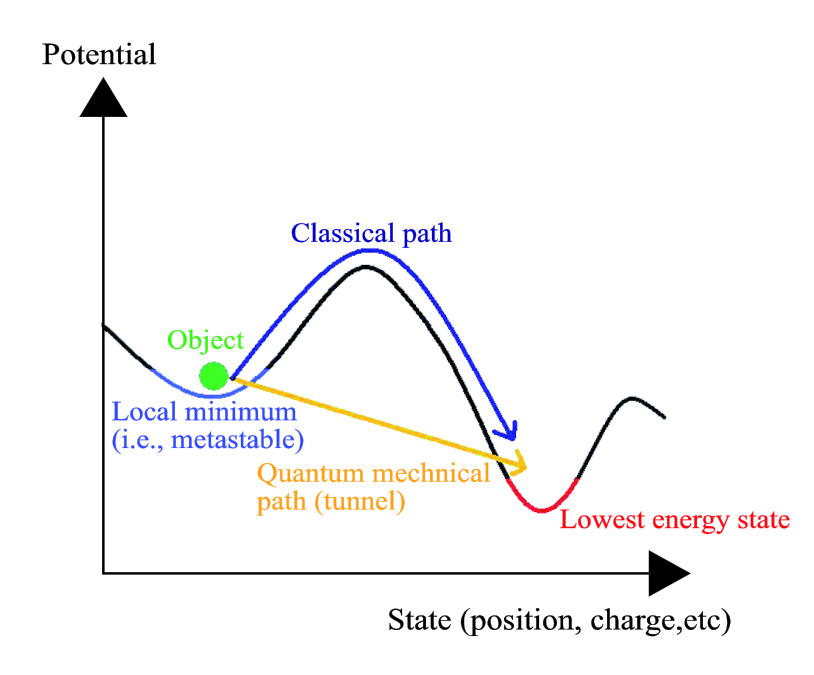
\includegraphics[max width=0.85\linewidth,keepaspectratio]{fig6_1.png}
\caption{Fourier 变换对：Gauss 函数及其变换。}
\label{fig:6.1}
\end{figure}

\begin{figure}[h]
\centering
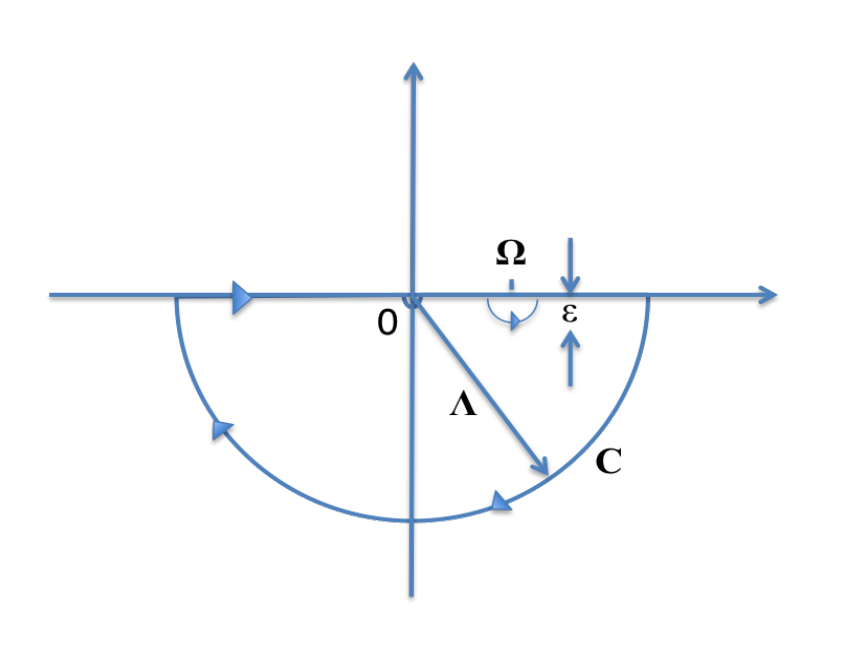
\includegraphics[max width=0.85\linewidth,keepaspectratio]{fig6_13.png}
\caption{主值积分在复 $\omega$ 平面中的积分围道。}
\label{fig:6.13}
\end{figure}

% ch7.tex — 练习与补充 III（中文版）
\chapter{练习与补充 III}

\section{Hermite 方程的第二个解}

Hermite 方程
\begin{equation}
y'' - 2xy' + 2ny = 0
\label{eq:7.1.1}
\end{equation}
对整数 $n$ 有多项式解 $H_n(x)$。第二个线性无关解（非多项式）为
\begin{equation}
y_2(x) = H_n(x)\int^x \frac{e^{t^2}}{H_n(t)^2}\,dt,
\label{eq:7.1.2}
\end{equation}
由降阶法得到。对 $n=0$，
$y_2(x)=\erfi(x)$（虚误差函数）。

\begin{exercise}
验证当 $y_1(x)=H_n(x)$ 时，\eqref{eq:7.1.2} 中的 $y_2(x)$ 满足 Hermite 方程。
\end{exercise}

\section{高阶 Hermite 多项式}

广义 Hermite 多项式 $H_n^{(m)}(x)$ 由生成函数
\begin{equation}
\sum_{n=0}^{\infty} H_n^{(m)}(x)\,\frac{t^n}{n!}
= \exp\!\left(-t^m + m\,t\,x\right),
\label{eq:7.2.1}
\end{equation}
定义，并满足高阶热方程
\begin{equation}
\frac{\partial F}{\partial t} = \frac{\partial^m F}{\partial x^m},
\qquad F(x,0)=x^n.
\label{eq:7.2.2}
\end{equation}

其显式形式为：
\begin{equation}
H_n^{(m)}(x) = n!\sum_{r=0}^{\lfloor n/m\rfloor}
\frac{(-1)^r x^{n-mr}}{(n-mr)!\,r!}.
\label{eq:7.2.3}
\end{equation}

\begin{exercise}
证明 $H_n^{(3)}(x)$ 满足 $\partial_t F = \partial_x^3 F$，并推导联系 $H_{n+1}^{(3)}$、$H_n^{(3)}$ 与 $H_{n-2}^{(3)}$ 的递推关系。
\end{exercise}

\section{多指标 Hermite 多项式}

对于 $d$ 维矢量 $\vect x=(x_1,\dots,x_d)$ 与多指标
$\vect n=(n_1,\dots,n_d)$，
\begin{equation}
H_{\vect n}(\vect x) = (-1)^{|\vect n|}
e^{x_1^2+\cdots+x_d^2}
\frac{\partial^{|\vect n|}}{\partial x_1^{n_1}\cdots\partial x_d^{n_d}}
e^{-(x_1^2+\cdots+x_d^2)},
\label{eq:7.3.1}
\end{equation}
其中 $|\vect n|=n_1+\cdots+n_d$。

生成函数：
\begin{equation}
\sum_{\vect n}\frac{\vect t^{\vect n}}{\vect n!}\,
H_{\vect n}(\vect x)
= \exp\!\left(\vect t\cdot\vect x - \tfrac12\vect t\cdot\vect t\right),
\label{eq:7.3.2}
\end{equation}
其中 $\vect n! = n_1!\cdots n_d!$，$\vect t^{\vect n}=t_1^{n_1}\cdots t_d^{n_d}$。

\begin{exercise}
证明多维 Rodrigues 公式 \eqref{eq:7.3.1}，并推导权重为 $e^{-|\vect x|^2}$ 的正交关系。
\end{exercise}

\section{产生--湮灭算子代数及其物理应用}

$d$ 维谐振子的升降算子：
\begin{equation}
\hat a_i = \frac{1}{\sqrt{2}}\!\left(x_i + \frac{\partial}{\partial x_i}\right),\qquad
\hat a_i^\dagger = \frac{1}{\sqrt{2}}\!\left(x_i - \frac{\partial}{\partial x_i}\right),
\label{eq:7.4.1}
\end{equation}
且 $[\hat a_i,\hat a_j^\dagger]=\delta_{ij}$，$[\hat a_i,\hat a_j]=0$。

哈密顿量因式分解：
\begin{equation}
\hat H = \frac12\sum_{i=1}^d (\hat a_i\hat a_i^\dagger + \hat a_i^\dagger\hat a_i)
= \sum_{i=1}^d \left(\hat a_i^\dagger\hat a_i + \frac12\right).
\label{eq:7.4.2}
\end{equation}

$SU(1,1)$ 实现：
$\hat K_+=\frac12\hat a^\dagger\hat a^\dagger$，
$\hat K_-=\frac12\hat a\hat a$，
$\hat K_0=\frac14(\hat a^\dagger\hat a^\dagger\hat a\hat a + \hat a\hat a\hat a^\dagger\hat a^\dagger)$，
满足 $[\hat K_0,\hat K_\pm]=\pm\hat K_\pm$，
$[\hat K_+,\hat K_-]=-2\hat K_0$。

压缩算子：
$\hat S(\xi)=\exp(\xi\hat K_+ - \xi^*\hat K_-)$，
它把 $\hat a$ 变换为 $\cosh r\,\hat a + e^{i\theta}\sinh r\,\hat a^\dagger$。

\begin{exercise}
证明 BCH 公式给出
$e^{\xi\hat K_+-\xi^*\hat K_-}=e^{\tau\hat K_+}\,e^{\ln(1-|\tau|^2)\hat K_0}\,e^{-\tau^*\hat K_-}$，
其中 $\tau = \tanh r\,e^{i\theta}$。
\end{exercise}

\section{Eisenstein 整数}

环 $\mathbb Z[\omega]$（$\omega=e^{2\pi i/3}$，Eisenstein 整数）是 umbral 移位演算的基础。元素形如 $a+b\omega$，其中
$a,b\in\mathbb Z$ 且 $\omega^2+\omega+1=0$。

范数 $N(a+b\omega)=a^2-ab+b^2$ 是可乘的。
单位元为 $\{\pm1,\pm\omega,\pm\omega^2\}$。

在 umbral 演算中，满足 $\hat\theta x^n = n x^{n-1}$ 的移位算子 $\hat\theta$ 可以形式地与 Eisenstein 整数等同，给出分数导数的离散模型：
\begin{equation}
\hat\theta^\alpha x^n = \frac{\Gamma(n+1)}{\Gamma(n-\alpha+1)}\,x^{n-\alpha},
\qquad \alpha\in\mathbb Z[\omega].
\label{eq:7.5.1}
\end{equation}

\begin{exercise}
验证 $\mathbb Z[\omega]$ 中的乘法规则，并证明范数可乘：$N(z_1z_2)=N(z_1)N(z_2)$。
\end{exercise}

\section{谐振子哈密顿量的形式方面与进一步的杂项考虑}

通过因式分解的代数求解：
\begin{equation}
\hat H = \frac12(\hat a\hat a^\dagger + \hat a^\dagger\hat a)
= \hat a^\dagger\hat a + \frac12,
\qquad \hat a = \frac{1}{\sqrt{2}}\!\left(x+\frac{d}{dx}\right).
\label{eq:7.6.1}
\end{equation}

超对称伙伴势：
$\hat H_-=\hat a^\dagger\hat a$，$\hat H_+=\hat a\hat a^\dagger$，
且 $\hat H_+\psi_n^{(+)}=\psi_{n+1}^{(-)}$ 等等。

相干态 $|\alpha\rangle=e^{-|\alpha|^2/2}\sum_{n=0}^\infty\frac{\alpha^n}{\sqrt{n!}}|n\rangle$
满足 $\hat a|\alpha\rangle=\alpha|\alpha\rangle$，是湮灭算子的本征态。

\begin{exercise}
证明相干态不正交：
$\langle\beta|\alpha\rangle = \exp(-\tfrac12|\alpha|^2-\tfrac12|\beta|^2+\beta^*\alpha)$。
\end{exercise}

\section{含时哈密顿量}

对于 $\hat H(t)=\hbar\vect\Omega(t)\cdot\vect\sigma$，演化算子是一个时间排序指数
\begin{equation}
\hat U(t) = \mathcal T\exp\!\left(-\frac{i}{\hbar}\int_0^t\hat H(t')\,dt'\right),
\label{eq:7.7.1}
\end{equation}
用第 2 章的 Wei--Norman 方法解缠。

对于哈密顿量 $\hat H(t)=\omega(t)\hat\sigma_z+\Omega(t)\hat\sigma_x$，
演化算子可以写成
$\hat U(t)=e^{i\alpha(t)\hat\sigma_z}e^{\beta(t)\hat\sigma_x}e^{i\gamma(t)\hat\sigma_z}$，
其中 $\alpha,\beta,\gamma$ 通过求解运动方程确定。

\section{Dyson 级数}

演化算子的 Dyson 展开为
\begin{equation}
\hat U(t)=\hat 1+\sum_{n=1}^{\infty}(-i)^n\int_0^t dt_1\cdots\int_0^{t_{n-1}}dt_n\,
\hat H(t_1)\cdots\hat H(t_n).
\label{eq:7.8.1}
\end{equation}
这是 $i\partial_t\hat U=\hat H\hat U$（$\hat U(0)=\hat 1$）的微扰解。

\subsection{Dyson 展开之外}

Magnus 展开：
\begin{equation}
\hat U(t) = \exp\!\left(\sum_{n=1}^{\infty}\hat\Omega_n(t)\right),
\label{eq:7.8.2}
\end{equation}
其中 $\hat\Omega_1=-i\int_0^t\hat H(t_1)dt_1$，
$\hat\Omega_2=-\frac12\int_0^t dt_1\int_0^{t_1}dt_2\,[\hat H(t_1),\hat H(t_2)]$，等等。

Wei--Norman 方法：写 $\hat U(t)=\prod_j e^{f_j(t)\hat G_j}$，其中
$\{\hat G_j\}$ 是一个 Lie 代数基；函数 $f_j(t)$ 满足一个封闭的一阶 ODE 组。

BCH 公式：
\begin{equation}
e^{\hat A}e^{\hat B} = \exp\!\left(\hat A+\hat B
+ \frac12[\hat A,\hat B]
+ \frac{1}{12}[\hat A,[\hat A,\hat B]]
+ \frac{1}{12}[\hat B,[\hat B,\hat A]]+\cdots\right).
\label{eq:7.8.3}
\end{equation}

\begin{exercise}
通过要求 $\hat U(t)=\exp(\hat\Omega_1+\hat\Omega_2+\cdots)$ 并按 $t$ 逐阶匹配，从 Dyson 级数推导 Magnus 展开的前两项。
\end{exercise}

\section{特殊多项式与微扰论}

Hermite/Laguerre 多项式生成受微扰谐振子的矩阵元，把代数方法与 Rayleigh--Schr\"odinger 微扰论联系起来。

对于 $\hat H = \hat H_0 + \lambda\hat V$，能量的第 $n$ 阶修正用矩阵元
$\langle m|\hat V|n\rangle$ 表示，对谐振子本征态而言这些矩阵元是 $\lambda$ 的多项式，其系数涉及 Hermite 多项式。

微扰级数
$E_n(\lambda)=\sum_{k=0}^\infty E_n^{(k)}\lambda^k$
的系数为
\begin{equation}
E_n^{(k)} = \langle n|\hat V|n\rangle^{(k)},
\label{eq:7.9.1}
\end{equation}
其中第 $k$ 阶项由更低阶的波函数修正构造。

\begin{exercise}
对于 $\hat H_0=\frac12(\hat p^2+\hat x^2)$ 与 $\hat V=\hat x^4$，
用 Hermite 多项式矩阵元计算 $E_0^{(1)}$ 与 $E_0^{(2)}$。
\end{exercise}

% 图形
\begin{figure}[h]
\centering
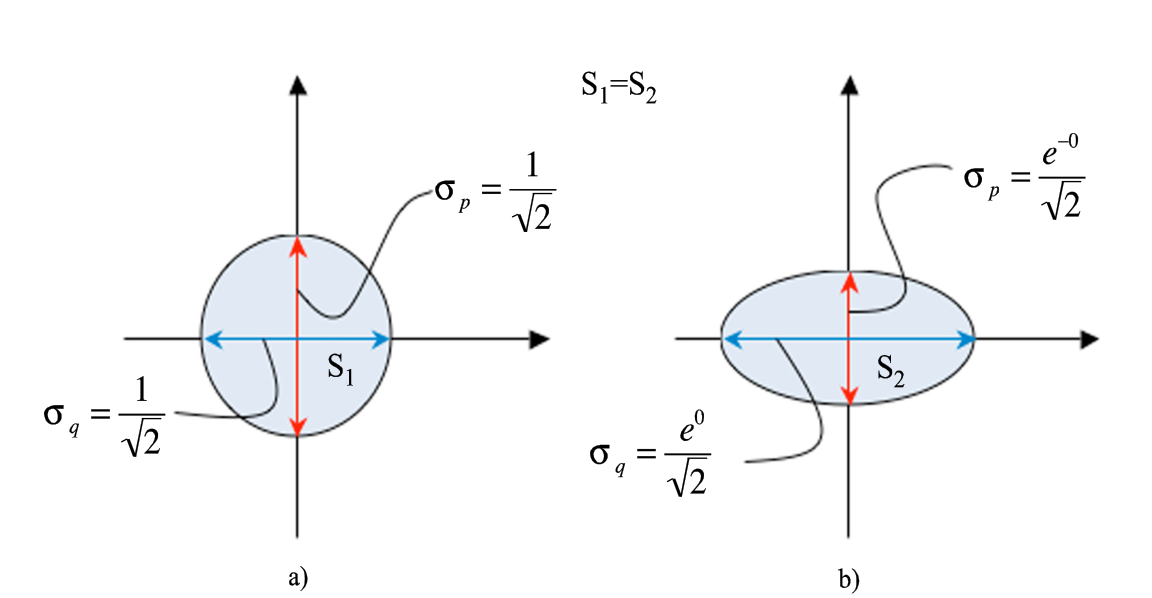
\includegraphics[max width=0.85\linewidth,keepaspectratio]{fig7_1.png}
\caption{产生--湮灭算子代数：能级图。}
\label{fig:7.1}
\end{figure}

% ch8.tex — 练习与补充 IV（中文版）
\chapter{练习与补充 IV}

\section{Sturm--Liouville 问题}

一般的 Sturm--Liouville 本征值问题是
\begin{equation}
-\frac{d}{dx}\!\left(p(x)\frac{dy}{dx}\right) + q(x)\,y = \lambda\,w(x)\,y,
\qquad x\in[a,b],
\label{eq:8.1.1}
\end{equation}
带自伴边界条件
$\alpha_1 y(a)+\alpha_2 y'(a)=0$，
$\beta_1 y(b)+\beta_2 y'(b)=0$。

本征值 $\lambda_n$ 是实数且有序排列
$\lambda_0<\lambda_1<\lambda_2<\cdots$，本征函数正交：
\begin{equation}
\int_a^b y_n(x)\,w(x)\,y_m(x)\,dx = N_n\delta_{nm}.
\label{eq:8.1.2}
\end{equation}

完备性：任何满足边界条件的 $f(x)$ 都可以展开为
$f(x)=\sum_n c_n y_n(x)$，其中
$c_n = \frac{1}{N_n}\int_a^b f(x)w(x)y_n(x)dx$。

\begin{exercise}
对 $[0,\pi]$ 上 $p=1$、$q=0$、$w=1$、带 Dirichlet 边界条件的情形，
求 $\lambda_n$、$y_n(x)$ 并验证正交性。
\end{exercise}

\section{Green 函数}

对于 $\hat L y = s(x)$，解为
\begin{equation}
y(x) = \int_a^b G(x,\xi)\,s(\xi)\,d\xi,
\label{eq:8.2.1}
\end{equation}
其中 Green 函数满足
$(\hat L-\lambda)G(x,\xi) = \delta(x-\xi)$（或 $\lambda=0$ 时 $\hat L G=\delta$）。

按本征函数展开构造：
\begin{equation}
G(x,\xi) = \sum_{n=0}^{\infty}\frac{y_n(x)\,y_n(\xi)}{N_n(\lambda_n-\lambda)}.
\label{eq:8.2.2}
\end{equation}

二阶 ODE 的跳跃条件：
$\left.\frac{\partial G}{\partial x}\right|_{x=\xi^+}
-\left.\frac{\partial G}{\partial x}\right|_{x=\xi^-} = \frac{1}{p(\xi)}$。

\begin{exercise}
对 $[0,1]$ 上 $y''=s(x)$ 且 $y(0)=y(1)=0$ 构造 $G(x,\xi)$，
并验证 $\int_0^1 G(x,\xi)\,d\xi = x(1-x)/2$。
\end{exercise}

\section{Laguerre 多项式、相关算子与 PDE}

Laguerre 导数是
$\hat\Lambda = x\frac{d^2}{dx^2}+(1-x)\frac{d}{dx}$。
它作用于 Laguerre 多项式为
\begin{equation}
\hat\Lambda L_n(x) = -n\,L_n(x).
\label{eq:8.3.1}
\end{equation}

Laguerre 热方程
$\partial_t F = \hat\Lambda F$（$F(x,0)=x^n$）
的解为
\begin{equation}
F(x,t) = L_n\!\left(\frac{x}{1-t}\right)(1-t)^n,
\qquad |t|<1.
\label{eq:8.3.2}
\end{equation}

Umbral 表示：
$L_n(x)=(\hat\theta)_n\,e^{-x\hat\theta}$，其中
$(\hat\theta)_n=\hat\theta(\hat\theta-1)\cdots(\hat\theta-n+1)$
且 $\hat\theta e^{-x\hat\theta}=e^{-x\hat\theta}$。

\begin{exercise}
用 umbral 表示验证 \eqref{eq:8.3.1}，并推导生成函数
$\sum_{n=0}^\infty L_n(x)t^n = e^{-xt/(1-t)}/(1-t)$。
\end{exercise}

\section{Appell 多项式、相关算子与偏微分方程}

Appell 多项式 $A_n(x)$ 满足
$\frac{d}{dx}A_n(x)=n\,A_{n-1}(x)$，并由
\begin{equation}
\sum_{n=0}^{\infty} A_n(x)\,\frac{t^n}{n!}=e^{x t}\,A(t),
\qquad A(0)=1.
\label{eq:8.4.1}
\end{equation}
生成。

满足 $\hat D_A A_n(x)=n\,A_{n-1}(x)$ 的相关求导算子 $\hat D_A$ 通过
$F(x,t)=e^{t\hat D_A}P(x)$ 求解 Cauchy 问题
$\partial_t F=\hat D_A F$，$F(x,0)=P(x)$。

\begin{exercise}
对于 $A_n(x)=x^n$（普通单项式），证明
$\hat D_A=\frac{d}{dx}$，并从 $e^{t\hat D_A}$ 恢复 Taylor 定理。
\end{exercise}

\section{Riemann 函数}

Riemann 方法求解二阶双曲型 PDE 的 Cauchy 问题。对于
\begin{equation}
\frac{\partial^2 u}{\partial x\partial y} + a(x,y)\frac{\partial u}{\partial x}
+ b(x,y)\frac{\partial u}{\partial y} + c(x,y)u = 0,
\label{eq:8.5.1}
\end{equation}
Riemann--Green 函数 $R(x,y;\xi,\eta)$ 满足带特征边界条件的伴随方程。

带非特征曲线上的 Cauchy 数据的解为
\begin{equation}
u(P) = \frac12\left[u(A)R(P;A)+u(B)R(P;B)\right]
+ \frac12\int_{AB}\left(R\frac{\partial u}{\partial n}-u\frac{\partial R}{\partial n}\right)ds.
\label{eq:8.5.2}
\end{equation}

\begin{exercise}
对于一维波动方程 $u_{xy}=0$，证明 $R=1$ 并恢复 d'Alembert 公式。
\end{exercise}

\section{Bessel 特殊函数}

Bessel 函数 $J_n(x)$ 满足
\begin{equation}
x^2J_n''+xJ_n'+(x^2-n^2)J_n=0,
\label{eq:8.6.1}
\end{equation}
生成函数为
\begin{equation}
e^{\frac{x}{2}(t-1/t)} = \sum_{n=-\infty}^{\infty} J_n(x)\,t^n.
\label{eq:8.6.2}
\end{equation}

递推关系：
\begin{align}
J_{n-1}+J_{n+1} &= \frac{2n}{x}J_n,\\
J_{n-1}-J_{n+1} &= 2J_n'.
\label{eq:8.6.3}
\end{align}

有限区间上带权重 $x$ 的正交性：
\begin{equation}
\int_0^a x\,J_n\!\left(\frac{\alpha_{nm}}{a}x\right)
J_n\!\left(\frac{\alpha_{nk}}{a}x\right)dx
= \frac{a^2}{2}J_{n+1}^2(\alpha_{nm})\,\delta_{mk},
\label{eq:8.6.4}
\end{equation}
其中 $\alpha_{nm}$ 是 $J_n$ 的第 $m$ 个零点。

修正 Bessel 函数：$I_n(x)=i^{-n}J_n(ix)$ 满足
$x^2I_n''+xI_n'-(x^2+n^2)I_n=0$。

Hankel 函数：$H_n^{(1)}=J_n+iY_n$，
$H_n^{(2)}=J_n-iY_n$，描述出射/入射柱波。

\begin{exercise}
由生成函数 \eqref{eq:8.6.2} 推导递推关系 \eqref{eq:8.6.3}。
\end{exercise}

\begin{exercise}
利用 $J_0$ 的 Laplace 变换计算 $\int_0^\infty e^{-ax}J_0(bx)\,dx=1/\sqrt{a^2+b^2}$。
\end{exercise}

% 图形
\begin{figure}[h]
\centering
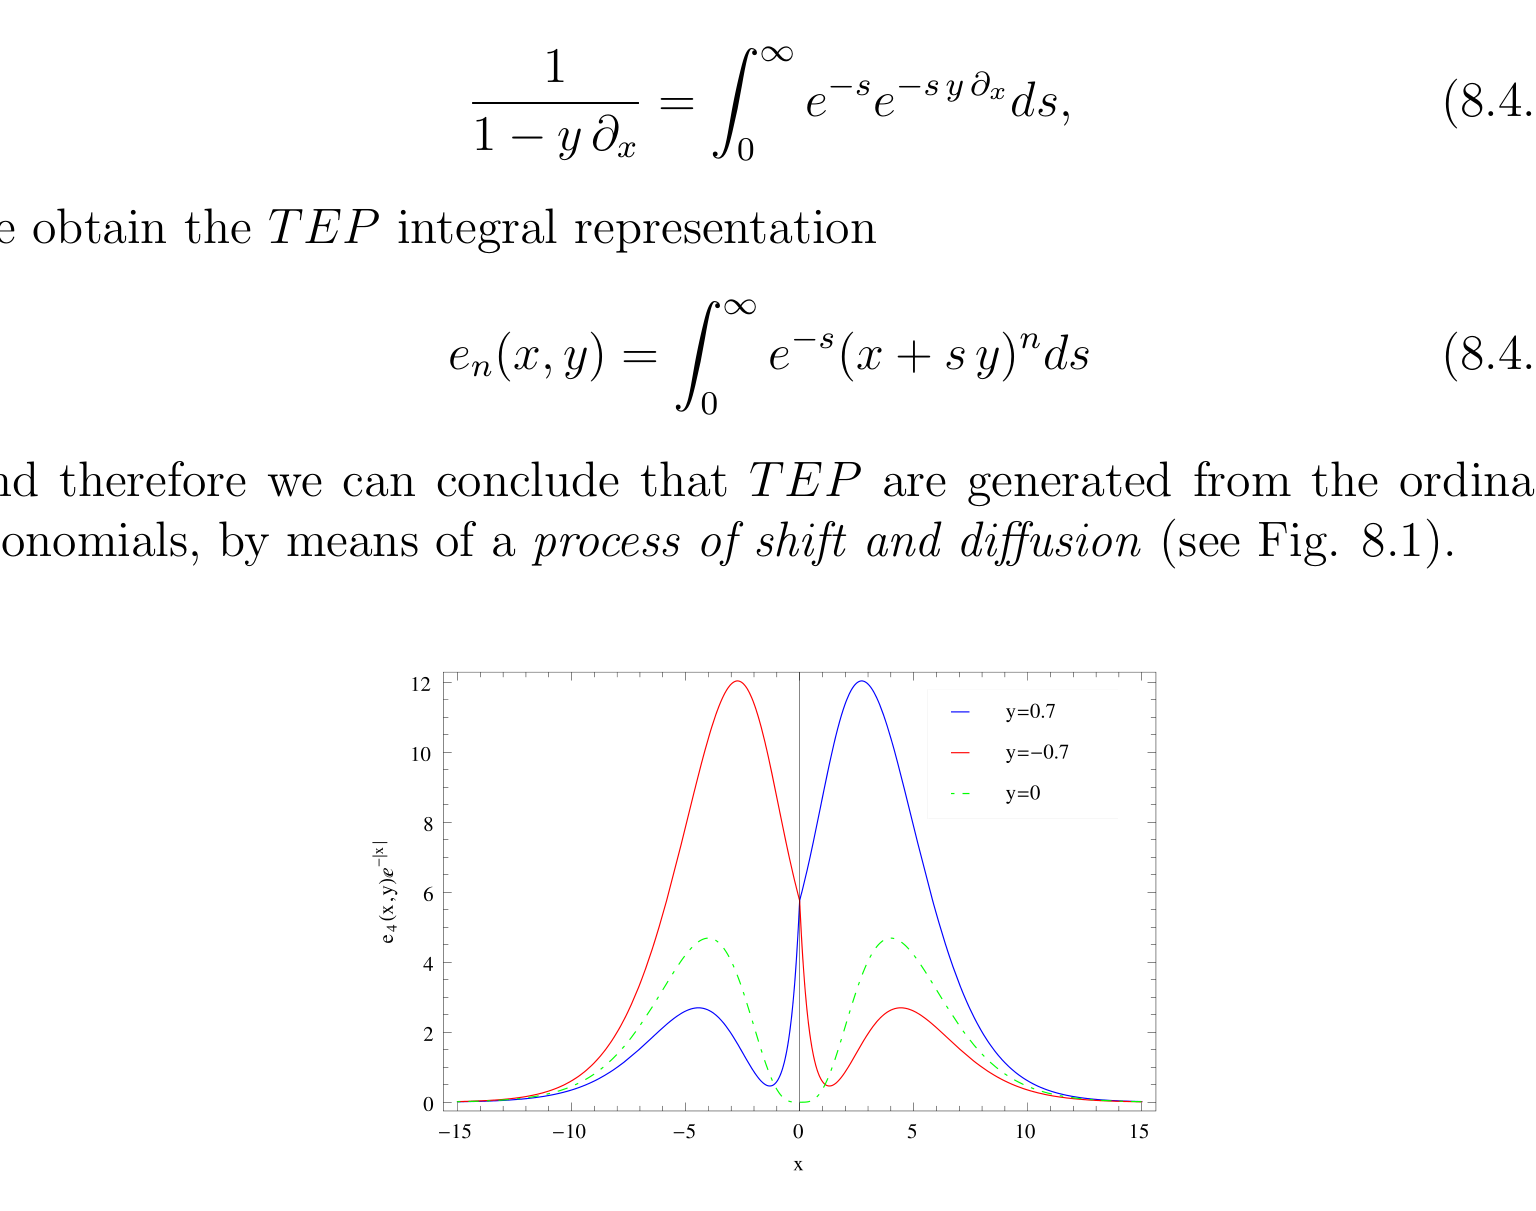
\includegraphics[max width=0.85\linewidth,keepaspectratio]{fig8_1.png}
\caption{Bessel 函数 $J_n(x)$，$n=0,1,2,3$。}
\label{fig:8.1}
\end{figure}

\begin{figure}[h]
\centering
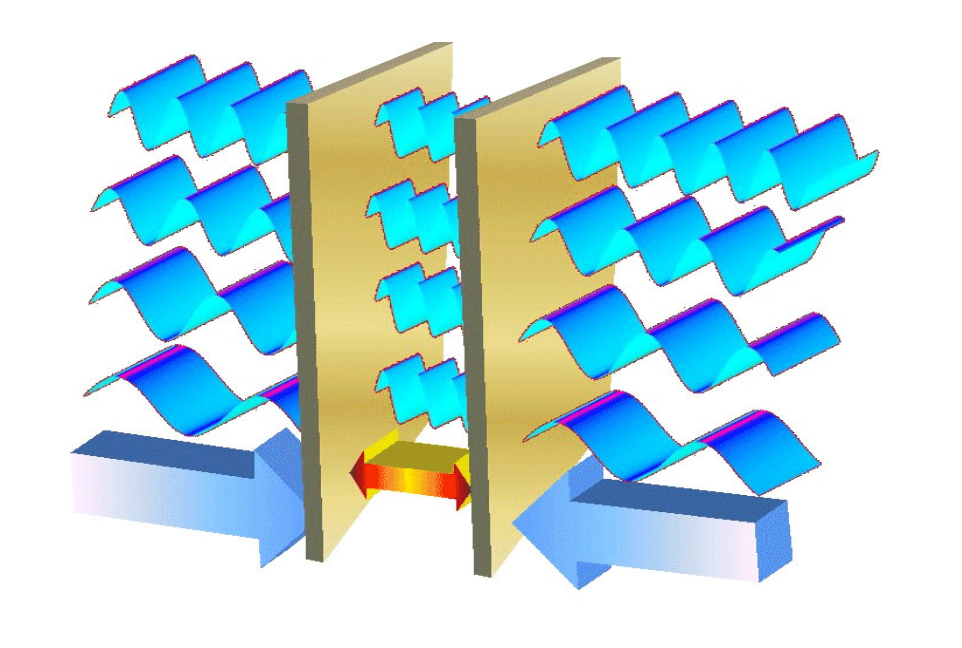
\includegraphics[max width=0.85\linewidth,keepaspectratio]{fig8_3.png}
\caption{波动方程的 Riemann 函数。}
\label{fig:8.3}
\end{figure}

% ch9.tex — 特殊函数、Umbral 方法及其应用（中文版）
\chapter{特殊函数、Umbral 方法及其应用}

\section{Umbral 方法导论及相应应用}

Umbral 演算把满足 $\hat\theta x^n = x\,x^{n-1}$ 的指标移位算子 $\hat\theta$ 形式上当作一个数来处理。它把特殊多项式的恒等式转化为代数运算。

对于任何 $\deg P_n=n$ 的多项式族 $P_n(x)$，引入 umbral 算子 $\hat\theta$，使得
\begin{equation}
\hat\theta^n\cdot 1 = P_n(x),
\label{eq:9.1.1}
\end{equation}
其中点表示作用于``真空'' $1$。

加法公式：若 $P_n(x+y)=\sum_k\binom{n}{k}P_k(x)P_{n-k}(y)$，在 umbral 记号下它变为
$(\hat\theta_1+\hat\theta_2)^n\cdot1 = \sum_k\binom{n}{k}\hat\theta_1^k\hat\theta_2^{n-k}\cdot1$。

\begin{exercise}
通过把 $\hat\theta$ 等同于乘以 $x$，证明 umbral 方法重现 $(x+y)^n$ 的二项式定理。
\end{exercise}

\section{关于 Umbral 方法、无穷积分与 Borel 变换的进一步说明}

形式级数
$f(z)=\sum_{n=0}^\infty a_n z^n$ 的 Borel 变换为
\begin{equation}
\mathcal B[f](s) = \sum_{n=0}^\infty \frac{a_n}{n!}\,s^n.
\label{eq:9.2.1}
\end{equation}

若 $\mathcal B[f](s)$ 的收敛半径非零，原级数可以通过逆 Borel 变换
\begin{equation}
f(z) = \int_0^\infty e^{-t}\,\mathcal B[f](zt)\,dt,
\label{eq:9.2.2}
\end{equation}
恢复，前提是该积分收敛。

Borel 变换把阶乘型发散微扰级数转化为收敛级数，是渐近展开重整求和的基石。

\begin{exercise}
计算 $\sum_{n=0}^\infty n!\,z^n$ 的 Borel 变换，并证明逆 Borel 积分重现原渐近级数。
\end{exercise}

\section{Borel 变换及其应用}

\subsection{Borel--Pad\'e}

Borel 变换的 Pad\'e 近似加速收敛，并从微扰级数中提取非微扰信息。

给定 Borel 变换 $B(s)=\sum b_n s^n$，构造 $[N/M]$ 阶 Pad\'e 近似 $B_{[N/M]}(s)=P_N(s)/Q_M(s)$，然后
\begin{equation}
f_{\rm BP}(z) = \int_0^\infty e^{-t}\,B_{[N/M]}(zt)\,dt.
\label{eq:9.3.1}
\end{equation}

这种 Borel--Pad\'e 方法被广泛用于量子场论与统计力学中对发散微扰级数求和。

\begin{exercise}
对于 $B(s)=1/(1-s)$，计算 $[1/1]$ 阶 Pad\'e 近似并计算 Borel--Pad\'e 积分。
\end{exercise}

\section{Umbral 形式体系与 Laguerre 多项式}

Laguerre 多项式可以用 umbral 表示为
\begin{equation}
L_n(x) = (\hat\theta)_n\,e^{-x\hat\theta},
\qquad (\hat\theta)_n = \hat\theta(\hat\theta-1)\cdots(\hat\theta-n+1),
\label{eq:9.4.1}
\end{equation}
使递推关系代数化。

生成函数变为
\begin{equation}
\sum_{n=0}^\infty L_n(x)\,t^n
= \frac{1}{1-t}\,\exp\!\left(-\frac{xt}{1-t}\right),
\label{eq:9.4.2}
\end{equation}
它由 umbral 移位得出，注意到
$e^{-x\hat\theta}\cdot(1-t)^{-\hat\theta}=e^{-x\hat\theta/(1-t)}$。

正交性：
\begin{equation}
\int_0^\infty e^{-x}L_n(x)L_m(x)\,dx = \delta_{nm}.
\label{eq:9.4.3}
\end{equation}

\begin{exercise}
用 umbral 表示证明三项递推
$(n+1)L_{n+1}(x)=(2n+1-x)L_n(x)-nL_{n-1}(x)$。
\end{exercise}

\section{Umbral 形式体系与 Hermite 多项式}

Hermite 多项式的 umbral 形式：
\begin{equation}
H_n(x) = (\hat\theta+x)^n\cdot 1,
\qquad \hat\theta\frac{d}{dx}=1.
\label{eq:9.5.1}
\end{equation}

生成函数：
\begin{equation}
\sum_{n=0}^\infty H_n(x)\,\frac{t^n}{n!}
= \exp(2xt-t^2),
\label{eq:9.5.2}
\end{equation}
由 $e^{t(\hat\theta+x)}\cdot1=e^{xt}e^{-t^2}$ 得出，其中用到 $\hat\theta\cdot1=0$、$\hat\theta x^n=nx^{n-1}$。

正交性：
\begin{equation}
\int_{-\infty}^{\infty} e^{-x^2}H_n(x)H_m(x)\,dx
= 2^n n!\sqrt{\pi}\,\delta_{nm}.
\label{eq:9.5.3}
\end{equation}

\begin{exercise}
从 umbral 表示推导递推 $H_{n+1}(x)=2xH_n(x)-2nH_{n-1}(x)$。
\end{exercise}

\section{Umbral 形式体系与算子排序}

Wei--Norman 与 Weyl 排序得以简化：umbral 移位把对易子化为 c 数系数。

对于 $[\hat A,\hat B]=k\hat 1$，Weyl 恒等式
$e^{\hat A+\hat B}=e^{\hat A}e^{\hat B}e^{-k/2}$
通过注意到在 umbral 形式下对易子变为简单的移位而得到。

Umbral 记号下的 Crofton 恒等式：
\begin{equation}
e^{\xi\hat A}\hat B^n = (\hat B+\xi k)^n e^{\xi\hat A},
\label{eq:9.6.1}
\end{equation}
它由 $\hat A\hat B^n - \hat B^n\hat A = nk\hat B^{n-1}$ 得出。

\begin{exercise}
用 umbral 方法推导二阶 BCH 公式：
$e^{\hat A}e^{\hat B}=e^{\hat A+\hat B+\frac12[\hat A,\hat B]}$。
\end{exercise}

\section{Mittag-Leffler 函数与分数阶微积分应用}

Mittag-Leffler 函数推广了指数函数：
\begin{equation}
E_\alpha(z) = \sum_{n=0}^{\infty}\frac{z^n}{\Gamma(\alpha n+1)},
\qquad \alpha>0.
\label{eq:9.7.1}
\end{equation}

特殊情况：$E_1(z)=e^z$，$E_2(z^2)=\cosh z$，
$E_{1/2}(-\sqrt{z})=e^{-z}\erfc(\sqrt{z})$。

分数阶微分方程：
\begin{equation}
\frac{d^\alpha}{dt^\alpha}F(t) = \lambda F(t), \qquad F(0)=1,
\label{eq:9.7.2}
\end{equation}
的解为 $F(t)=E_\alpha(\lambda t^\alpha)$。

分数阶扩散：$\partial_t^\alpha F = D\,\partial_x^2 F$ 的基本解用 $E_\alpha$ 与热核表示。

\begin{exercise}
证明 $\alpha=1/2$ 时的 $E_\alpha(z)$ 化为误差函数，并求解 $\alpha=1/2$ 的分数阶弛豫方程。
\end{exercise}

\section{负导数形式体系与定积分}

作用于多项式的负导数 $\partial_x^{-1}$ 产生积分：$\partial_x^{-1}x^n = x^{n+1}/(n+1)$。

迭代给出 Riemann--Liouville 分数阶积分：
\begin{equation}
\partial_x^{-\nu}f(x) = \frac{1}{\Gamma(\nu)}\int_0^x (x-t)^{\nu-1}f(t)\,dt,
\qquad \nu>0.
\label{eq:9.8.1}
\end{equation}

分数阶导数由 $\partial_x^\alpha = \partial_x^n\circ\partial_x^{\alpha-n}$ 定义，
其中 $n-1<\alpha<n$。

在 umbral 语言中，$\partial_x^{-\nu}$ 对应于适当基中的移位算子
$\hat\theta\mapsto\hat\theta+\nu$。

\begin{exercise}
用 Riemann--Liouville 定义计算 $\partial_x^{-1/2}1$ 与 $\partial_x^{-1/2}x$。
\end{exercise}

\section{Umbral 形式体系、对偶数与超 Gauss 光束传输}

对偶数 $(a+b\epsilon,\epsilon^2=0)$ 与 umbral 移位结合，可以模拟超 Gauss 激光束及其 ABCD 传输。

对偶数 $\hat z_\pm = x\hat 1\pm\epsilon y$ 作用于函数为
\begin{equation}
f(\hat z_\pm) = f(x)\hat 1 \pm \epsilon y\,f'(x).
\label{eq:9.9.1}
\end{equation}

矩阵实现：
\begin{equation}
f(\hat z_+) = \mat{f(x)&yf'(x)\\0&f(x)},\qquad
f(\hat z_-) = \mat{f(x)&0\\yf'(x)&f(x)}.
\label{eq:9.9.2}
\end{equation}

超 Gauss 光束：强度分布 $I(r)=I_0\exp[-(r/w)^n]$，其中
$n>2$（平顶）。光束穿过光学元件的传输由推广到对偶数相空间的 ABCD 定律描述。

\begin{exercise}
证明对偶数代数蕴含
$f(\hat z_+)g(\hat z_+) = (fg)(\hat z_+)$（函数复合）。
\end{exercise}

\begin{exercise}
用对偶数形式体系推导超 Gauss 光束穿过焦距为 $f$ 的透镜的传输矩阵。
\end{exercise}

% 图形
\begin{figure}[h]
\centering
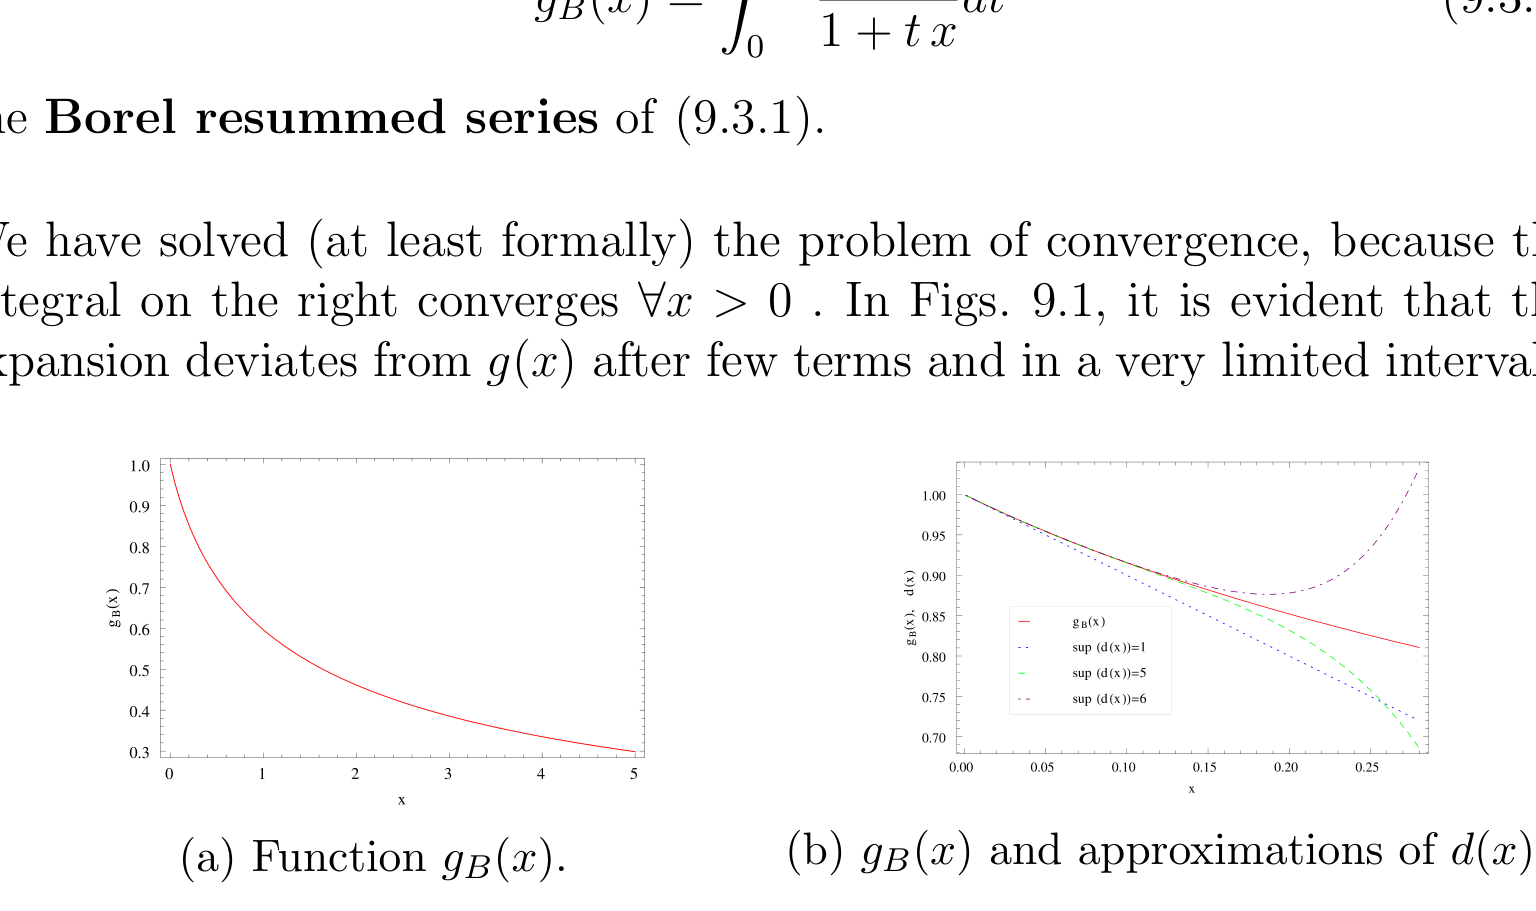
\includegraphics[max width=0.85\linewidth,keepaspectratio]{fig9_1.png}
\caption{不同 $\alpha$ 的 Mittag-Leffler 函数 $E_\alpha(z)$。}
\label{fig:9.1}
\end{figure}

\begin{figure}[h]
\centering
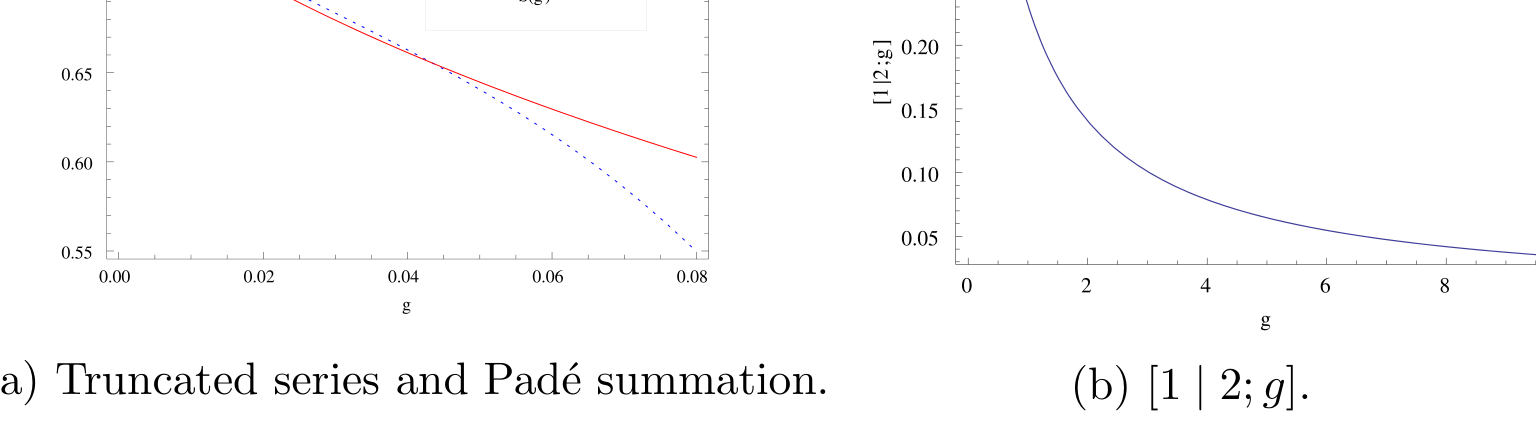
\includegraphics[max width=0.85\linewidth,keepaspectratio]{fig9_4.png}
\caption{分数阶扩散：不同时刻的解剖面。}
\label{fig:9.4}
\end{figure}

\begin{figure}[h]
\centering
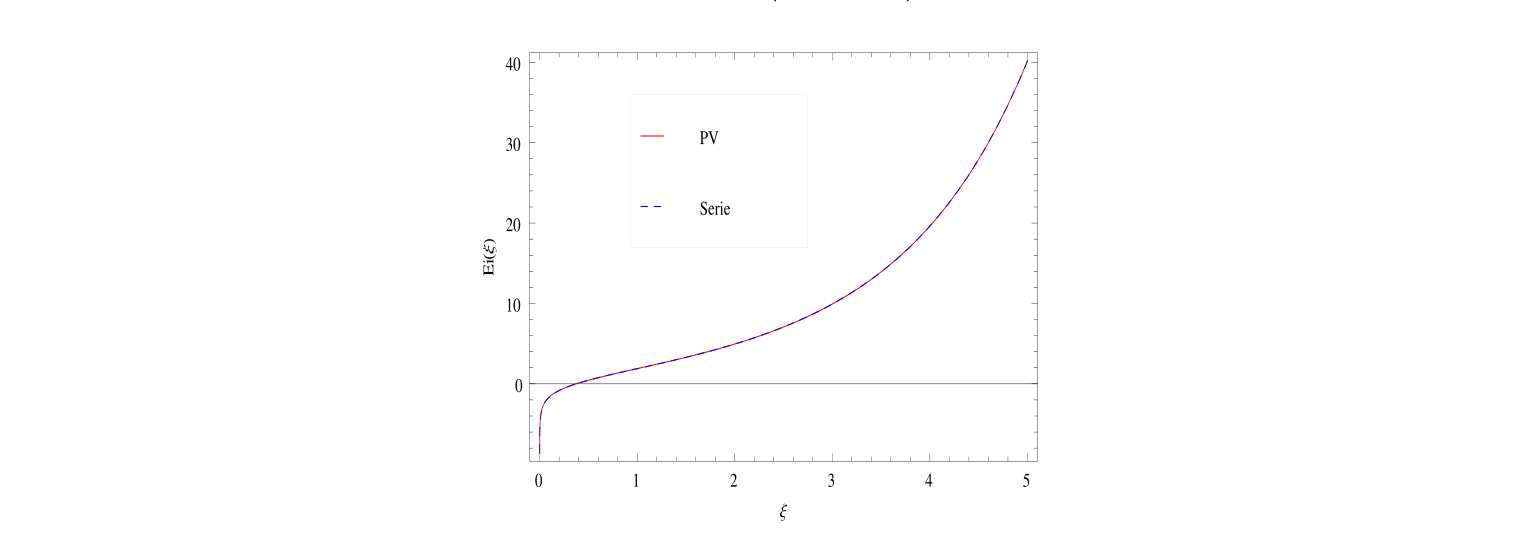
\includegraphics[max width=0.85\linewidth,keepaspectratio]{fig9_9.png}
\caption{超 Gauss 光束穿过光学系统的传输。}
\label{fig:9.9}
\end{figure}

% ch10.tex — 初窥 Feynman 图的数学（中文版）
\chapter{初窥 Feynman 图的数学}

\section{引言：非相对论散射理论与 Lippmann--Schwinger 方程}

Lippmann--Schwinger 方程是散射态定态 Schr\"odinger 方程的积分形式：
\begin{equation}
|\psi^{(\pm)}\rangle = |k\rangle
+ \frac{1}{E-H_0\pm i0}\,\hat V\,|\psi^{(\pm)}\rangle,
\label{eq:10.1.1}
\end{equation}
其中 $|k\rangle$ 是动量为 $\hbar k$、能量为 $E=\hbar^2k^2/(2m)$ 的自由粒子态。

自由哈密顿量的 Green 函数为
\begin{equation}
G_0^{(\pm)}(E) = \frac{1}{E-H_0\pm i0}
= \lim_{\epsilon\to0^+}\frac{1}{E-H_0\pm i\epsilon}.
\label{eq:10.1.2}
\end{equation}

$S$ 矩阵联系入射与出射渐近态：
$S_{fi}=\delta_{fi}-2\pi i\,\delta(E_f-E_i)\,T_{fi}$，其中
$T_{fi}=\langle f|\hat V|\psi_i^{(+)}\rangle$。

\begin{exercise}
通过对 $E-H_0\pm i0$ 求逆，从 $(E-H_0)\psi=V\psi$ 推导 Lippmann--Schwinger 方程。
\end{exercise}

\section{Fermi 黄金规则}

从初态 $|i\rangle$ 到连续谱 $\{|f\rangle\}$ 的跃迁率由 Fermi 黄金规则给出：
\begin{equation}
\Gamma_{i\to f} = \frac{2\pi}{\hbar}\,
\bigl|\langle f|\hat V|i\rangle\bigr|^2\,\rho(E_f),
\label{eq:10.2.1}
\end{equation}
其中 $\rho(E_f)$ 是末态密度。

\subsection{Fermi 黄金规则的应用}

对于通过发射能量为 $\hbar\omega=E_e-E_g$ 的光子从激发态 $|e\rangle$ 衰变到基态 $|g\rangle$ 的原子，
\begin{equation}
\Gamma_{e\to g} = \frac{4\alpha\omega^3}{3c^2}\,
\bigl|\langle g|\vect r|e\rangle\bigr|^2,
\label{eq:10.2.2}
\end{equation}
其中 $\alpha=e^2/(4\pi\epsilon_0\hbar c)$ 是精细结构常数。

\begin{exercise}
从最小耦合哈密顿量
$\hat H_{\rm int}=-(e/m)\vect A\cdot\vect p$ 与 Fermi 黄金规则推导 \eqref{eq:10.2.2}。
\end{exercise}

\section{Feynman 图：入门规则}

对于标量 $\phi^4$ 理论，$\mathcal L_{\rm int}=-\frac{\lambda}{4!}\phi^4$，
Feynman 规则为：
\begin{itemize}
\item 传播子：每条内线对应 $\tilde\Delta_F(k)=\frac{1}{k^2-m^2+i0}$。
\item 顶点：每个四顶点给出因子 $-i\lambda$。
\item 动量守恒：每个顶点处 $\delta^{(4)}(\sum p_{\rm in}-\sum p_{\rm out})$。
\item 对称因子：每个图给出 $1/S$。
\end{itemize}

对于 QED，顶点为 $-ie\gamma^\mu$，光子传播子为
$-ig_{\mu\nu}/(k^2+i0)$。

\begin{exercise}
画出 $\phi^4$ 理论中 $2\to2$ 散射的两个树级 Feynman 图，并写出相应的振幅。
\end{exercise}

\section{虚粒子与传播子}

离壳内线携带不满足 $k^2=m^2$ 的动量 $k$。
传播子通过 $i0$ 处方编码因果性：
\begin{equation}
\Delta_F(x-y) = \int\frac{d^4k}{(2\pi)^4}\,
\frac{e^{-ik\cdot(x-y)}}{k^2-m^2+i0}.
\label{eq:10.4.1}
\end{equation}

$i0$ 处方选择 Feynman 围道：正能量的粒子随时间向前传播，负能量的反粒子向后传播。

\begin{exercise}
证明 Feynman 传播子满足
$(\Box+m^2)\Delta_F(x-y)=-\delta^{(4)}(x-y)$。
\end{exercise}

\section{类空与类时 Feynman 图}

$q^2=(p_1-p_2)^2$ 的符号区分
类空（$q^2<0$）与类时（$q^2>0$）动量转移，
两者的传播子解析结构不同。

对于类空 $q^2<0$，传播子 $\sim 1/|q^2|$ 是实的（没有在壳中间态）。对于类时 $q^2>0$，传播子通过 $i0$ 发展出虚部（可能产生在壳态）。

\begin{exercise}
对于 $e^+e^-\to\mu^+\mu^-$，判断交换的虚光子是类空还是类时，并计算 $q^2$。
\end{exercise}

\section{Dirac Gamma 矩阵}

Clifford 代数：
\begin{equation}
\{\gamma^\mu,\gamma^\nu\} = 2\eta^{\mu\nu}\hat 1,
\qquad \eta={\rm diag}(-1,1,1,1).
\label{eq:10.6.1}
\end{equation}

显式 Dirac 表示（$2\times2$ 分块）：
\begin{align}
\gamma^0 &= \mat{\hat 1&\hat 0\\\hat 0&-\hat 1},\\
\gamma^i &= \mat{\hat 0&\hat\sigma_i\\-\hat\sigma_i&\hat 0},\\
\gamma^5 &= i\gamma^0\gamma^1\gamma^2\gamma^3
= \mat{\hat 0&\hat 1\\\hat 1&\hat 0}.
\label{eq:10.6.2}
\end{align}

关键恒等式：
\begin{align}
\gamma^\mu\gamma^\nu+\gamma^\nu\gamma^\mu &= 2\eta^{\mu\nu},\\
\tr(\gamma^\mu\gamma^\nu) &= 4\eta^{\mu\nu},\\
\tr(\gamma^5\gamma^\mu\gamma^\nu) &= 0,\\
\gamma^5\gamma^\mu+\gamma^\mu\gamma^5 &= 0.
\label{eq:10.6.3}
\end{align}

手征投影算子：$P_L=\frac12(1-\gamma^5)$，$P_R=\frac12(1+\gamma^5)$。

\begin{exercise}
验证 Dirac 表示满足 Clifford 代数，且 $(\gamma^5)^2=\hat 1$。
\end{exercise}

\section{Dirac 方程的数学}

自由粒子的 Dirac 方程：
\begin{equation}
(i\gamma^\mu\partial_\mu - m)\psi(x) = 0.
\label{eq:10.7.1}
\end{equation}

平方后给出 Klein--Gordon 方程：
$(-\Box-m^2)\psi=0$，证实了正确的相对论色散关系。

平面波解：
\begin{equation}
u(p,s) = \sqrt{\frac{E+m}{2m}}
\mat{\chi_s\\\frac{\vect\sigma\cdot\vect p}{E+m}\chi_s},\qquad
v(p,s) = \sqrt{\frac{E+m}{2m}}
\mat{\frac{\vect\sigma\cdot\vect p}{E+m}\chi_s\\\chi_s},
\label{eq:10.7.2}
\end{equation}
分别对应粒子（$u$）与反粒子（$v$），旋量 $\chi_s$。

Dirac 伴随为 $\bar\psi=\psi^\dagger\gamma^0$，守恒流为 $j^\mu=\bar\psi\gamma^\mu\psi$。

\begin{exercise}
证明 $u^\dagger(p,s)u(p,s')=2E\delta_{ss'}$ 且
$\bar u(p,s)u(p,s')=2m\delta_{ss'}$。
\end{exercise}

\section{略谈量子电动力学}

QED 顶点通过 $-ie\gamma^\mu$ 把电子与光子耦合起来。
第 7 章的 Dyson 级数生成微扰 $S$ 矩阵与 Feynman 图。

QED 拉格朗日量：
\begin{equation}
\mathcal L_{\rm QED} = \bar\psi(i\slashed\partial-m)\psi
- \frac14 F_{\mu\nu}F^{\mu\nu} - e\bar\psi\gamma^\mu\psi A_\mu,
\label{eq:10.8.1}
\end{equation}
其中 $\slashed\partial=\gamma^\mu\partial_\mu$，$F_{\mu\nu}=\partial_\mu A_\nu-\partial_\nu A_\mu$。

电子单圈自能给出质量重整化，真空极化修正光子传播子。

\begin{exercise}
写出动量空间中电子传播子的 Feynman 规则，并验证其在 $p^2=m^2$ 处的极点结构。
\end{exercise}

\section{物理中量纲与单位的形式观点}

量纲分析：每个物理量都有由 $[M]$、$[L]$、$[T]$、$[I]$ 等构建的量纲。

自然单位制：$\hbar=c=1$ 把所有量纲化为能量的幂次：
$[E]=[M]=[L]^{-1}=[T]^{-1}$。

Feynman 积分中的标度：圈积分
$\int d^4k/(2\pi)^4\,f(k,p)$ 的量纲为 $[E]^{4-n_f}$，其中 $n_f$
是分子中合并的质量量纲。

可重整化性：在 QED 中，自然单位制下耦合常数 $e$ 无量纲，使理论可重整化。

\begin{exercise}
在自然单位制下，证明精细结构常数
$\alpha=e^2/(4\pi)$ 无量纲，并计算其数值。
\end{exercise}

% 图形
\begin{figure}[h]
\centering
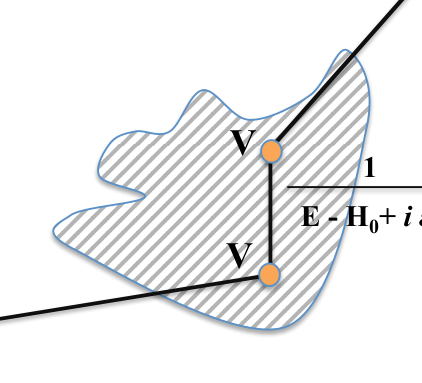
\includegraphics[max width=0.85\linewidth,keepaspectratio]{fig10_1.png}
\caption{Feynman 图：电子--正电子湮灭为两个光子。}
\label{fig:10.1}
\end{figure}

\begin{figure}[h]
\centering
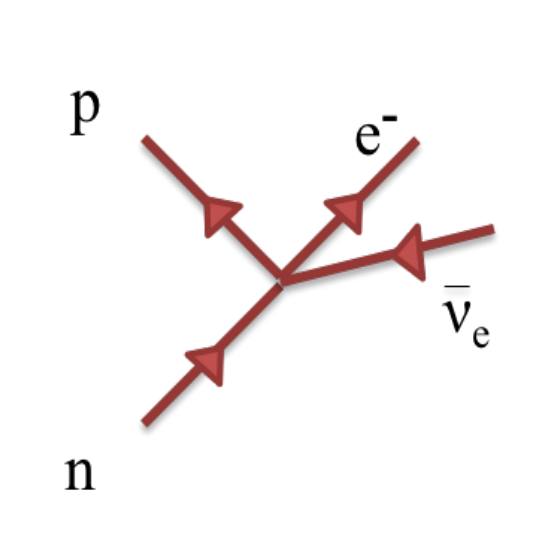
\includegraphics[max width=0.85\linewidth,keepaspectratio]{fig10_2.png}
\caption{$2\to2$ 散射的树级 Feynman 图。}
\label{fig:10.2}
\end{figure}

\begin{figure}[h]
\centering
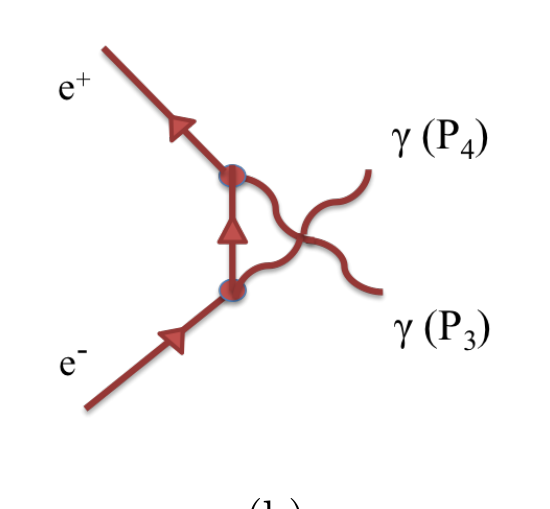
\includegraphics[max width=0.85\linewidth,keepaspectratio]{fig10_7.png}
\caption{电子传播子的单圈修正（自能）。}
\label{fig:10.7}
\end{figure}

\begin{figure}[h]
\centering
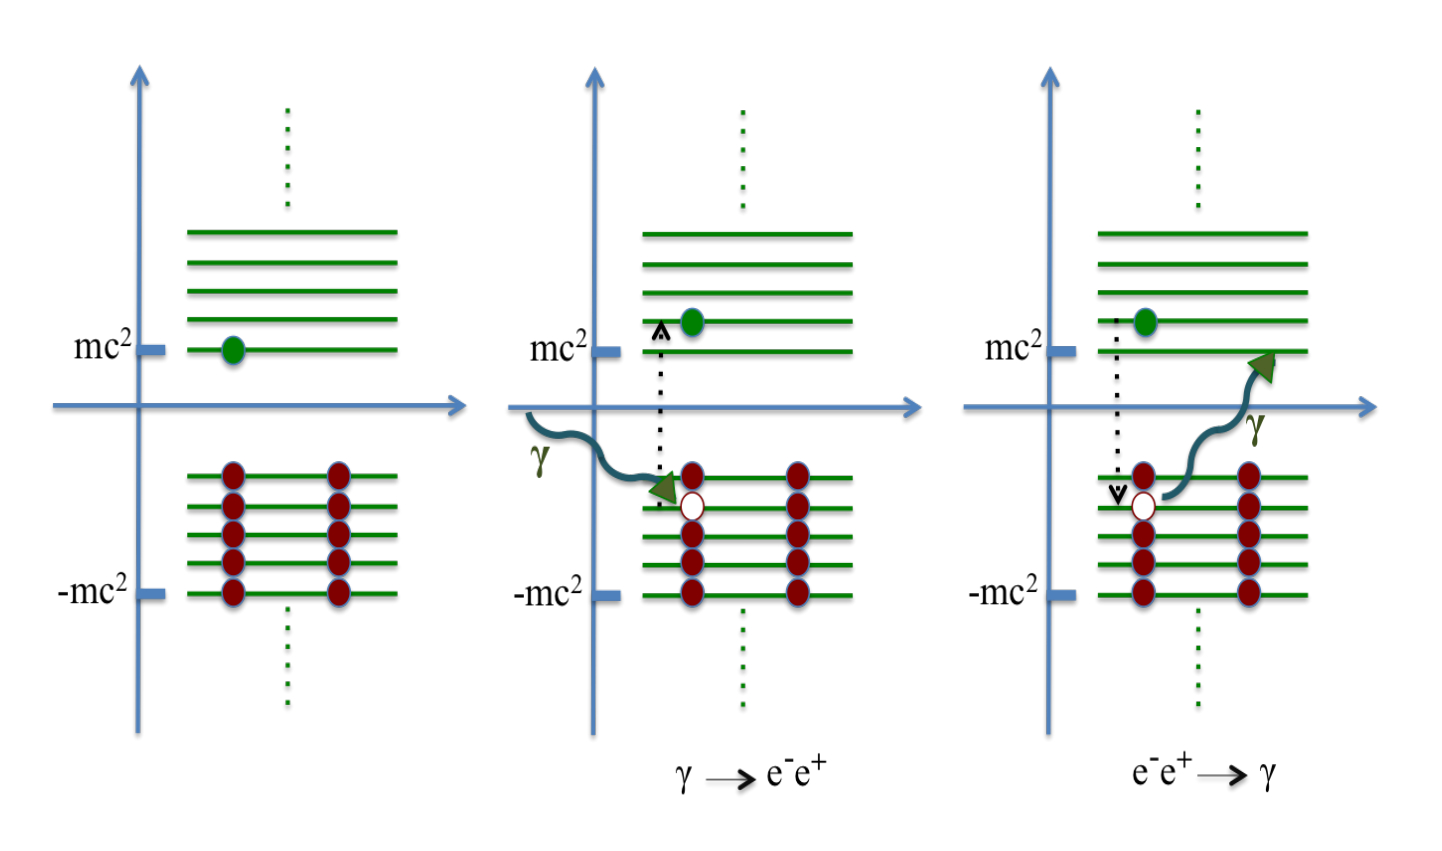
\includegraphics[max width=0.85\linewidth,keepaspectratio]{fig10_12.png}
\caption{真空极化：光子传播子的单圈修正。}
\label{fig:10.12}
\end{figure}

\begin{figure}[h]
\centering
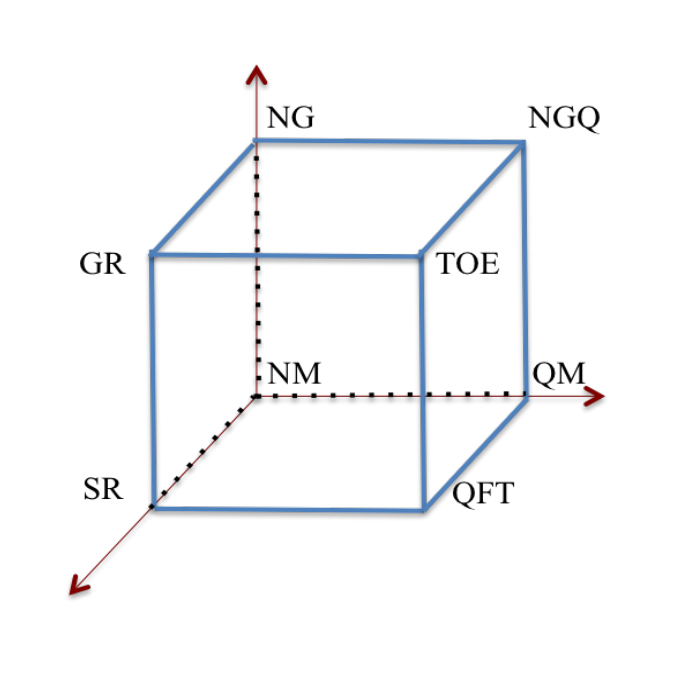
\includegraphics[max width=0.85\linewidth,keepaspectratio]{fig10_22.png}
\caption{Feynman 规则：顶点、传播子与对称因子约定。}
\label{fig:10.22}
\end{figure}


\end{document}
